\chapter{Adapting hardware to improve core composition performance}~\label{chp:hardchanges}

\section{Introduction}\label{sect:introduction-chapter3}
%replace the ref with actual latex ref
The previous chapter showed how reconfiguring a dynamic multicore processor at runtime can improve the efficiency of core composition as it is able to adapt to different phases of instructions per cycle (IPC).
It also demonstrated that there are certain limiting factors to how performant core composition can be.
The limiting factors discussed were branch prediction requirements and cost of synchronising cores.
To improve the performance of core composition, Chapters~\ref{chp:streamit} and ~\ref{chp:cases} showed that source level modifications are a good method.
These source-level modifications are often used to increase the size of the block which enables better utilisation of large core compositions.

Whilst source-level modifications do in fact improve the performance of large core compositions, they may not always be applicable.
In situations where source or compiler optimisations cannot increase the size of a block, core composition cannot improve the performance of the application.
To increase the viability of core composition, other solutions must therefore be explored.
Instead of solely focusing on improving the source code, analysing how a composition functions at a hardware level can help determine other potential bottlenecks in the system.

When modifications to software cannot yield any performance improvements, it is important to investigate if any hardware modifications can help increase the usefulness of core fusion.
By modifying how core composition behaves, this can potentially improve the performance on large compositions.
For example, modifying how blocks are distributed amongst cores can potentially increase the fairness of work distribution, increasing the efficiency of the composition.
This chapter explores the hardware bottlenecks that reduce the efficiency of core composition, and how to address these concerns.

There are two features of the processor that have a large impact on performance that are explored: first the block fetching mechanism in a composition, and data depenencies resolution between blocks can be handled.
The current fetching model focuses on filling the instruction window of a single core before activating another core in the composition.
Without modifications, this fetching model requires either large blocks to reduce the time required to activate multiple cores in a composition or a fast issue and dispatch width on the core, which increases the complexity of the design.
Thus, exploring how the fetching model can be modified to prioritise using all the cores in the composition over filling a single core can lead to better utilisation of the composition.

Secondly register dependencies can reduce block level paralellism which in turn makes core composition less useful.
Reduced block level parallelism due to data dependencies is similar to an issue found in superscalar processors~\cite{peraisBeBop2015}.
If register values could be predicted, instructions could fire speculatively which in turn would improve block level parallelism.
This chapter therefore explores how a value predictor, which predicts register values to reduce the data dependencies, can be used to improve performance in core composition.

This chapter is organised as follows: first a benchmark previously described in Chapter~\ref{chp:cases} is re-analysed to underline how current hardware does not suffice to ensure performance improvements.
Then a new fetching mechanism called Round Robin Fetch is introduced: cores are able to fetch blocks independently in a round robin fashion to improve fairness.
This is followed by a discussion of how value prediction can be used to resolve data dependencies between blocks and reduce performance penalties caused by the network on chip.
A current state-of-the art predictor is then discussed and shown to be applicable for the EDGE architecture.
Then an exploration of how these hardware modifications affect performance of core composition under an idealistic scenario, where perfect value prediction is enabled is conducted.
The benchmarks used in this chapter are the San-Diego Vision benchmark suite, the same as Chapter~\ref{chp:cases}.
Finally this is then followed by an evaluation of a real value predictor~\cite{peraisBeBop2015}, the block based differential VTAGE predictor (D-VTAGE).
Different parameters of the predictor are modified to understand how value prediction can be adapted to EDGE.

To summarise, the contributions are:

\vspace{-1em}
\begin{itemize}
\item A presentation of a new fetching scheme, Round Robin Fetch.
\vspace{-1em}
\item An analysis of how how value prediction can improve performance of core composition on the SD-VBS benchmark suite~\cite{sdvbs}.
\item An implementation and evaluation of the block-based VTAGE value predictor for EDGE, demonstrating that performance can be improved by only predicting register reads.
\end{itemize}
\section{Motivation}\label{sect:ch3-motivation}
This section explores how core composition performance depends on branch prediction, fetching mechanism, and data dependencies between blocks and how modifications to certain mechanisms can improve performance.
\vspace{-1em}
\subsection{Branch prediction}
\begin{figure}[t]
    \centering
    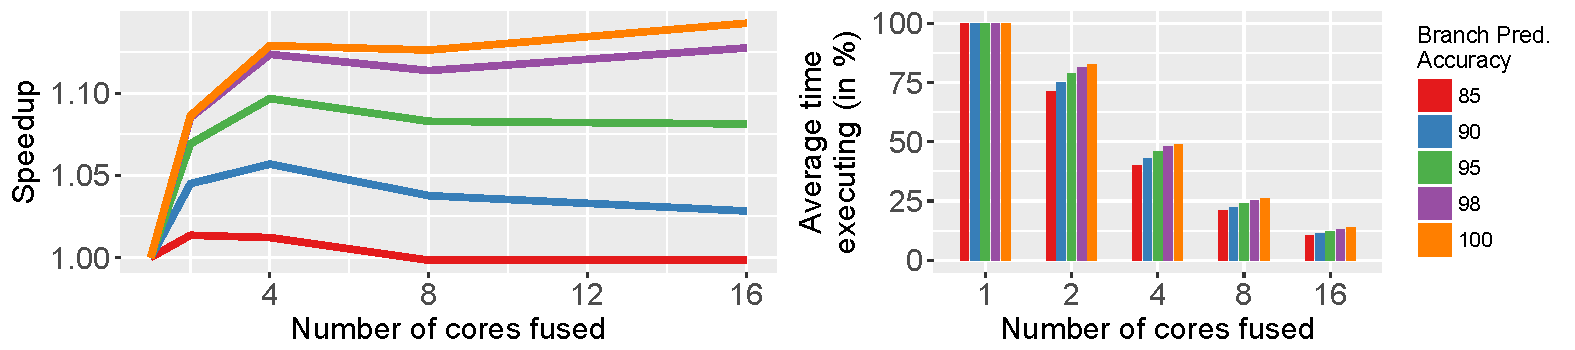
\includegraphics[width=1\textwidth]{chapter3/graphics/motiv_p1.pdf}
    \caption{Left: Speedup obtained when executing the MSER benchmark on different compositions and branch prediction accuracies.
	Right: Percentage of time (in cycles) cores in a composition execute instructions compared to the overall execution time. Higher is better for both.}
    \label{fig:mser_motiv}
    \centering
    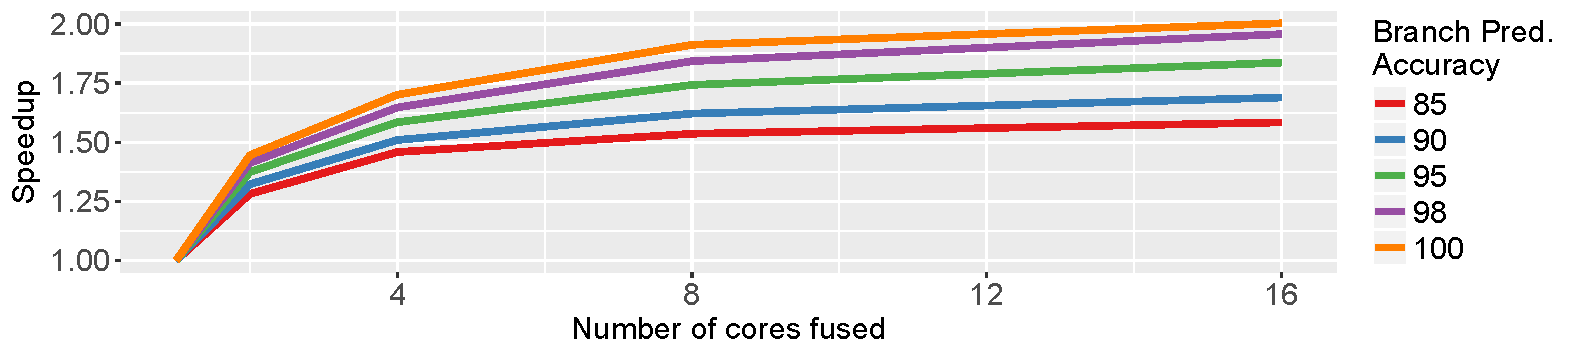
\includegraphics[width=1\textwidth]{chapter3/graphics/perfect_fetch_motiv2.pdf}
    \caption{Speedup obtained when executing the MSER benchmark with different core composition with an oracle fetching scheme and perfect branch prediction. Higher is better. }
    \label{fig:motivation_fetch}
	\vspace{1em}
\end{figure}
Chapter~\ref{chp:cases} section~\ref{sec:lim_study} highlighted the importance of branch prediction accuracy when fusing a high number of cores.
To maximise utilisation, a core can have multiple blocks in its instruction window.
In this thesis, the instruction window is segmented into four lanes, each of which can hold a block of up to 32 instructions.
If the program executing mainly has small blocks, then if it is running on a 16 core composition, the branch prediction accuracy needs to be as high as 98\% to ensure that the cores are fetching blocks on the correct execution path (see Chapter~\ref{chp:cases} section~\ref{sec:lim_study}).

In Chapter~\ref{chp:cases}, \bm{MSER} had a low branch prediction accuracy of 85\%, leading to a performance improvement of only 1\% on a 2 core composition.
To see how difference accuracies affect performance, a branch predictor that can predict at different accuracy levels is used.
The left hand side of Figure~\ref{fig:mser_motiv} shows the speedup obtained when executing the SD-VBS benchmark \bm{MSER} on core compositions of size 2, 4, 8, 16 with different branch prediction accuracies on the cycle-accurate simulator.
The speedup is obtained by comparing the performance to a single core.
As the figure shows, increasing the accuracy to 100\% leads to a performance increase of 1.15x on a 16 core composition.


\subsection{Fetching mechanism}
The reason performance does not improve much is due to the fact that \bm{MSER} features small blocks.
Currently, when cores are composed, they fetch blocks in a serial fashion, as defined in Chapter~\ref{chp:Background} Section~\ref{chp:Background:sec:EDGE}.
As cores only submit fetch requests to other cores in the composition if they are full, this means that if a core is able to commit a block before being full, then it will never submit a fetch request to another core.
In this situation, cores in a composition may remain inactive during the execution of a program as they are not prompted to fetch blocks.
Throughout the rest of this chapter, this fetching scheme is referred to as Serial Fetch (SF).% (see Chapter~\ref{chp:Background} for more details).

To understand how the fetching scheme can affect performance, the simulator records the number of cycles each core is actively executing code.
The right hand side of figure~\ref{fig:mser_motiv} plots the average \textit{active cycles} of cores in a 1, 2, 4, 8 and 16 core composition, compared to the total execution time in cycles using SF, with different branch prediction accuracies.
The figure shows that increasing the size of a core composition when executing \bm{MSER} will reduce the average time a core is executing a block.
On a 16 core composition, each core is only actively executing a block 12.5\% of the time.
Cores are not being provisioned with blocks fast enough, thus, for a benchmark such as \bm{MSER}, the current fetching scheme leads to inefficient use of large compositions.
%This is why the performance improvements are only slight with perfect branch prediction.

To illustrate how modifying the fetching mechanism can improve performance of core composition, an oracle fetching mechanism (OF) is designed, in which cores can fetch in parallel and do not require any communication beyond receiving a prediction from another core.
Figure~\ref{fig:motivation_fetch} shows the speedup obtained by using the OF scheme on \bm{MSER} with different branch prediction accuracies and a baseline of a single core.
The figure shows that by modifying the fetching scheme a 16 core composition can potentially improve the performance of \bm{MSER} by 2x, compared to the 1.15x obtained when using the SF scheme.

\subsection{Data dependencies between blocks}

In the EDGE architecture, physical registers are used for inter-block communication.
For example, the code found in Listing~\ref{lst:mser_snipet} shows a loop found in the \bm{MSER} benchmark when the value of the variable \textit{nvisited}, which is used in both the header and loop body, will be passed from one block to another via a register read and write.

\lstset{
	backgroundcolor=\color{lbcolor},
	tabsize=2,
	rulecolor=,
	language=matlab,
        basicstyle=\tiny,
        upquote=true,
        aboveskip={1\baselineskip},
        columns=fixed,
        showstringspaces=false,
        extendedchars=true,
        breaklines=true,
        prebreak = \raisebox{0ex}[0ex][0ex]{\ensuremath{\hookleftarrow}},
        frame=single,
        showtabs=false,
        showspaces=false,
        showstringspaces=false,
        identifierstyle=\ttfamily,
        keywordstyle=\color[rgb]{0,0,1},
        commentstyle=\color[rgb]{0.133,0.545,0.133},
        stringstyle=\color[rgb]{0.627,0.126,0.941},
		numbers=left,
}

\begin{figure}[t]
\lstset{language=C,numbersep=4pt}
\begin{center}
\begin{lstlisting}
	while( nvisited-- ) {
				forest_pt [ sref(visited_pt,nvisited) ] .shortcut = nrindex ;
			}
\end{lstlisting}
\end{center}
\vspace{-2em}
\captionof{lstlisting}{Example of loop found in MSER.}
\label{lst:mser_snipet}
    \centering
    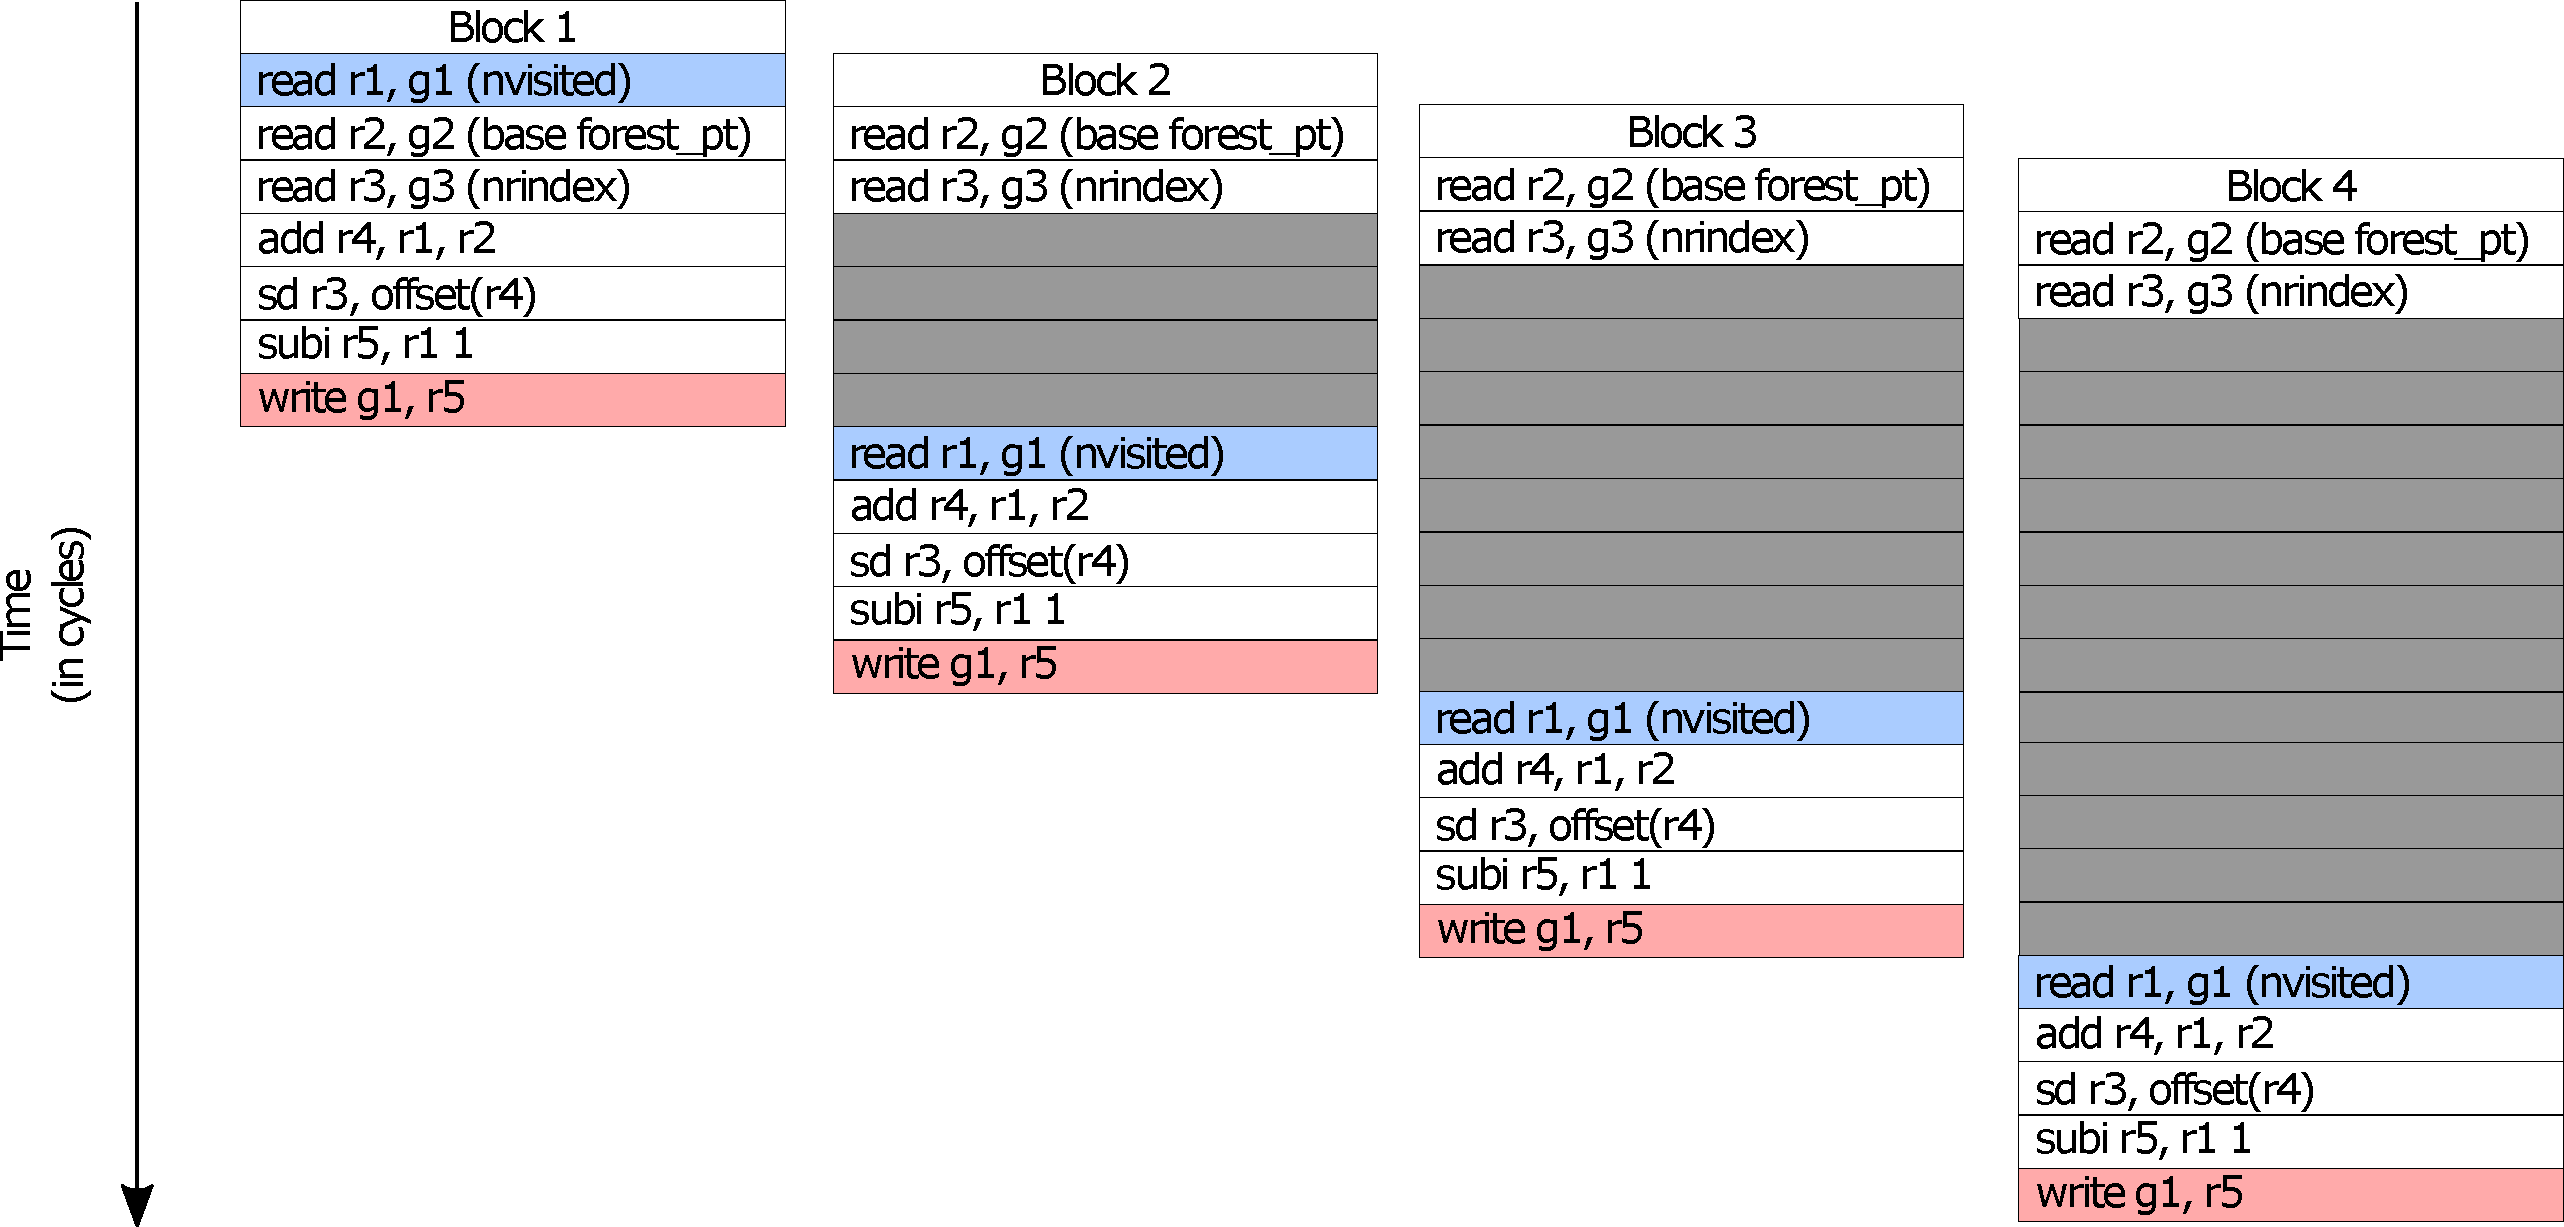
\includegraphics[width=1\textwidth]{chapter3/graphics/mser_ex.pdf}
		\captionof{figure}{Example of how data-dependencies cause delays when executing four blocks in parallel. The numbers represent part of the loop body in Listing~\ref{lst:mser_snipet}.}
    \label{fig:mser_nvsited}
	\vspace{1em}
\end{figure}

%If multiple blocks representing Listing~\ref{lst:mser_snipet} are in flight, the youngest block reading the value of \textit{nvisited} will have to wait for the previous block to execute the write.
%In such a case, a data dependency arises when executing multiple blocks in parallel if a write to a register which has to be read by multiple blocks is pending.
%This can be especially problematic when large core compositions are used, as up to 64 blocks can potentially be in flight at any moment.

To illustrate the data-dependency problem, Figure~\ref{fig:mser_nvsited} shows a simplified view of four blocks representing the body of the loop in Listing~\ref{lst:mser_snipet} being executed in parallel.
Each block starts executing a cycle after its parent; the instructions highlighted in colour represent the register causing the data-dependency; blue represents the register being read, and red represents the register being written to.
The grey slots represent cycles where the block cannot execute any instructions.
Assuming each instruction takes a single cycle to execute, 22 cycles are needed to execute all four blocks in parallel, compared to 28 cycles if they were to be executed sequentially.
If the data dependencies are not resolved quickly enough, then this causes blocks to execute in a serial fashion, which reduces any benefit from using the composition.

\begin{figure}[t]
    \centering
    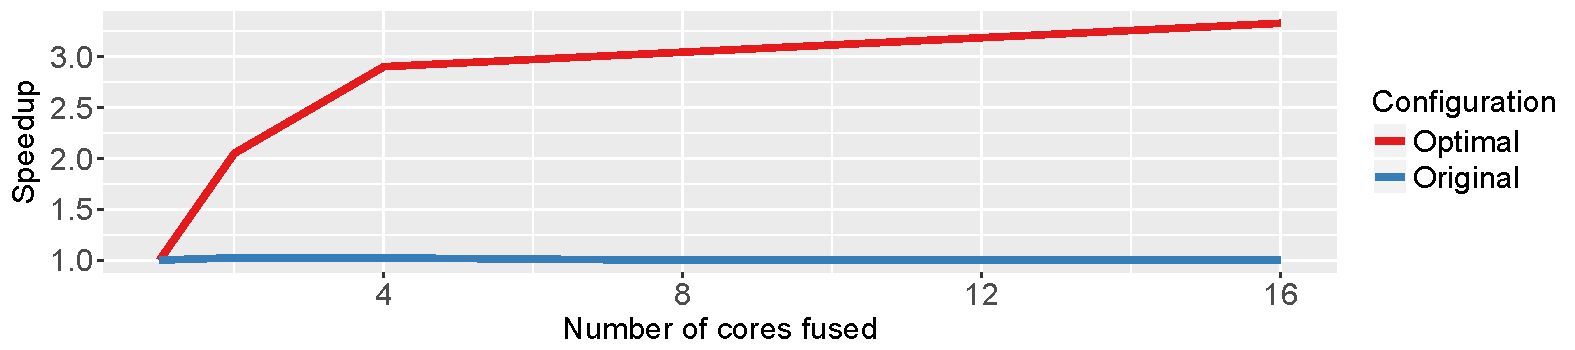
\includegraphics[width=0.95\textwidth]{chapter3/graphics/mser_motiv_reg2.pdf}
    \caption{Speedup of executing \bm{MSER} using the new fetching mechanism, with perfect value prediction and perfect branch prediction. Baseline is a single core with original branch prediction accuracy. Higher is better.}
    \label{fig:motivation_reg}
\vspace{1em}
\end{figure}


If cores do not have to wait on data dependencies, this can increase efficiency of core compositions, as they can execute their blocks independently.
Figure~\ref{fig:motivation_reg} shows how an optimal configuration of the processor, one that can fetch blocks in parallel, has perfect branch prediction and can immediately resolve data dependencies can improve performance on \bm{MSER}.
The speedup is obtained by comparing the execution time of core compositions to a normal single core, without perfect branch prediction.
The figure also shows the performance of a ``normal" core composition configuration that has no perfect branch prediction, serialised block fetches and cannot resolve data dependencies immediately.
As shown in the Figure~\ref{fig:motivation_reg}, a 16 core composition can now get a speedup of up to 3x, compared to the 2x when using only perfect branch prediction and the OF scheme.
%This is due to the fact that register dependencies are no longer serialising some of the computation between blocks, and thus blocks can be executed in parallel.

Serialised execution due to data dependencies is a common problem for superscalar processors~\cite{peraisVTAGE2014}.
One solution to the problem is adding a value predictor to the processor, which is able to predict the value of a register.
This allows instructions to execute with speculative data, and thus increase ILP and reduce the impact of data-dependencies.
Section~\ref{chp3:sec:val} covers the implementation of a value predictor for an EDGE processor which is used throughout this chapter.



%\subsection{Putting it all together}

%The previous 3 sections demonstrate that with modifications of the hardware, a previous benchmarks that showed very little performance gains with core composition can now see a performance increase of up to 1.90x on a 4 core composition.
%This demonstrates that the hardware used for core composition can be improved in order to tackle difficult applications.
%Whilst the previous three sections accumulated hardware modifications to obtain the 1.90x speedup, it is important to show how all these changes must be included in the processor in order to obtain the best results.

%\begin{figure}[t]
%    \centering
%    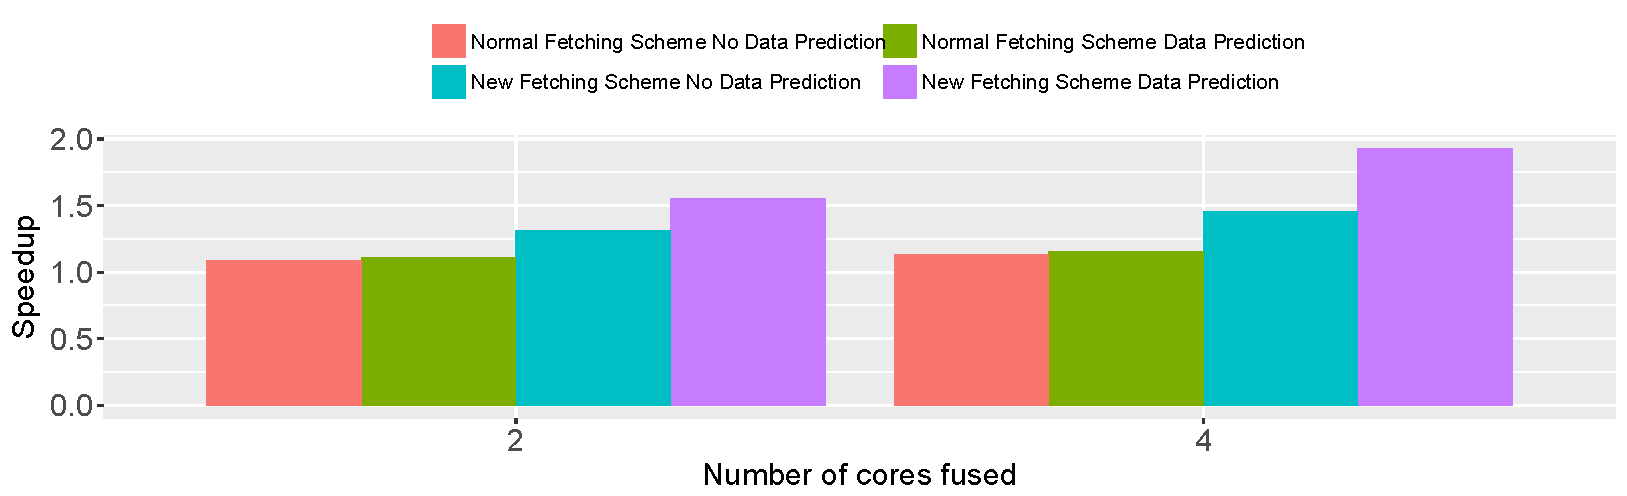
\includegraphics[width=1\textwidth]{chapter3/graphics/mser_final_motiv.pdf}
%    \caption{Speedup obtained when executing the MSER benchmark on 2 and 4 core composition with the new fetching scheme. Higher is better.}
%    \label{fig:motivation_final}%
%	\vspace{1em}
%\end{figure}

%Figure~\ref{fig:motivation_final} shows how the performance of \bm{MSER} is improved on when adding either the new fetching scheme, the value predictor, or both.
%The performance is compared to a single core with or without value prediction; all the experiments use a perfect branch predictor.
%Overall, the figure reveals that the current fetching scheme -- even with perfect value prediction and perfect branch prediction -- cannot obtain any significant performance improvements.
%This is due to the fact that the core compositions are limited by the serialisation of block fetches.
%Adding value prediction does not improve performance greatly because of the fact that it reduces the execution time of blocks, which once again increases the difficulty of populating cores with blocks.

%On the other hand, the figure also highlights that modifying the fetching scheme does not suffice in order to get the fastest execution times.
%%This is due to the fact that if cores are able to fetch blocks at a much faster rate, they will then be limited by potential register dependencies.
%Therefore, it is important to consider multiple modifications to the hardware in order to get the best performance.

%Finally, it is important to remember that these results are currently only made possible through the use of perfect branch prediction.
%Executing \bm{MSER} without perfect branch prediction leads to an average accuracy of 86\%, which is not enough to ensure that core composition can be efficiently used.
%This motivates exploring the potential performance of core composition through the use of a perfect branch predictor.

\section{Round robin block fetching scheme}\label{chp3:sec:fetch}

\lstset{
	backgroundcolor=\color{lbcolor},
	tabsize=2,
	rulecolor=,
	language=matlab,
        basicstyle=\tiny,
        upquote=true,
        aboveskip={1\baselineskip},
        columns=fixed,
        showstringspaces=false,
        extendedchars=true,
        breaklines=true,
        prebreak = \raisebox{0ex}[0ex][0ex]{\ensuremath{\hookleftarrow}},
        frame=single,
        showtabs=false,
        showspaces=false,
        showstringspaces=false,
        identifierstyle=\ttfamily,
        keywordstyle=\color[rgb]{0,0,1},
        commentstyle=\color[rgb]{0.133,0.545,0.133},
        stringstyle=\color[rgb]{0.627,0.126,0.941},
		numbers=left,
}


\begin{figure}[t]
\lstset{language=C,numbersep=4pt}
\begin{center}
\begin{lstlisting}
	for(int i =0 ; i < 100000; i++)
		a[i] = c[i]*b[i];
	
\end{lstlisting}
\end{center}
\vspace{-2em}
\captionof{lstlisting}{Example of small loop.}
\vspace{-1em}
\label{lst:basic}
\vspace{1em}
%\end{figure}

%\begin{figure}[t]
 %   \centering
 %   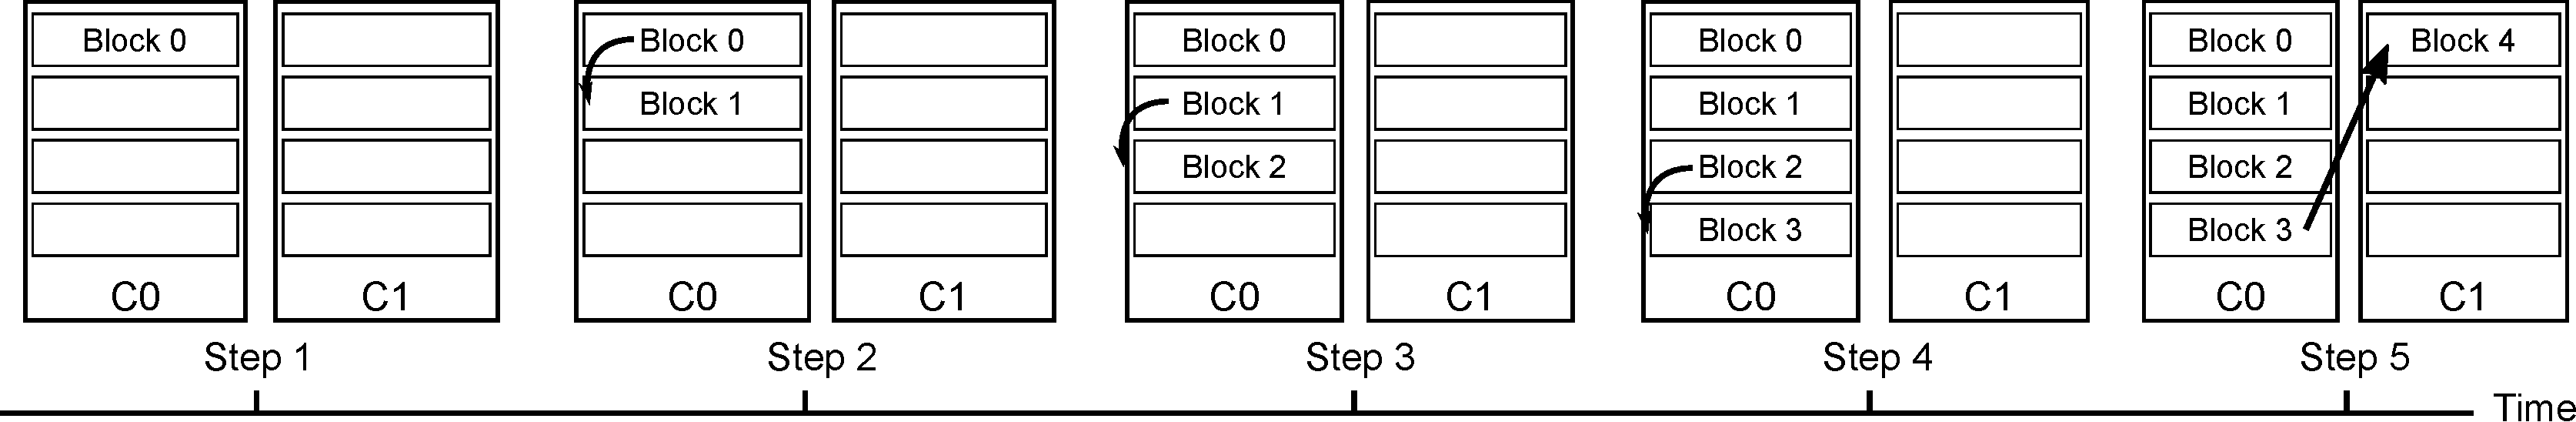
\includegraphics[width=1\textwidth]{chapter3/graphics/normfetch.pdf}
 %   \caption{Example of the current fetching model on a 2 core composition. Each core has 4 segments, the arrows represent the block generating the predictions.}
 %   \label{fig:old_fetch}
%\vspace{1em}
    \centering
    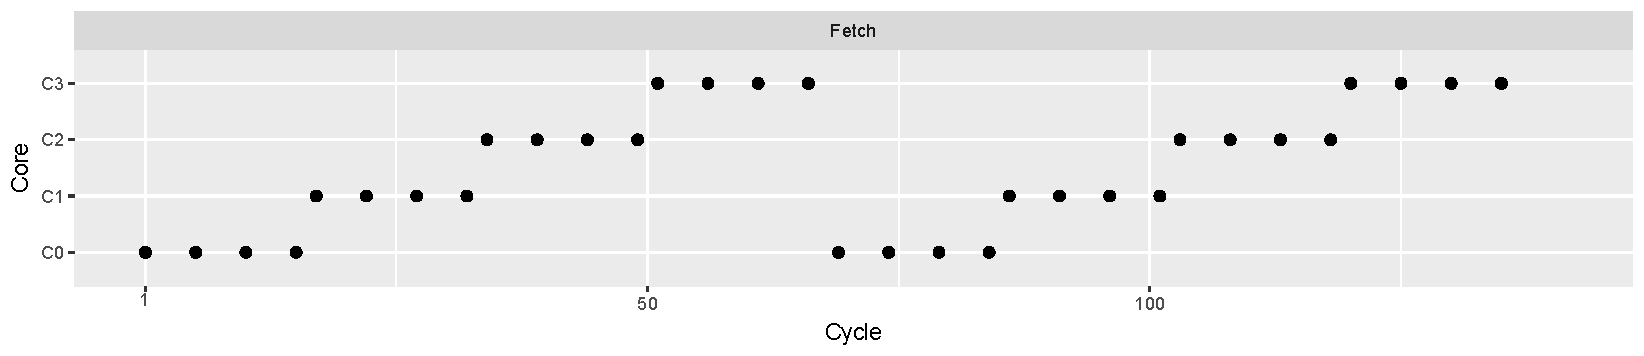
\includegraphics[width=1\textwidth]{chapter3/graphics/4fetchnorm2.pdf}
    \caption{Trace of when cores fetch blocks when executing Listing~\ref{lst:basic} on a 4 core composition. Y axis represents a core in the composition, X axis represents time.}
    \label{fig:fetch_norm}
\vspace{1em}
\end{figure}
\subsection{Current fetching scheme}
	
The main issue with the SF scheme is that cores in a composition depend on each other in order to fetch blocks.
For example, if Listing~\ref{lst:basic} is compiled without unrolling and executed on a 4 core composition, each core has to fetch 4 iterations of the loop before sending the next fetch request to another core.
To illustrate how fetching can be a bottleneck in this situation, instrumentation is added to the simulator to track when cores fetch blocks in order to be able to visualise how long it takes to fill up a core composition.
Figure~\ref{fig:fetch_norm} plots the when cores fetch blocks for a 4 core composition executing the code in Listing~\ref{lst:basic}.
Each point represents a block fetch, the X-axis represents the time (in cycles) whilst the Y axis represents which core has started fetching a block.
The figure shows that there are 50 cycles between the first block fetched by Core 0 and the first block fetched by Core 3.
Given that a block in Listing~\ref{lst:basic} takes only 10 cycles to execute, this means that Core 0 is inactive when Core 3 fetches.
This is due to the fact that once Core 0 submits a fetch request to Core 1, it will have to wait for Core 3 to send it a fetch request.

%Having a serialised block fetching scheme for core composition is one of the main bottlenecks for performance when the compiler cannot produce large blocks.
%This means that core composition is not an efficient method of executing small blocks in parallel, compared to using multithreading.
%When using multithreading, cores fetch blocks independently, thus maximizing throughput easily; the size of the block will not have the same impact on performance.
%A mechanism that alleviates fetch dependencies between cores is a first step in improving block throughput for core-compositions.

\subsection{Round Robin Fetching Scheme}

%Fetching blocks in a serial fashion currently makes large core compositions more difficult to use efficiently when blocks are small.
%Whilst serialising fetches aims to improve the efficiency of a single core by ensuring that its instruction window is full, it makes populating large core compositions a challenging task.
%If cores can fetch blocks independently, this allows larger core compositions to populate cores much quicker.

This section demonstrates how the fetching mechanism can be modified to allow for cores to fetch blocks in parallel.
It starts with a generalised version of the fetching algorithm for \textit{n} cores in a composition.
This is followed by a more in-detail example using a two core composition.
Finally it compares the performance of the new fetching scheme with the current fetching scheme on a synthetic benchmark.

\subsubsection{Generalised form}
The advantage of core composition is that multiple cores can execute the same thread.
Thus, the fact that the SF scheme prioritises filling a single core before using another core in the composition is counter-intuitive as it reduces the chance that all the cores are in use.
The new fetching scheme has two design objectives: reduce the number of times core's depend on each other to fetch blocks and ensure that each core in the composition is always executing at least one block.
Sequential blocks should not be found on the same core, instead they should all be on separate cores and fetched in a round robin fashion.
This ensures a more equal distribution of work amongst all the cores in the composition, and reduces the overhead of ensuring each core has a block.

%Currently, if a core does not have a block in its instruction window, it waits until another core in the composition sends it a fetch request.
If blocks are distributed equally amongst all cores using a round robin model, this new model still requires that each core must submit a fetch request to the next core.
This means that changing the fetching scheme to a round robin scheme does not necessarily stop cores from depending from one another to fetch blocks.
However, once a core has a block it can use branch prediction to predict the next block it must fetch, rather than waiting for another fetch request from a core.
As this new fetching mechanism employs a round robin scheme, the branch predictor must predict a block that is multiple steps into the future rather than the immediate branch.
By allowing cores to fetch blocks in \textit{strides}, instead of sequentially, the new fetching mechanism not only ensures cores have an equal amount of work, but that they can fetch in parallel.

\begin{algorithm}

\textbf{n} = Number of cores in the composition\\
\textbf{Composition[n]} = Core Composition Array\\
\textbf{branches[2]} = Branch Predictions for current block\\

\While{Program is Executing}
{
\Comment{Do branch prediction for up to 2 blocks}
branches = prediction[i+1, i+n]\\
\Comment{If the predictor generated 2 predictions}
\eIf{size(branches) == 2}
{
\Comment{If next core in composition is empty submit block i + 1 to it}
	\eIf{empty(Composition[currentPosition+1])}
	{
		submitToNextCore(branches[0])\\
		
		\eIf{myCore.full() == false}
		{
			submitToMyself(branches[1])
		}
		{
			buffer.push(branches[1])\\
		}
	}
	{
	\eIf{myCore.full() == false}
	{
		submitToMyself(branches[1])\\
	}
	{
		buffer.push(branches[1])\\
	}
	
	}
}
{
\Comment{If only block i + 1 prediction is valid}
	\If{empty(Composition[currentPosition+1])}
	{
		submitToNextCore(branches[0])\\
	}
}	
}
\caption{Overview of fetching algorithm for \textit{n} cores fused}~\label{alg:fetch}
\end{algorithm}

\begin{algorithm}
\textbf{n} = Number of cores in the composition\\
\textbf{Composition[n]} = Core Composition Array\\

\While{Program is Executing}
{
	\If{block is committing}
	{
		Composition[currentPosition+1] = Non Speculative\;
	}
	\If{not IsBlockRunning(Composition[currentPosition+1], block+1)}
	{
		submitToNextCore(block+1 PC)
	}
	
	\If{buffer.size() \textgreater{} 0}
	{
		fetch(buffer[0])
		buffer.pop()
	}
	\Else
	{
		Idle
	}
}
\vspace{-1em}
\caption{Overview of commit stage for \textit{n} cores fused}~\label{alg:commit}
\end{algorithm}

\paragraph*{Fetching mechanism}
Algorithm~\ref{alg:fetch} explains how the new fetching scheme, named Round Robin Fetch (RRF) works for \textit{n} cores in a composition.
In the general case, when a core composition is created, each core, aside from the core that initiated the composition, is empty.
When a core fetches a $block_i$, if the next core is empty, it makes two branch predictions, one for $block_{i+1}$ and one for $block_{i+n}$.
The predictions do not have to be done on the same cycle, however previous work on multi-block ahead branch predictors demonstrated that two predictions per cycle is possible~\cite{SeznecMultipleBlock}.
The core submits a fetch request to the next core in the composition for $block_{i+1}$ and then uses the prediction $block_{i+n}$ to fetch its next block.
If the next core is not empty, then the current core simply predicts $block_{i+n}$.

In case that a core cannot predict $block_{i+n}$, it simply submits a prediction for $block_{i+1}$ to the next core.
The core will then have to wait for another core in the composition to send it the prediction for $block_{i+n}$.
Whilst this case may impact overall throughput, it is no different than the SF scheme as SF would also stop fetching after $block_{i+n-1}$ and wait for $block_{i+n}$'s PC to be resolved.

In the SF scheme, when a core is full, it submits a fetch request to another core in the composition by sending the address of a block to a buffer found on that core.
To ensure cores are always fetching blocks in RRF, the buffer is used when a core has filled up its instruction window and can no longer fetch blocks.
Instead of sending the fetch request to another core, a core saves the block address in its own buffer, and will handle that fetch request once it has committed a block.
In this chapter, a core can only have one buffered PC at a time.

\paragraph*{Committing mechanism}
Algorithm~\ref{alg:commit} shows how blocks are committed in RRF.
When committing $block_i$, the core sets the next core in line to be the non-speculative core.
This is due to the fact that that core will always have $block_i+1$.
If the next core in line does not yet have $block_{i+1}$ due to no prediction having been made, then the committing core will submit the resolved PC to the next core, rather than fetching it for itself.
If the core has a PC in its buffer, it immediately starts fetching a new block.
However, if it has no PC in its buffer, it must wait on another core to send it a request.

\begin{figure}[t]
    \centering
    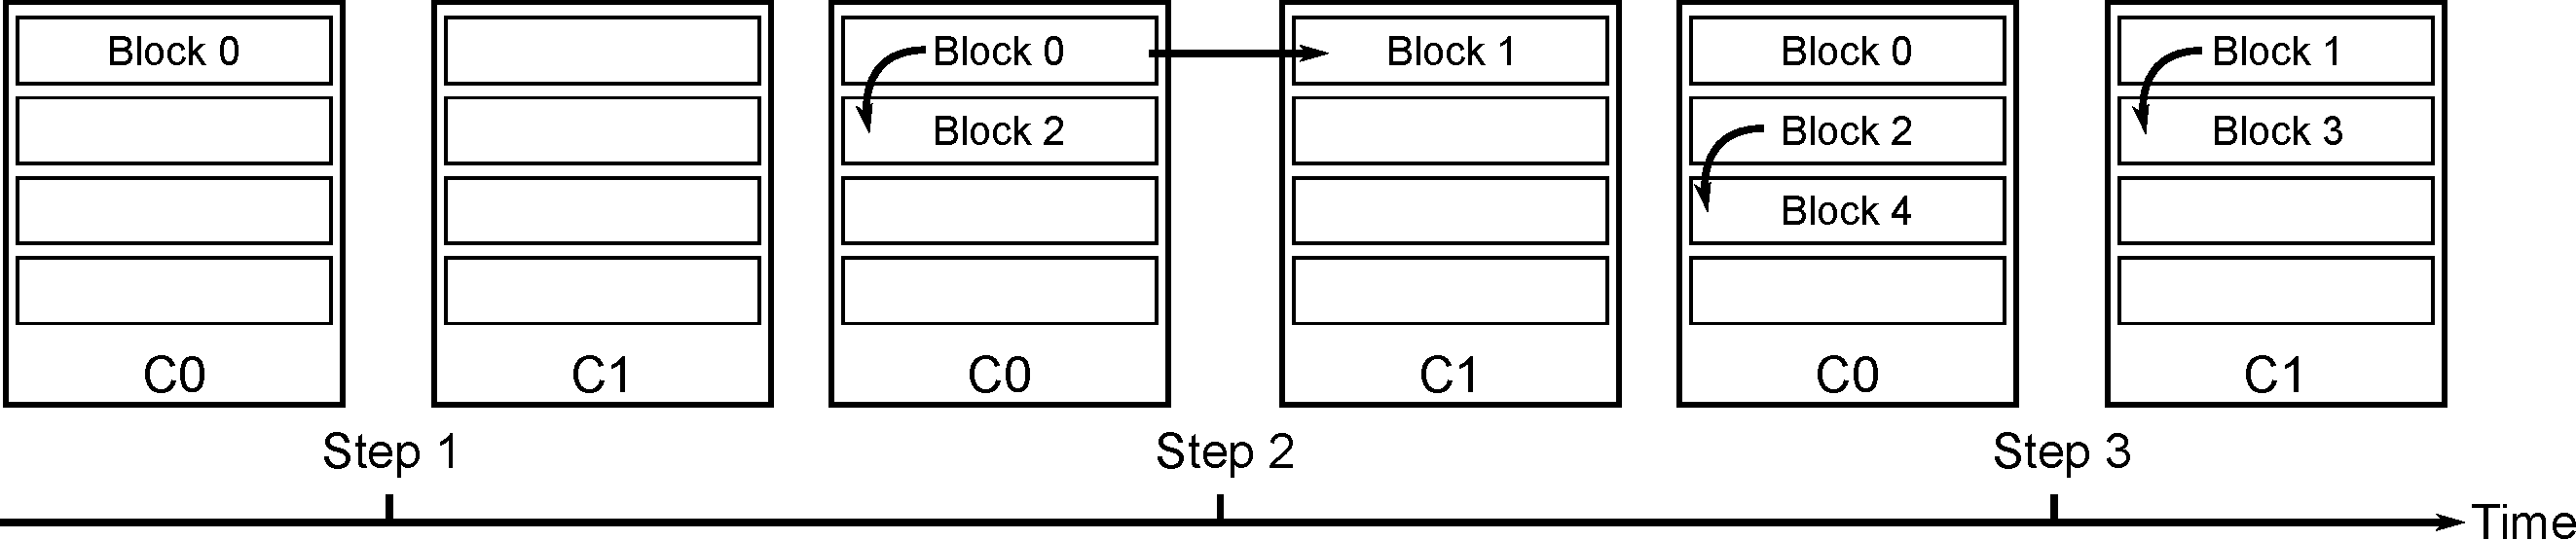
\includegraphics[width=1\textwidth]{chapter3/graphics/fetching-model.pdf}
\vspace{-2em}
    \caption{Example of RRF on a 2 core composition. Each core has 4 segments, the arrows represent the block generating the predictions.}
    \label{fig:new_fetch_ex}
	\vspace{1em}
\end{figure}
	
\paragraph*{Two core example}
	
%Given a 2 core-fusion \{$Core_0$,$Core_1$\} using a ITTAGE~\cite{SeznecITTAGE} multi-block ahead branch predictor described by A. Seznec et al in~\cite{SeseznecMultipleBlock} the cores can make two predictions in a single cycle: one for itself and one for the next core.
Figure~\ref{fig:new_fetch_ex} gives an overview of the first few cycles of using RRF with two cores fused.
When $Core_0$ starts the composition and fetches the first block, $block_0$, if it is able to predict $block_2$ will submit a fetch request for $block_1$ on $Core_1$ whilst also attempting to fetch $block_2$ for itself.
On the next cycle	e $Core_1$ receives the request for $block_1$ and starts fetching the block.
Once $Core_1$ can make a branch prediction it will attempt to predict for $block_3$ instead of $block_2$; this is because $block_2$ was already predicted and fetched on $Core_0$.

%In this new fetch mechanism, when a core is in fetching mode, it does not attempt to predict $block_{n+1}$ but rather $block_{n+numberOfCoresInComposition}$; the reason behind this will be clarified shortly.
%If $Core_0$ or $Core_1$ attempts to fetch a block when it is full, it can submit the new block's PC to a buffer; the core then stops attempting to allocate new blocks.
%Once the full Core has committed a block, it checks if it has a buffered PC, and if it does it fetches that block.

%As long as $Core_0$ and $Core_1$ can fetch and predict blocks correctly, they will fetch in a pipelined fashion.
%This means that $Core_0$ will have blocks \{0,2,4,6\} whilst $Core_1$ has \{1,3,5,7\}.
%The reason behind this is to minimize the Synchronization Cost defined in Chapter 2 as now each Core will be committing a block in turn.

%In the case that $Core_0$ cannot make a prediction for $block_2$ it will only send a fetch request for $block_1$ to $Core_1$.
%When this happens, $Core_0$ will no longer be able to fetch blocks until it is sent a PC from $Core_1$.
%The request will happen once $Core_1$ commits $block_1$ and the PC of $block_2$ is resolved.
%Whilst this case may impact overall throughput, it is no different than the current model as the current model would also stop fetching after $block_1$ and wait for $block_2$'s PC to be resolved.

\paragraph*{Limitation}

Whilst RRF allows for cores to fetch out of order in parallel, blocks must still be dispatched in order.
This is to ensure that blocks do not execute data-dependent register reads out of order, when dependencies are not yet determined.
To achieve this, each core maintains a flag that tells it whether or not its oldest - not yet dispatched block - can be dispatched.
Since blocks are fetched in a round-robin fashion, whenever a core starts dispatching a block, it sets the flag to false, and informs the next core to start fetching.
Only a single core has this flag set to true, thus insuring blocks are dispatched in order.
In this chapter, compositions are created out of cores that are physically close, and the following block is always on a core that is 1 network hop away (1 clock cycle).
Assuming, for this architecture, that a hop takes a single cycle, a block can theoretically be dispatched every cycle.

%To achieve this, a record of the last dispatched block number is kept in a shared counter.
%When a block tries to dispatch instructions it checks the counter, if its block number is sequentially next then it atomically updates the counter to the value of its block number and dispatches its block.

%This mainly impacts the performance of large compositions when the system is not in a steady-state of fetching and dispatching blocks and the blocks are small.
%This is due to the fact that the fetch stride is larger and thus cores will have to wait longer for blocks on other cores to dispatch.
%For example, when starting a composition of 16 cores, the first core will have blocks 1 and 17 in its instruction window.
%However, it will have to wait on all other cores to fetch a block before dispatching block 17, which may take 60 or more cycles.

%This limitation could be alleviated by creating a more complex fetching scheme that takes into account which cores are available to fetch and dispatch blocks immediately, rather than having a stride that is fixed ahead of time.
%Such a scheme may require to centralise the fetching though, as it would require more awareness of what each core is executing.
%Centralising the fetching mechanism increases the pressure on the network as each core will have to send a block PC to the scheduler, and the scheduler will then have to re-submit that PC to an available core.
%This is twice as many network messages per block compared to SF and RF.
%The implementation of a centralised fetching scheme is not explored throughout this Chapter, yet it is suggested as future work.

\subsection{Evaluating the round robin fetch scheme on a synthetic block}

\begin{figure}[t]
    \centering
    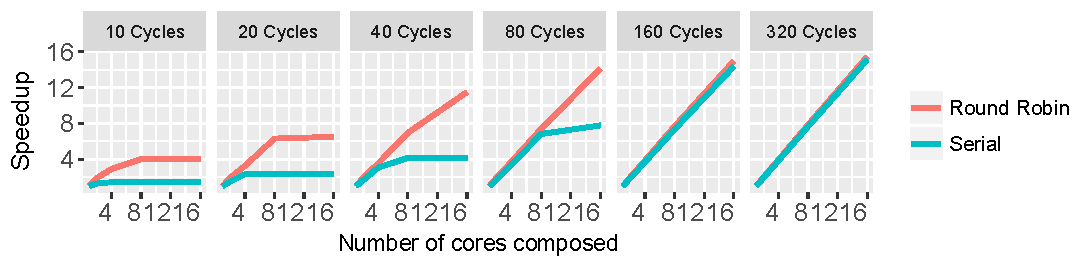
\includegraphics[width=1\textwidth]{chapter3/graphics/motivation_fetch2.pdf}
   	\vspace{-2em}
 \caption{Speedup when executing the synthetic block with varying execution times (facets) with SF and RRF. Higher is better.}
    \label{fig:motiv_res}
    \centering
    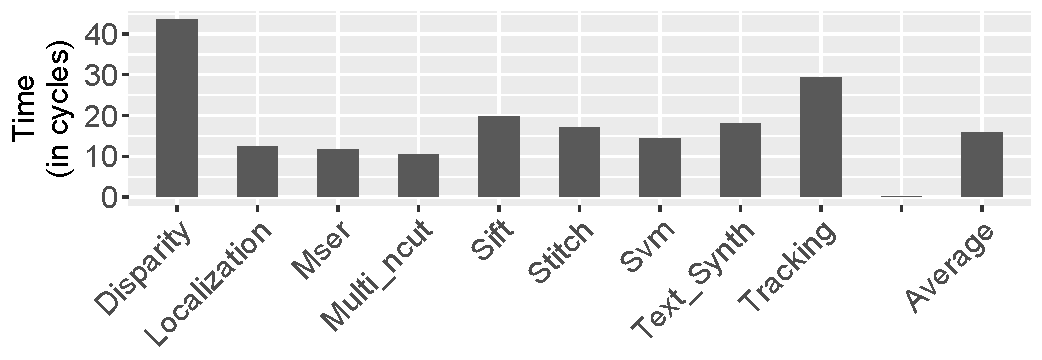
\includegraphics[width=1\textwidth]{chapter3/graphics/sdvbsav.pdf}
    
	\vspace{-0.5em}
	\caption{Average execution time (in cycles) of blocks for each of the SD-VBS benchmarks. Each benchmark was executed on a single core with a single lane with perfect branch prediction.}
	
    \label{fig:svdbs_av}
\vspace{1em}
\end{figure}

Before evaluating the performance of RRF on a set of benchmarks, it is important to measure the potential performance increase on a simpler case.
This is due to the fact that other factors than the size of blocks, such as data-dependencies, cache misses or load-store queue violations can affect the performance of a composition.
Therefore, evaluating the new fetching scheme on a synthetic benchmark can provide a ceiling for the maximum performance gains when using RRF.

For this section the synthetic block is only four instructions long using a custom instruction whose execution time is defined ahead of the simulation.
The reason a four instruction block was chosen is due to the fact that it allows for four blocks to be fetched on each core, which is the worst-case scenario for the SF scheme.
Whilst the SF scheme is susceptible to small blocks, the main issue is when these blocks execute quickly, as it means that the composition cannot be filled.
On the other hand, if a block is small yet hundreds of cycles to execute, for example due to multiple cache misses, then the SF scheme would still perform fine, as filling cores would take less time than executing blocks.
This is why the execution time of the block is variable, as it allows to cover different cases.
For this experiment, six different execution times are explored: $Exec=\{10,20,40,80,160,320\}$.

Figure~\ref{fig:motiv_res} shows the speedup obtained when using core composition when executing the synthetic benchmark, with the SF or RRF scheme with a baseline of a single core.
The facets represent the different execution times of the block whilst the colours represent the different fetching schemes.
The results in the figure show that unless a block is at least 80 cycles long, it is difficult to efficiently use 16 core compositions using SF.
To give a point of reference -- with data gathered from the SD-VBS benchmarks from Chapter~\ref{chp:cases} -- the average execution time (in cycles) of a block for each of the SD-VBS benchmarks is displayed in Figure~\ref{fig:svdbs_av}.
The figure shows that, on average each block in a benchmark only takes 15 cycles to execute, with \bm{Disparity} having the longest blocks with an average of 40 cycles.
With the new fetching scheme, 16 cores becomes useful when blocks are at least 40 cycles long, enabling a 3x speedup compared to the old fetching scheme.
%For smaller core compositions, such as 2 and 4 fused cores, using a different fetching scheme from the traditional method allows for core composition to speedup execution when blocks are even 10 cycles long.

\section{Value Predictor}
In an EDGE block, data dependent instructions do not pass data to each other via reads and writes to registers, instead the result of an instruction is passed to the operands of instructions who depend on the data (see Chapter~\ref{chp:Background} for more information).
Registers are primarily used to pass information between blocks.
In a core composition the register files of each core in the composition is shared (Chapter~\ref{chp:Background}) to ensure that each core has the same view of the current execution state.
When the register files are shared each core becomes responsible for a set of registers; for example in a 2 core composition, the even numbered registers are handled by Core 0 whilst the even number registers are handled by Core 1.
This means that when Core 1 wants to read or write to Register 0 it must send a request via the network on chip (NoC) as this register is located on Core 0.

\begin{figure}[t]
\lstset{language=C,numbersep=4pt}
\begin{center}
\begin{lstlisting}
	for(int i =0 ; i < 100000; i++)
		a[i] = c[i]*b[i];
	
\end{lstlisting}
\end{center}
\vspace{-1em}
\captionof{lstlisting}{Example of small loop.}
\label{lst:basic2}
\vspace{3em}
\end{figure}

As the register reads found in blocks are hardcoded, this means that a single core may receive many register requests per cycle.
For example, the base address of the arrays in Listing~\ref{lst:basic2} are going to be passed via 3 registers in the block that represents the body of the loop.
If this loop is executing on a 16 core composition, then 3 of the cores will have to issue all the reads to these 3 registers for all other cores.
This of course will put stress on the NoC, and increase the latency of what is meant to be a relatively fast instruction.

To ensure that a younger block does not execute a read to a register that must be written to by an older block, the register-file keeps track of registers which will be written to by older blocks.
If the younger block attempts to execute the read, its request is pushed back until the older block has executed its write and any instruction that depends on the read must wait until the write fires.
Whilst the serialisation of register reads and writes between blocks ensures correct execution of speculative blocks, it effectively reduces the potential for instruction level parallelism (ILP).
This is further exacerbated when fusing a large number of cores, as this increases the amount of blocks that may potentially have to wait on register reads and writes.

For example, the loop iterator in Listing~\ref{lst:basic2} is passed between iterations of the block through a register.
If multiple cores are composed, and all have an iteration of the loop, they may have to wait on previous writes to be able to execute their loads; serialising execution of the loop.
In situations where register dependencies are a bottleneck and cannot be optimised via a compiler, core composition cannot be considered an effective method of improving performance as the data dependencies serialise execution of blocks.

This chapter underlines two problems related to register reads on large compositions: the potential data dependencies caused by reads waiting for previous writes to execute, and the latency caused by having to send read requests via the NoC.
The problem of trying to reduce register and memory dependencies to improve instruction level parallelism is not new, and is an issue found in more traditional superscalar processors~\cite{peraisVTAGE2014}.
For example, in the loop of Listing~\ref{lst:basic}, the sole data dependency is found in the loop induction variable.
This variable is always incremented by 1, which means that given a block, the value can easily be predicted based on previous values of the variable.
The other register values, such as the memory bases can also be predicted as they never change.
If each core is able to predict the value of the register reads, then they can speculatively execute instructions that depend on these registers before the real value arrives.
In these cases value prediction can be used to attempt to ensure that these blocks can run in parallel even if there are dependencies.

\begin{figure}[t]
    \centering
    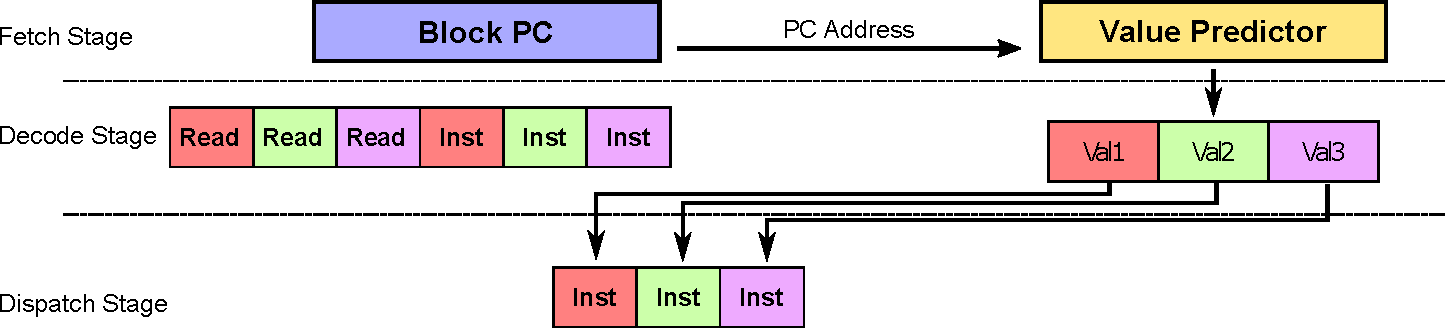
\includegraphics[width=1\textwidth]{chapter3/graphics/val_pred_overview.pdf}
    \caption{Overview of how a value predictor should work for EDGE. Prediction is made at the fetch stage, and predictions are used when register reads are dispatched.}
    \label{fig:bad_overview}
\vspace{1em}
\end{figure}

\subsection{Design features of a value predictor}

In this chapter, the only target for value predictions is register read instructions.
This is due to the fact that other instructions do not depend on previous blocks to fire, and load/store instructions can be fired independently unless dependencies are predicted.
Ideally, a value predictor for EDGE would function as seen in Figure~\ref{fig:bad_overview}.
When a block is fetched, a single request is made to the value predictor to fetch all predictions for the read instructions of the block.
At dispatch time, the predicted values would be used and forwarded to instructions depending on a read, whilst the read instructions are issued.
This allows the depending instructions to execute whilst the reads are still being processed.
This section covers different features that must be considered when implementing such a value predictor.


\paragraph*{Prediction Latency}
In a traditional superscalar processor, one of the main challenges value predictors face is being able to sustain the potential number of prediction requests in a short time frame~\cite{peraisBeBop2015}.
As value predictors are designed to improve ILP performance of out-of-order (OoO) superscalars, it is important to be able to issue a predicted value quickly.
If multiple prediction requests are made each cycle, this may require xpensive hardware such as a re-order buffer to hold all predictions~\cite{peraisBeBop2015}, which may dissuade designers from using value predictors.

To tackle the challenge of issuing predictions quickly, research has focussed on grouping instructions into prediction blocks~\cite{peraisBeBop2015}.
Instead of fetching a single prediction, each entry in the value predictor represents a set of predictions.
Entries are accessed by using the PC of the first instruction in a fetch block.
By grouping multiple predictions into a single entry, it drastically reduces the amount of requests to the value predictor, reducing the prediction latency for a large amount of instructions.
However, a block-based value predictor requires that the size of a block be determined at design time, which adds a new design task: choosing a small block size will increase the number of requests per cycle, whilst a large block size will decrease the number of entries and thus reduce overall accuracy.
As EDGE organises instructions as blocks, a block-based predictor would reduce the number of prediction requests per cycle, making it an attractive feature.


\paragraph*{Prediction generation} Another important feature when selecting a value predictor is how it generates a predicted value.
As of the writing of this thesis, there exist two main methods: direct value prediction~\cite{peraisVTAGE2014} and stride-based value prediction~\cite{peraisBeBop2015,gabbayVPOrig,goeman01dfcm}.
The direct value predictor is the simpler design, as it only stores the last retired value for the specific instruction.
When a request is made, the direct value predictor will simply submit the last value.
Whilst this makes a value predictor small easy to design, such implementation is known to have poor accuracy when predicting values that are modified in quick succession.

On the other hand, stride-based value predictors use two components to make a prediction.
The first component is a Last-Value Table (LVT) which holds the last retired value for the instruction.
The second component is a stride, which represents the delta between the last two retired values for the instruction.
When a prediction is made, the value predictor fetches the value from the LVT, and adds the stride to make a prediction.
Such a design may increase the memory footprint as it has to store both a value and a stride for each data point; however it improves the overall accuracy and usefulness of value predictors.
It is also more accurate when executing loops as it can detect the stride at which the register values are modified.
As core composition is best used when executing loops, a stride-based predictor is recommended.

\paragraph*{Summary}

A perfect value predictor for EDGE must therefore be able to provide predictions in groups, as EDGE organises its instructions in blocks as this reduces the number of prediction requests per cycle.
Also, as value prediction is to be used in core compositions, a stride-based predictor is more adequate than a context based one.
Perais et al. propose such a predictor: a block based differential Value TAGE predictor~\cite{peraisBeBop2015}.
The next section covers briefly how this predictor works.

\subsection{Block based D-VTAGE predictor}

In this chapter, a block based differential value TAGE (D-VTAGE) predictor is implemented, based on the work of Perais et al.~\cite{peraisBeBop2015}.
Full details on how such a value predictor works can be found in Chapter~\ref{chp:Background} Section~\ref{chp:bck:vtage}.
To summarise, D-VTAGE is a stride based value predictor, which means that a prediction is composed of the last seen value for the instruction (found in a Last Value Table (LVT)), and a stride which represents the delta between the last two values for the instruction.
When a prediction is made, the last seen value and stride are added together to make the predicted value.

The predictor must also handle the fact that multiple blocks may be in flight, and thus the value found in the LVT may not be up to date.
In order to handle multiple in-flight predictions, D-VTAGE also contains a speculative window that has its own LVT that is speculatively updated when new predictions are made.
This allows the predictor to be able to handle situations where mutliple iterations of a loop are in flight.

Instead of issuing a single prediction per request, the block based D-VTAGE predictor issues multiple predictions for a single request.
This is an ideal mechanism when considering EDGE is the targetted platform.
In this case, when an EDGE block is fetched, a single request has to be made to the predictor to fetch all predictions for register reads.

Finally, as EDGE blocks are single entry, multiple exits, this simplifies the update mechanism for the Speculative Window.
In the original proposal of D-VTAGE by Perais et al.~\cite{peraisBeBop2015} they discuss the issue of how to handle updates in the Speculative Window after a flush.
This is due to the fact that in a traditional x86 environment, instructions being fetched after a flush may belong to a block of instructions that initiated the flush.
As this is not possible in EDGE, since whole blocks are flushed and fetched, there is no need for a complicated update policy.
Instead, a new prediction is always made when a block is fetched.



%\subsection{Perfect Value Predictor}

%The perfect value predictor is implemented using traces of the application being executed.
%When a new block is fetched, it querries the trace file and looks for the values of all the registers which will be read.
%When the block can execute a read, the simulator then feeds the register directly into the instruction operands, instead of querying the register file.

%The perfect value predictor has no hardware restriction as to fully capture the potential performance improvements.
%Thus, all the registers in a block can be predicted.
%More on how restricting the number of values which can be predicted per block is discussed in the analysis in Section~\ref{chp:chp3:sec:analysis}.
\label{chp3:sec:val}
\section{Experimental Setup}
\subsection{Benchmarks}
To evaluate how the hardware modifications improve the performance of core composition; the same benchmarks used in Chapter~\ref{chp:cases} are used here.
These benchmarks are all from the San-Diego Vision Benchmark Suite (SD-VBS)~\cite{sdvbs}, which is composed of a set of vision and image analysis applications, and are described in detail in Chapter~\ref{chp:setup} Section~\ref{chp:setup:sdvbs}.
The previous chapter showed that even with code optimisations, core compositions do not perform optimally when executing the benchmarks.
Some of the programs, such as \bm{MSER} or \bm{Multi\_NCut} features an average block size of under 10 instructions, making it difficult to use core composition efficiently.
They are therefore a perfect candidate to explore how the hardware modifications can improve the performance of core composition.

\begin{table}[t]
  \smaller
  \centering
 \begin{tabular} {| l | l | l | l | l | l | }
 \hline
   & \cellcolor[gray]{0.7}Disparity & \cellcolor[gray]{0.7} Localization& \cellcolor[gray]{0.7} MSER& \cellcolor[gray]{0.7} Multi\_NCut& \cellcolor[gray]{0.7} Sift\\ \hline
Input&	VGA  & VGA & CIF  & SIM\_FAST& CIF\\ \hline
	
	 & \cellcolor[gray]{0.7} Stitch & \cellcolor[gray]{0.7} SVM & \cellcolor[gray]{0.7} Text. Synth & \cellcolor[gray]{0.7} Tracking&\\ \hline
	  Input & CIF& CIF& FULLHD& VGA &\\ \hline

	\end{tabular}
  \caption{Datasets used for each of the benchmarks.}\label{tab:sd-data2}
\vspace{1em}
\end{table}
\subsection{Evaluation} 
The previous chapter showed that the SD-VBS benchmarks feature repeating phases of IPC.
These benchmarks are structured as pipelines with distinct passes that are often repeated.
This means that performance improvements can be analysed without having to fully execute the program.

As this chapter is only concerned with demonstrating that the new hardware modifications outperform the current implementation, the benchmarks are executed long enough to capture all the phases.
The phase data gathered from Chapter~\ref{chp:cases} is used to determine hot-spots.
The benchmarks are then instrumented so that the main phases are captured, and executed for at least 100 million instructions.
Of that 100 million instructions, 10 million instructions are for warming up the caches and predictor whilst the rest are used to record performance.
Finally, the same data-sets from Chapter~\ref{chp:cases} are used, to maintain a consistency amongst the thesis; they can be found in Table~\ref{tab:sd-data2}.

\subsection{Value Predictor}

Value predictors that generate predictions both quickly and accurately are still actively being researched~\cite{peraisVTAGE2014,peraisBeBop2015,sheikh2017value}.
In order to motivate the use of value prediction for core composition, it is first important to abstract away current implementation details of state of the art predictors.
By considering a 100\% accurate prediction rate and immediate value prediction, this helps to determine how much value prediction can help improve performance.
Once the maximum speedup is determined, using a current state-of-the art implementation can help understand how far current value predictors are from the best performance.

This chapter explores two value predictors: a perfect value predictor that can predict any value in a single cycle, and a block based D-VTAGE~\cite{peraisBeBop2015} value predictor.
To have a better picture of how state-of-the art affects performance, different parameters of the predictor are modified.
This is discussed in further details in Section~\ref{chp:chp3:sec:analysis2}.

\subsection{Implementing perfect value and branch predictor}

\begin{figure}[t]
    \centering
    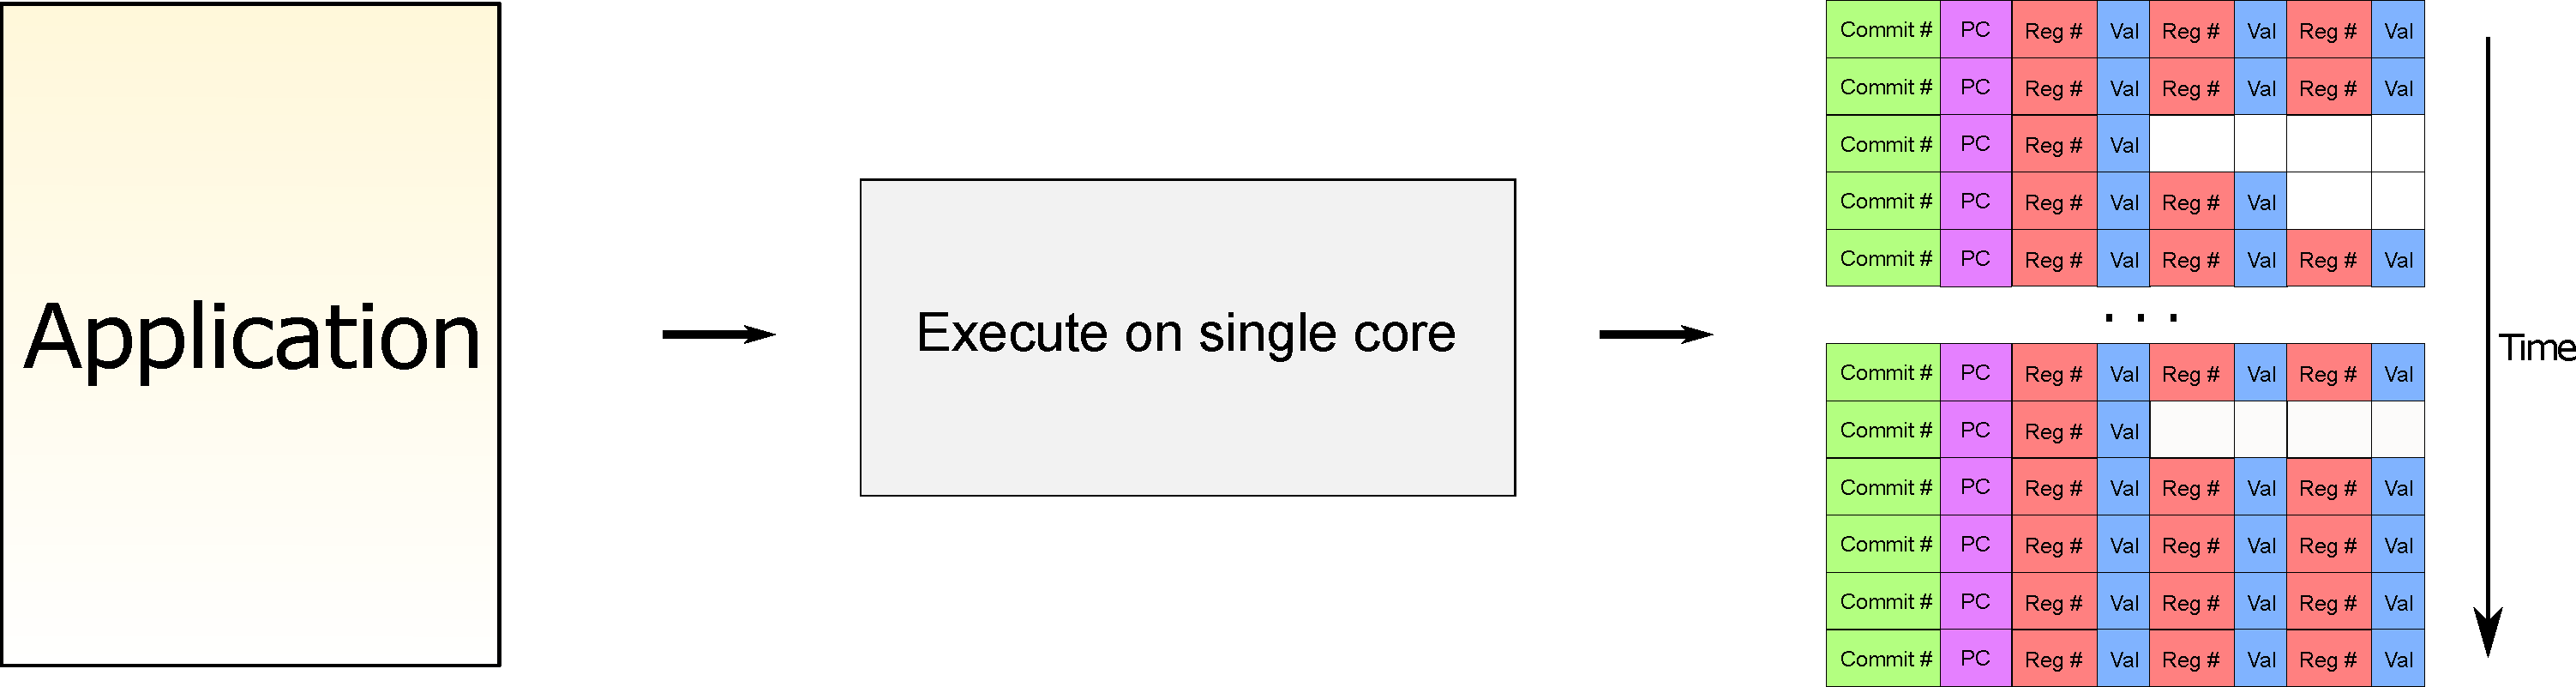
\includegraphics[width=1\textwidth]{chapter3/graphics/trace-gen.pdf}

    \caption{Overview of information gathering for generating traces which are used for the perfect branch and value predictors.}
    \label{fig:trace-gen}
\vspace{1em}
    \centering
    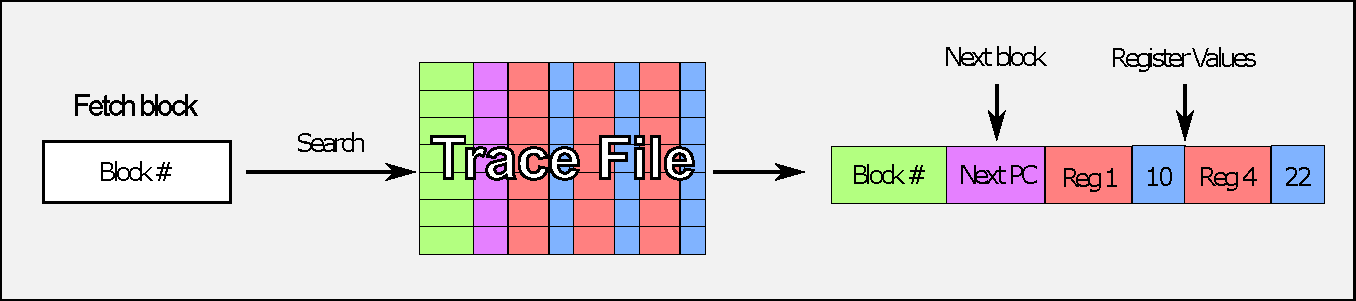
\includegraphics[width=1\textwidth]{chapter3/graphics/fetching-trace.pdf}

\vspace{1em}
    \caption{Overview of how the trace data generated for value prediction is used during execution of a block.}
    \label{fig:trace-used}
	\vspace{1em}
\end{figure}

This chapter is concerned with how changing the hardware will improve the performance of core composition.
In order to motivate new research in branch prediction and value predictors and their use for core composition, it is essential to know what the maximum performance improvements are when using these techniques. %they're not techniques but you get the idea.
Thus, a perfect value predictor and branch predictor are considered for the analysis.

These predictors use execution traces of each application to make their predictions.
Figure~\ref{fig:trace-gen} shows how these traces are generated.
The trace file contains an entry for every committed block, which is comprised of the Program Counter (PC) for the next block, a list of registers that were read and their corresponding values.

When the perfect predictors are activated, the simulator reads in the trace file.
Figure~\ref{fig:trace-used} shows how the trace data is used: a newly fetched block is paired with its correspondent trace data.
Instead of using the branch predictor, the next block's PC is directly taken from the trace entry, and whenever the block can issue a register read, the value is fetched from the trace entry instead of making a request to the register file.
\vspace{-2em}
\label{chp:chp3:sec:exp}
\section{Performance analysis using a perfect value predictor}
\newcommand{\novp}{\textit{\textbf{SFNoVP}}}
\newcommand{\vp}{\textit{\textbf{SFVP}}}
\newcommand{\nfnovp}{\textit{\textbf{RRFNoVP}}}
\newcommand{\nfvp}{\textit{\textbf{RRFVP}}}

\newcommand{\optvp}{\textit{\textbf{OptVP}}}
\newcommand{\vt}{\textit{\textbf{VT}}}
\newcommand{\nfvt}{\textit{\textbf{RFVT}}}
\vspace{-1em}

This section explores how a perfect branch and value predictor, paired with the new fetching scheme (RRF), improves the performance of core composition.
To understand how each component contributes to the performance improvements, different configurations were used, they are as follows:
\begin{itemize}
\item Serial fetching scheme with no value prediction (\novp).
\vspace{-1em}
\item Serial fetching scheme with perfect value prediction (\vp).
\vspace{-1em}
\item Round robin fetching scheme with no value prediction (\nfnovp).
\vspace{-1em}
\item Round robin fetching scheme with value prediction (\nfvp).
\end{itemize}

All configurations use perfect branch prediction  to ensure that core composition is always on the correct execution path.
All benchmarks are executed with 16 cores composed as this is the maximum number of cores that can be fused.
No dynamic adaptation is done as Chapter~\ref{chp:cases} showed that the primary advantage of dynamic core composition is energy savings, whereas this chapter focuses on speedup.


\subsection{Analysing the performance of the different configurations}
Figure~\ref{fig:perf_pred} shows the speedup obtained on the SD-VBS benchmarks using the different configurations.
The baseline for this section is 16 cores composed with serial fetch (SF) no value prediction (\novp) and perfect branch prediction.
This baseline is chosen as this chapter is focused on improving the performance of core composition.

First, it is clear that using RRF with value prediction (\nfvp) always results in the best speedup compared to the baseline.
For \bm{Multi\_NCut}, performance is improved by 3x when using \nfvp.
This is a significant speedup, as Chapter~\ref{chp:cases} showed that \bm{Multi\_Ncut} is a difficult benchmark for core composition (1.3x speedup in Chapter~\ref{chp:cases}).
On average, \nfvp{} outperforms the baseline by a factor of 1.88x.

\begin{figure}[t]
    \centering
    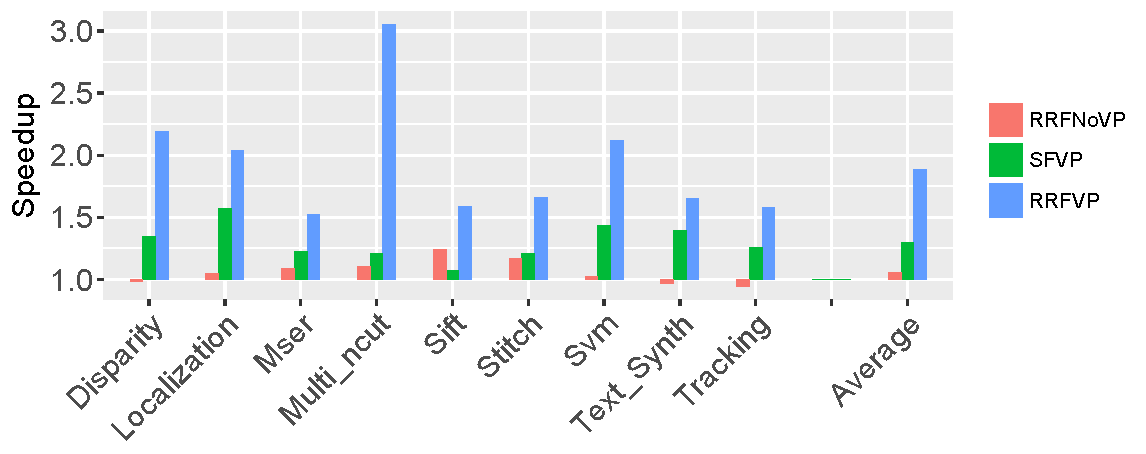
\includegraphics[width=1\textwidth]{chapter3/graphics/tempres4.pdf}
    \caption{Comparing the performance of serial fetch to round robin fetch, with and without perfect value prediction. Higher is better}
    \label{fig:perf_pred}
\end{figure}

\subsubsection{Performance without value prediction}
The results in Figure~\ref{fig:perf_pred} show that without value prediction the performance improvements brought by RRF on its own are low, or in fact detrimental to performance.
For example, \bm{Multi\_NCut} only has a 1.10x speedup when using the \nfnovp{} configuration, compared to the 3x of \nfvp{}.
This is due to the fact that whilst more blocks are now spread across cores, the register dependencies between blocks limit the performance of the composition. 
In fact, the more even distribution is the reason why some benchmarks perform worse: \bm{Disparity}, \bm{Texture\_Synthesis} and \bm{Tracking} see a slight performance decrease.
The even distribution of blocks amongst cores increases the stress on the network on chip (NoC) as more cores will make accesses in parallel.
Without value prediction, RRF suffers due to NoC stress and data dependencies.
%In fact, \vp{} outperforms \nfnovp{} on \bm{Localization}, which shows that register dependencies between blocks can make the new fetching scheme less performant than the currently implemented.

%The performance limitations are caused by blocks that are further down the speculative path that must wait for older blocks to write to the register file.


\subsubsection{Performance with value prediction}
The performance improvements brought by RRF are more apparent when taking value prediction into account.
\nfvp{} has a 54\% performance increase compared to \vp{} (1.88x vs 1.22x).
The difference in performance comes from the fact that with value prediction, blocks can potentially execute faster, and thus a faster fetching scheme is required to keep up.
Since the SF scheme is slower, it is less likely going to benefit from parallel execution.
Even so, \vp{} results in a 1.5x speedup for \bm{Localization} which shows that value prediction is valuable for composition regardless of the scheme.

\begin{figure}[t]
    \centering
    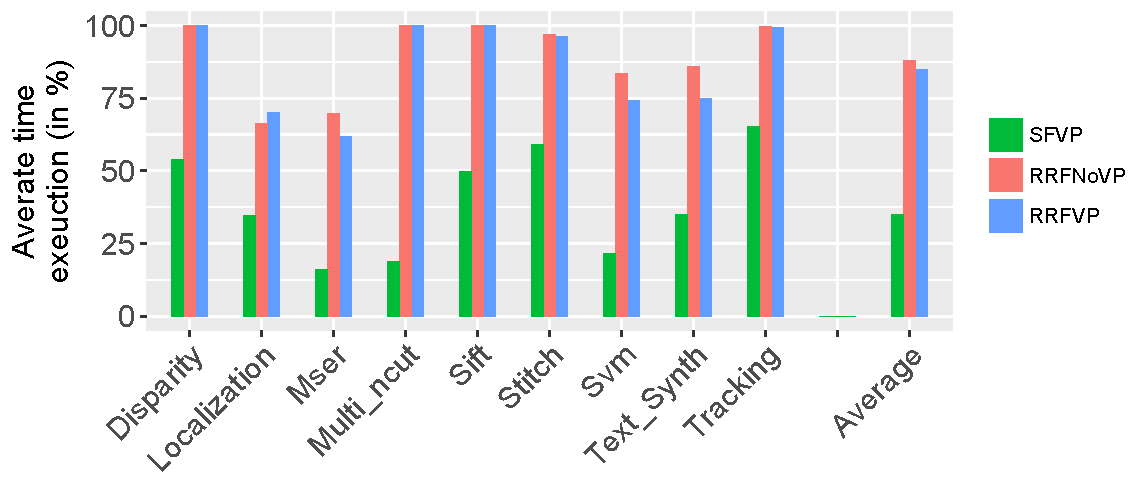
\includegraphics[width=1\textwidth]{chapter3/graphics/perf_av_cycle_exec4.pdf}
    \caption{Average time each core is executing blocks (in \%) for each benchmark, using the different configurations. Higher is better.}
    \label{fig:perf_av_cycle}
	\vspace{1em}
\end{figure}

\paragraph*{Active Cycles}
To better highlight how the SF scheme hinders performance even with value prediction, the percentage of time a core in a composition is actively executing code, for each benchmark, is shown in Figure~\ref{fig:perf_av_cycle}.
For each configuration, the number of cycles each core in a composition has instructions to execute is averaged out and then compared to the total execution time of the application.
When the average active time of a core is close to the total execution time, this means that the composition was efficiently used, as each core had a block to run throughout the program execution.

Figure~\ref{fig:perf_av_cycle} shows that \vp{} often has low active times when using a composition of 16 cores.
This is due to the fact that the SF scheme is slow, and thus, some cores are inactive, waiting to receive a fetch request from another core.
The lower the percentage is, the less likely there are going to be multiple blocks on different cores in flight which in turn means the composition is less efficient and value prediction is less useful.
Since value prediction is aimed at increasing instruction level parallelism (ILP)~\cite{peraisBeBop2015} it is important that cores may fetch blocks quickly in a composition.

%Of course, it is important to note that their LSQs and L1 caches may still be used by other active cores, simply that their execution units are not being used.


With the RRF scheme, the percentage of active time is increased on average by a factor of 2.28x, and is on average 85\%.
This means that during most of the execution of an application, all cores are executing code, and thus greatly increases the chance of improving performance via core composition.
It is interesting to see that \nfvp{} has a lower average time than \nfnovp{} for some benchmarks such as \bm{MSER} and \bm{Texture\_Synthesis}.
Also, whilst RRF aims to evenly distribute blocks amongst the cores, the average core utilisation for \bm{Localization} with the configurations \nfnovp{} and \nfvp{} is of 62\%.
This reduced average time is due to flushes caused by Load-Store-Queue (LSQ) violations, which causes cores to flush their instruction windows, and thus increases the number of times that cores will not be executing code.
Figure~\ref{fig:lsqvio} shows the number of blocks that cause an LSQ violation, normalised by the number of fetched blocks for each of the benchmarks.
Even though the percentage of violations is small, it still has an impact on how efficient the composition is, due to the fact that compositions rely on heavy speculation to obtain any performance improvements.
\begin{figure}[t]
    \centering
    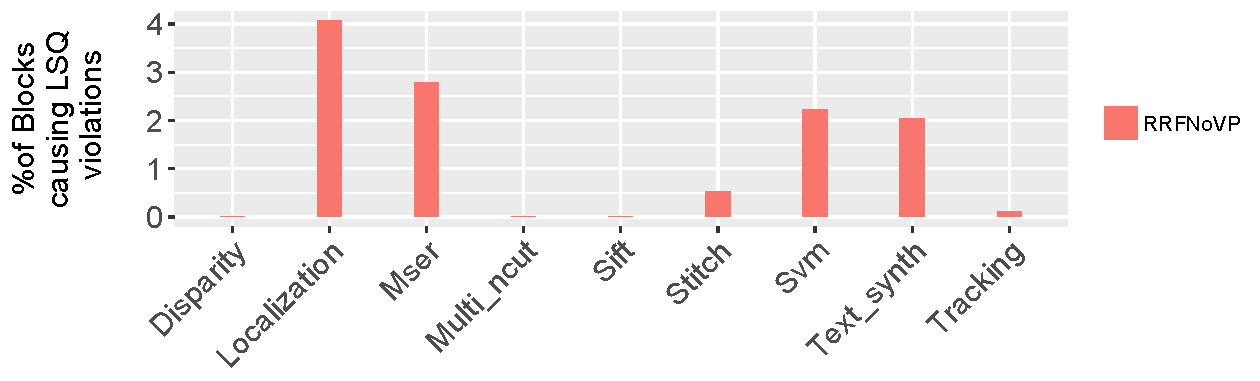
\includegraphics[width=1\textwidth]{chapter3/graphics/lsqViol4.pdf}
    \caption{Number of blocks that cause LSQ violations, normalised by the number of fetched blocks for each of the benchmarks.}
    \label{fig:lsqvio}
	\vspace{1em}
\end{figure}

%A store-set dependency predictor is implemented in the processor~\cite{chrysos1998storesets}, however it is sometimes hard to predict load-store dependencies across multiple blocks, which is why LSQ violations occur.
%Store-set dependency predictors are not discussed in more detail in this chapter, however researching how store-set dependencies could be applied to core-composition is an interesting subject for future work.

\subsection{Round robin fetching scheme bottleneck Analysis}

As seen in the previous section RRF enables better use of the perfect value predictor. 
However, on its own it often does not outperform \novp{}, averaging only a speedup of 1.05x.
This section covers where the bottlenecks of RRF are.%, what potential solutions can be employed, and how that can improve performance overall.

\paragraph*{Block dispatching latency}

RRF improves performance of a core composition by parallelising block fetches.
This is achieved through a round robin fetching scheme, where cores do not fetch blocks sequentially, but rather in strides.
Yet whilst blocks can be fetched out of order they must still be dispatched in order (recall Section~\ref{chp3:sec:fetch}).

\begin{figure}[t]
    \centering
    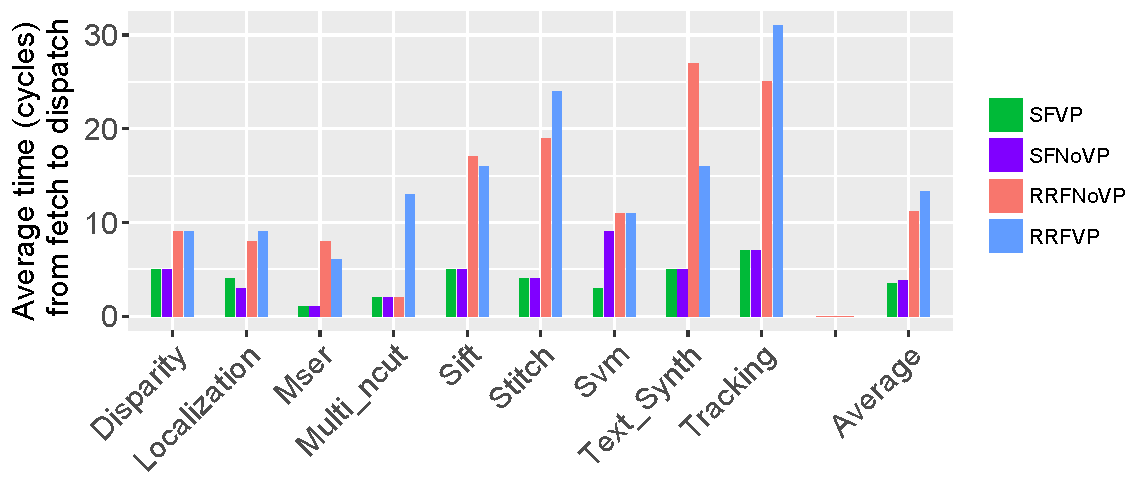
\includegraphics[width=1\textwidth]{chapter3/graphics/avTimeToFetch3.pdf}
    \caption{Average time (in cycles) for block to go from fetched to dispatched using the serial fetching scheme and round robin fetching scheme. Lower is better.}
    \label{fig:av_time}
	\vspace{1em}
\end{figure}

This means that cores may fetch blocks in their window that must wait a certain number of cycles before executing.
To understand how this affects the performance of the new fetching scheme, the average time from a block being fetched, to a block being dispatched is recorded in the simulator.
Comparing the average time between SF and RRF can provide an estimate as to how much performance is potentially lost.

Figure~\ref{fig:av_time} shows the average time for all the SD-VBS benchmarks using the different configurations.
As can be seen, for most benchmarks, RRF's average time is 2x slower than the current.
This is due to the fact that whenever the SF scheme fetches a block, it can immediately dispatched as fetches are serialised.
Surprisingly, \bm{Multi\_NCut} for \nfvp{} has a much longer time between fetching and dispatching a block.
This is due to the fact that \bm{Multi\_NCut} features blocks of only 11 instructions on average and with value prediction blocks are committing faster than on the other configurations.
%Given that a block must access a shared counter to check if it can dispatch, and the counter can only be incremented once per cycle (atomic increment), this shared resource is causing the long fetch to dispatch latency.
Given that only one block can be dispatched per cycle, this is causing the long fetch to dispatch latency.
Even with the extra latency, RRF still ensures that every core is full, cores must now only wait for their blocks to be dispatched, rather than having for a fetch request.

\begin{figure}[t]
    \centering
    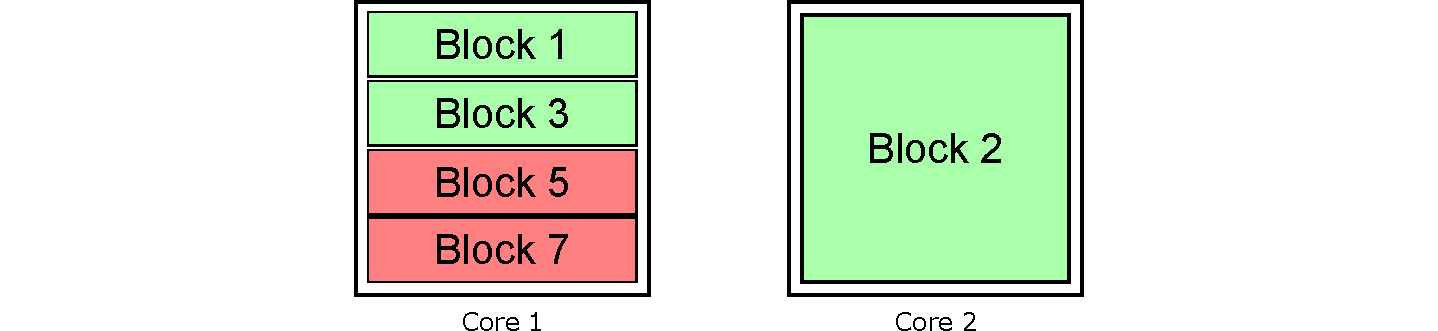
\includegraphics[width=1\textwidth]{chapter3/graphics/fetch_ex.pdf}
    \caption{Two core composition where cores fetch blocks of varying size. Green blocks represent blocks that can be dispatched, whilst the red blocks cannot.}
    \label{fig:var_ex}
    \centering
    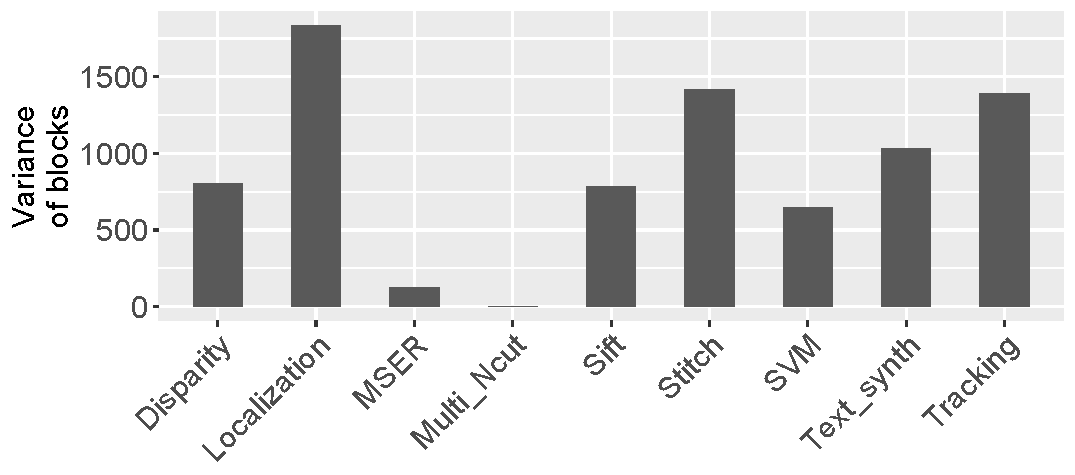
\includegraphics[width=1\textwidth]{chapter3/graphics/variance.pdf}
    \caption{Standard deviation of block sizes per benchmark.}
    \label{fig:variance}
	\vspace{1em}
\end{figure}
\paragraph*{Block size variance}
Another issue that can arise when fetching with a fixed stride is that if cores are fetching blocks of different sizes this may increase the fetch to dispatch latency.
For example, in the two core composition seen in Figure~\ref{fig:var_ex} the second core fetches Block 2 that is 128 instructions.
If Block 2 were smaller, Core 2 could fetch and dispatch blocks 4 and 6.
However, since Block 2 occupies the whole instruction window, Core 2 will have to wait for block 2 to commit before doing so.
Thus blocks 5 and 7 cannot be dispatched on Core 1 before block 2 has finished executing.

Figure~\ref{fig:variance} shows the variance of block sizes in the SD-VBS benchmarks.
This was obtained by counting the different block sizes each benchmark fetched, and grouping them into 4 distinct buckets: blocks that occupy 1, 2, 3 or 4 lanes in the window.
The Figure shows that the benchmark \bm{Multi\_NCut} features a very low variance; which is why RRF has a similar fetch to dispatch latency as SF without value prediction.

%The issue of variance is not only specific to RRF, as SF will also suffer from this issue as well.
%The difference is that with SF, Core 1 would not fetch blocks 3, 5 and 7, instead it would wait for Core 2 to commit its block and submit a fetch request.
%Of course, variance only partially provides an insight as to why core composition may be less efficient; as it does not take into account data dependencies between blocks.
%Also, the variance does not take into account that blocks of different sizes may belong to different phases.
%Nevertheless, it is an important factor to take into consideration.
%. Blocks are grouped up in buckets (occupy 1, 2, 3 or 4 segments).


%Explain how different blcok sizes may mess up the new fetching scheme

\subsubsection{Summary}

This section shows that a perfect branch predictor, paired with perfect value prediction and the round robin fetching scheme can outperform the current configuration by a factor of up to 3x and on average a speedup of 1.87x.%, and can potentially be improved to 2.35x with further modifications to the fetching scheme.
This section also showed that without value prediction RRF only obtains a 1.09x speedup compared to the serial fetching scheme.
This is due to the fact that the benchmarks all display a certain amount of data-dependencies between blocks and that spreading blocks across cores more evenly can put pressure on the NoC; thus reduce the performance improvements of fetching blocks quicker.

\label{chp:chp3:sec:analysis}
\section{Performance analysis using the block based D-VTAGE predictor}
This section evaluates a real implementation of a value predictor, using the block based D-VTAGE predictor.
Before conducting the performance analysis, it is important to understand how the predictor must be configured.
This section therefore starts with a block analysis of the SD-VBS benchmarks.

\subsection{Block analysis}
\begin{figure}[t]
    \centering
    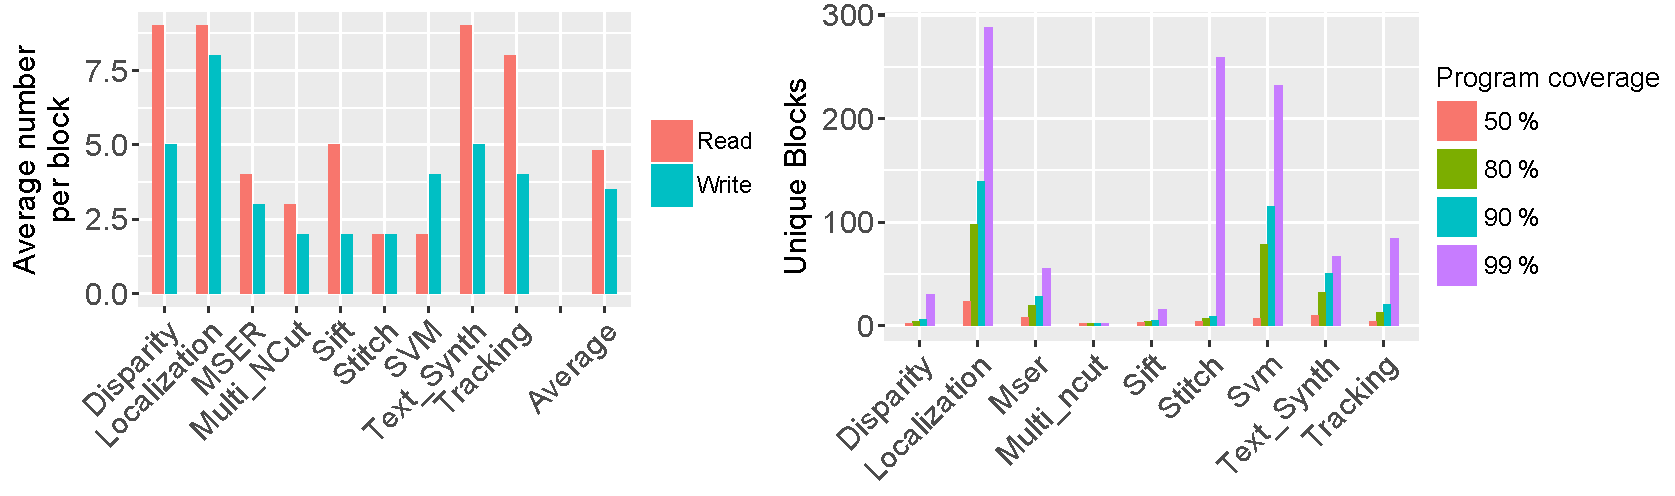
\includegraphics[width=1\textwidth]{chapter3/graphics/joint.pdf}

    \caption{Average number of register reads and writes per EDGE block and the number of unique blocks comprising different percentages of the total execution (in blocks) of each of the benchmarks.}
    \label{fig:edge_reg_read}
	\vspace{1em}
\end{figure}

In a block based D-VTAGE predictor a single prediction request fetches multiple values.
Due to the fact that the block size is fixed ahead of time~\cite{peraisBeBop2015}, determining the correct size is important.
Having a block with many values means that the D-VTAGE predictor can predict a higher amount of register reads in the EDGE block, however this comes at the expense of having less blocks in the predictor tables.
On the other hand, a small block size allows to have multiple blocks stored at a time but means that not all instructions can have their values predicted in the EDGE block.

In this chapter, the value predictor only predicts register reads.
This is due to the fact that register reads create data dependencies amongst blocks, as discussed in Section~\ref{chp3:sec:val}.
Focusing only on register reads also reduces the the block size requirements as there is often only a few reads in an EDGE block.
To determine the size, all the EDGE blocks of the SD-VBS benchmarks are anaylsed to determine the average register read and write count is per block.
The writes are tracked as it provides information on the potential amount of register dependencies found in each of the applications.

The left hand side of figure~\ref{fig:edge_reg_read} shows the average number of register read and writes for each of the benchmarks.
On average, there are 5 register reads and 3 register writes per block.
Whilst \bm{Disparity} \bm{Localization}, \bm{Texture\_Synthesis} and \bm{Tracking} have higher register read counts than the average, most of them only have 5 writes per block.
This means that having a D-VTAGE block size of 5 could capture all dependencies; however this would require some detection of which reads are data-dependent, which is beyond the scope of this thesis.
Since Section~\ref{chp:chp3:sec:analysis} showed these benchmarks benefit from value prediction, to ensure that most blocks have all their register reads captured, a block size of at least 8 is required.

\paragraph*{Block variation analysis}

%\begin{figure}[t]
%    \centering
%    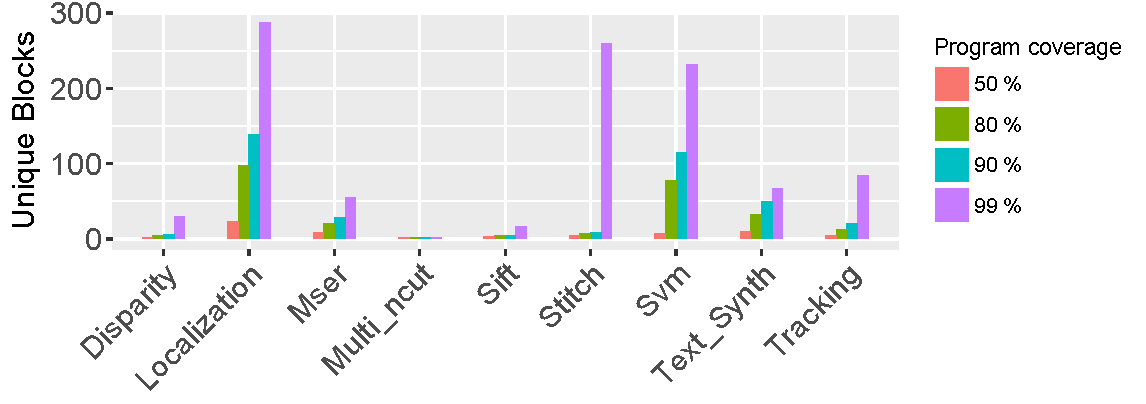
\includegraphics[width=1\textwidth]{chapter3/graphics/unique_blocks.pdf}%

%    \caption{Number of unique blocks comprising different percentages of the total execution (in blocks) of each of the benchmarks.}
%    \label{fig:totblock}
%	\vspace{1em}
%\end{figure}

One method of understanding how the block based D-VTAGE predictor will perform is to study the number of unique blocks found in each of the benchmarks.
Benchmarks that feature a smaller number of unique blocks can potentially benefit more from value prediction as the predictor cannot hold many blocks at a time.
Reporting all unique blocks executed is not a proper evaluation of the variety of blocks found in the benchmark, as some will most certainly be executed more times than other.
To account for this, blocks are sorted by number of occurrences in descending order, and then added to the unique block counter as long the number of occurrences of visited blocks is under a percentage of total number of blocks executed.

The right hand side of figure~\ref{fig:edge_reg_read} shows the number of unique blocks found in each benchmark that account for 50,80,90 and 99\% of the total number of executed blocks.
As can be seen, applications \bm{Disparity}, \bm{Multi\_NCut} and \bm{Sift} \bm{Stitch} and \bm{Tracking} execute less than 50 unique blocks during 90\% of its total execution.
This is promising as it means that there is a high chance that the predictor requires less entries to capture all possible blocks in the application.
On the other hand, \bm{Localization}, and \bm{SVM} execute over 100 blocks throughout 90\% of their execution, twice as many as the previously mentioned benchmarks.
For these applications, it might be harder to predict values as new blocks may overwrite entries in the predictor.


\subsection{Setup}

\begin{table}[t]
\small
\centering
\begin{tabular}{p{5.2cm} p{3cm}}
\toprule
\textbf{Parameter} & \textbf{Values} \\ \midrule
\# Base Entry & 1536\\
\# Tagged & $6\times1536$\\
\# Block in Spec Window & 4 \\ \hline \midrule
\# of values per entry & 8, 16\\
Confidence Value & 4 or 7 with FPC \\ \bottomrule
\end{tabular}
  \caption{D-VTAGE table configuration and configurable parameters.}\label{tab:vtage-conf}
\vspace{1em}
\end{table}

This section demonstrates how the block based D-VTAGE value predictor improves the performance of core composition using the round-robin fetch scheme (RRF).
Serial fetch is not explored since previous section showed that when using value prediction, RRF always provides the best results.
The results reported in this section represent the culmination of hardware modifications for core composition discussed in this chapter.
All benchmarks are executed using a 16 core composition.

\paragraph*{Predictor size}
The D-VTAGE size configuration can be found in Table~\ref{tab:vtage-conf}.
The Last-Value Table shares the same number of values as the Base Entry and uses a 5-bit tag.
Each tagged entry has a tag of varying size (first table is 12 bits, second 13 bits so on and so forth).
The total number of values for the D-VTAGE predictor is taken from Perais et al's work ~\cite{peraisBeBop2015}.
The adopted size for this chapter is the medium predictor as it provides a good compromise between performance and total size of the predictor.
The blocks in the speculative window represents the total number of in-flight blocks that can be handled by the speculative window, which is 4.

\paragraph*{Parameter tuning}
Two features of the predictor can be modified: the number of values per entry and at what confidence a prediction is used.
Modifying the required confidence explores the trade-off between high coverage and low misprediction.
The original D-VTAGE uses Forward Probabilistic Counters (FPC)~\cite{riley2006fpc} to increment the confidence, and only used predictions once the counter was set to 7.
This confidence rate ensured that the predictor had an accuracy of over 99\%, but at the expense of a low coverage, 20\% on average~\cite{peraisBeBop2015}.
The confidence of 4 is chosen as it allows for very fast deployment of predictions, whilst still ensuring that the values have been trained at least a few times.
The FPC vector used in this Chapter is the same as the one in Perais et al.'s work $\{1,\frac{1}{16},\frac{1}{16},\frac{1}{16},\frac{1}{16},\frac{1}{16},\frac{1}{32},\frac{1}{32}\}$.
 

%This section explores two counter scenarios: using a prediction when the confidence is set to 4 (without FPC), and using confidence when the counter is set to 7 (with FPC).
%To briefly summarise FPC: when a value is correctly predicted, its confidence is incremented based on a probability, rather than always incrementing the counter by one.

%\begin{table}[t]
%%  \small
 % \centering
% \begin{tabular} {| l | l | l |}
% \hline%
%	\#Base Entry. & \#Tagged & \#Block in Spec Window\\ \hline
%	1536 & $6\times1536$ & 4 \\ \hline
%	\end{tabular}
 % \caption{D-VTAGE table configuration.}\label{tab:vtage-conf}
%\end{table}

%\begin{table}[t]
%\small
%\centering
%\begin{tabular}{p{5.2cm} p{1.8cm}}
%\toprule
%\textbf{Parameter} & \textbf{Values} \\ \midrule
%\# of values per entry & 8, 16\\
%Confidence Value & 4 or 7 with FPC \\ \bottomrule
%\end{tabular}
%\caption{Configurable parameters for D-VTAGE}\label{tab:vtage-params}
%\end{table}
\paragraph*{Block size}
Table~\ref{tab:vtage-conf} also shows the possible values that can be taken for the two parameters.
Whilst this section showed that most applications only have 5 reads per block,  \bm{Disparity} and \bm{Localization} have at least 8 reads and they both benefit from value prediction as seen in Section~\ref{chp:chp3:sec:analysis}.
Since there is currently no method of determining which reads may have data-dependencies, it is important to have a block size that captures the largest register read average for the set of benchmarks which is 8.
This section explores block sizes of 8 and 16 to ensure that all register reads are potentially covered. 
The block size of 16 is explored to see how capturing a higher number than the average number of reads affects the performance of the predictor. 

\paragraph*{Prediction Delay}
In the original D-VTAGE proposal, they suggest that the predictor can generate \textit{x} values per cycle where \textit{x} is the issue width of the core.
This means that 4 values can be generated per cycle, as this is the issue width of a core (see Chapter~\ref{chp:setup} Section~\ref{chp:setup:conf}.
In Section~\ref{chp:chp3:sec:analysis}, Figure~\ref{fig:av_time} showed that, when using RRF, the minimum cycles from fetch to dispatch was 10, meaning that the predictor can issue 8 to 16 predictions before dispatching any block.


\subsection{Results}

\paragraph*{Performance}

\begin{figure}[t]
    \centering
    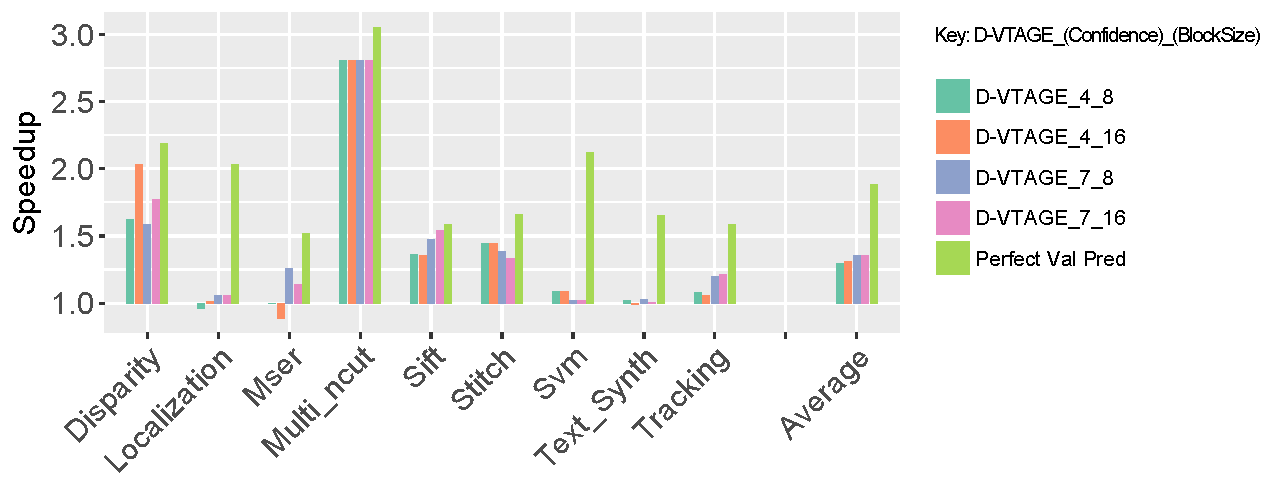
\includegraphics[width=1\textwidth]{chapter3/graphics/vtage_speed3.pdf}
    \caption{Speedup obtained using a D-VTAGE value predictor and RRF with 16 cores composed. Baseline is 16 cores composed with SF and without value prediction. Both use perfect branch prediction. Higher is better.}
    \label{fig:vtage_perf}
	\vspace{1em}
\end{figure}

Figure~\ref{fig:vtage_perf} reports the speedup obtained with the different configurations of the D-VTAGE predictor with RRF.
The baseline is a 16 core composition that uses the serial fetching (SF) scheme without any value prediction and using perfect branch prediction.
The lack of value prediction and use of serial fetching represents the current implementation of core composition.
To better understand the performance of the predictors, each configuration is compared to the perfect predictor, which can predict every register value at any instance.
Throughout this section, the configurations of D-VTAGE are labeled: \textbf{D-VTAGE\_\textit{Confidence}\_\textit{BlockSize}}.

On average, using a D-VTAGE value predictor with the RRF scheme results in an average speedup of 1.32x.
When comparing the performance between the different configurations, the main observation is that using a higher confidence results in better performance, however slight, 1.35x for D-VTAGE\_7\_16 compared to 1.31x for D-VTAGE\_4\_16.
However, for the benchmark \bm{Disparity} using a higher confidence leads to less of a performance increase 1.75x speedup compared to 2.0x for a confidence counter of 4.
This is due to the fact that \bm{Disparity} is composed of loops with highly predictable values, and thus deploying predictions faster results in better performance improvements without risking a higher misprediction rate.
On the other hand, \bm{Localization} and \bm{MSER} performs worse with a lower confidence counter, and result in a slowdown.
Benchmarks \bm{Sift} and \bm{Tracking} perform better with a higher confidence, but the results of using a 4 bit counter never negatively impact performance.

The 16 values per block does not lead to better performance than 8 values but stays on par with it.
The only noticeable difference is with \bm{MSER} where the smaller block performs better.
A lower number of values per block allows the predictor to capture a higher variety of executed blocks.
Figure~\ref{fig:edge_reg_read} shows that \bm{MSER} has at least 50 different blocks throughout 99\% of its execution, and on average, only 3 register reads per block.
Therefore, for \bm{MSER}, a predictor with less values per entry can capture more of the variation.
On the other hand, for \bm{Disparity}, 16 values per entry is required to get the best performance.
This once again corroborates with the information from Figure~\ref{fig:edge_reg_read}.
\bm{Disparity} has a higher average of reads per block, but features a very low number of unique blocks.
Therefore having a larger entry in the table captures more values, but does not suffer from having entries being replaced by new blocks.

Comparing the performance of the different configurations to the perfect value predictor, it is apparent that most benchmarks do not achieve their maximum potential as the perfect predictor results in an average speedup of 1.88x compared to 1.32x of D-VTAGE.
However, benchmarks \bm{Disparity} and \bm{Multi\_NCut} show how value prediction with RRF is a promising lead for improving the performance of core composition.

\paragraph*{Coverage and Accuracy}
To better understand the performance of the different D-VTAGE configurations, the predictors' coverage and misprediction rates are recorded.
The coverage is measured by comparing the number of correct register read values to the total number of executed register reads.
Since EDGE is a block based architecture, it is important to study the coverage and accuracy on both a per-instruction level and per-block level.
This is due to the fact that a single read misprediction leads to flushing the block and all younger blocks in the chain.
Thus whilst the misprediction rate for predicted instructions may be low, it can have a large impact as up to 64 blocks may be in flight, and may all need to be flushed.
Also a single accurate register prediction may not necessarily improve performance as other un-predicted registers in the block may be data-dependent with other blocks, reducing ILP.

\begin{figure}[t]
    \centering
    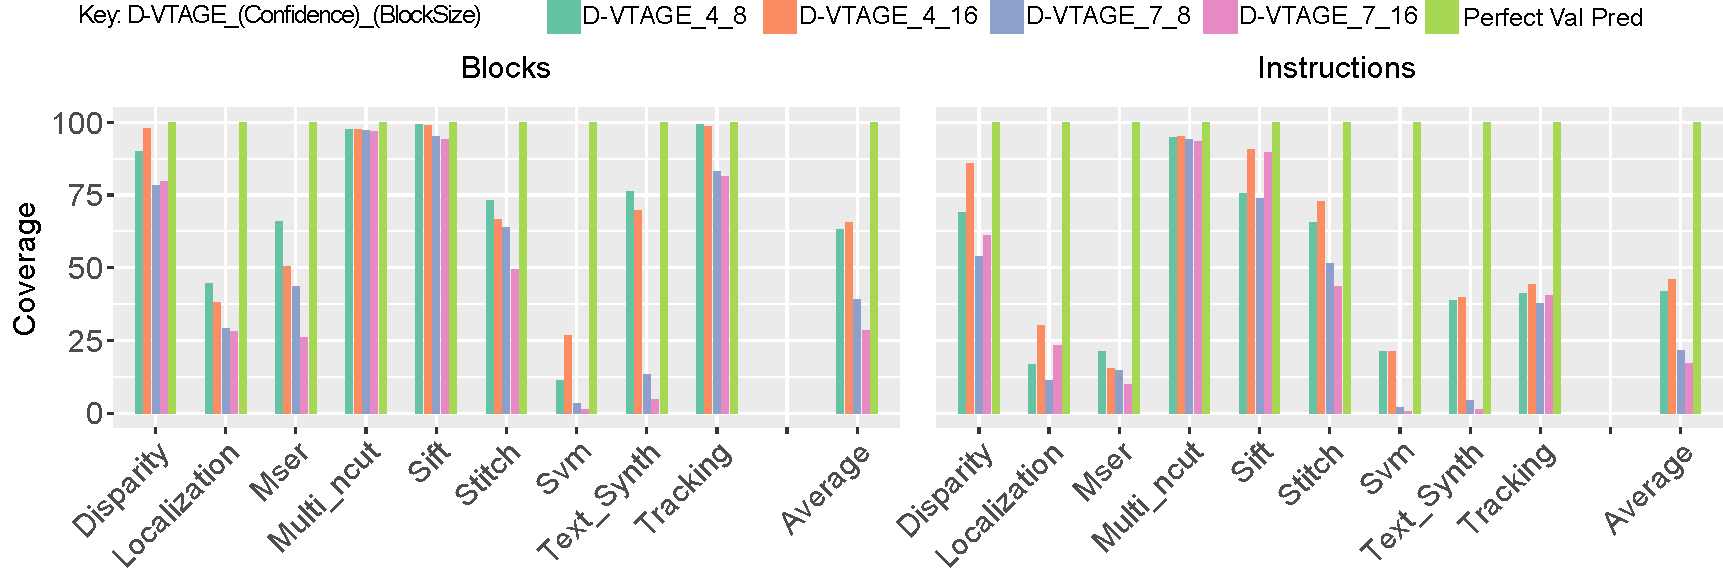
\includegraphics[width=1\textwidth]{chapter3/graphics/coverageFull2.pdf}
    \caption{Prediction coverage at a block and instruction level. Higher is better}
    \label{fig:vtag_cov_block}
	\vspace{1em}
\end{figure}

In this chapter, only blocks that are committed count towards the predicted blocks as any flush will artificially inflate the coverage count.
Figure~\ref{fig:vtag_cov_block} displays the number of blocks which have at least one prediction, relative to the total number of committed blocks and the number of predicted register reads relative to the total executed register reads.
The figure shows similar patterns for both coverages: the predictors with lower confidence counters have a higher coverage, 65\% compared to 31\% for the high confidence counter.
This is normal: lower confidence allowes predictions to be used with faster, which will increase coverage.

Whilst the block coverage is high, the coverage for registers reveals that not all registers are being predicted.
Once again, lower confidence equates to higher coverage, however this time it's 30\% for a confidence of 4 and under 25\% for a confidence of 7.
The register coverage for a confidence of 7 is in line with the coverage reported in Perais. et al's work ~\cite{peraisBeBop2015, peraisVTAGE2014} if not slightly higher.
The coverage may be slightly higher due to the fact that the values being predicted are often either loop increments or memory increments which can easily be predicted.

The register coverage helps explain why the high block coverage does not lead to better performance: whilst most blocks may have a valid prediction, some of the register reads cannot be predicted.
This may be due to data being carried over which is unpredictable; for instance a loop which sums all values of an array into a single integer will pass that integer via a register.
This register will cause a data dependency between loop iterations and will be difficult to predict.

\begin{figure}[t]
    \centering
    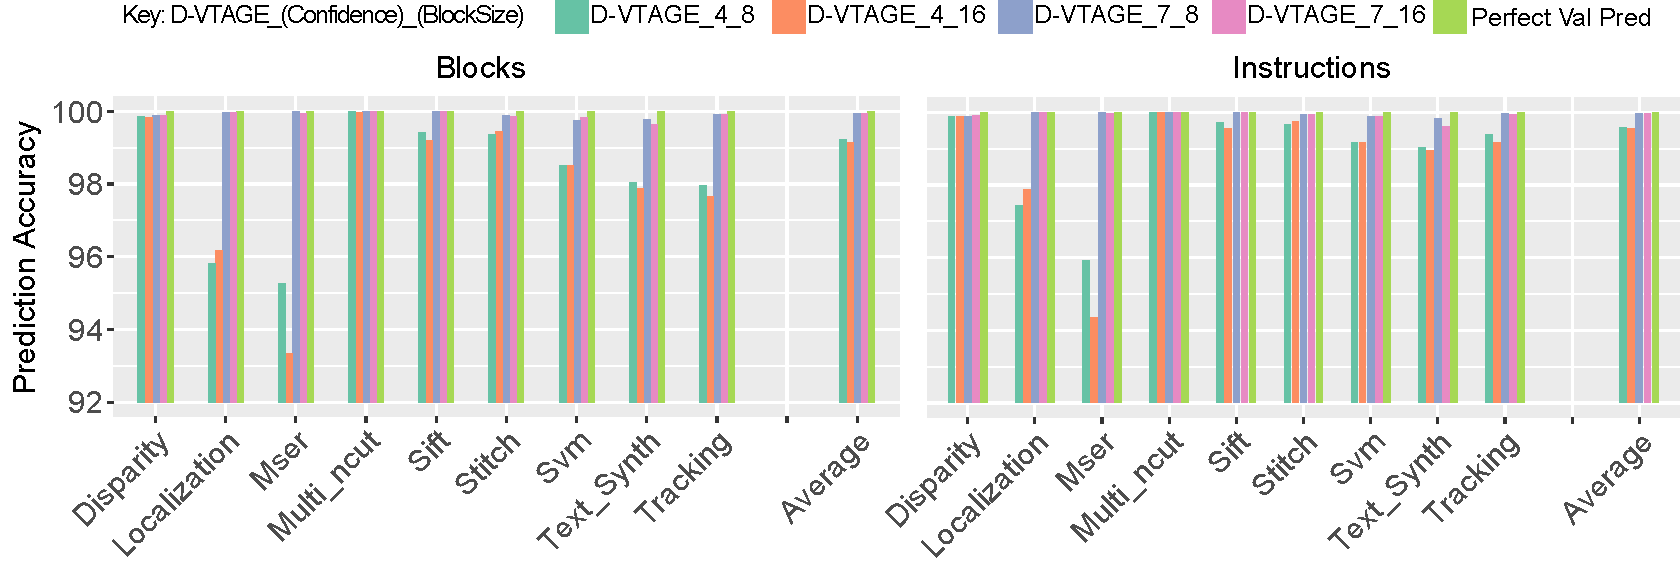
\includegraphics[width=1\textwidth]{chapter3/graphics/predAcc2.pdf}
    \caption{Accuracy of the different D-VTAGE predictors at a block and instruction level. Higher is better.}
    \label{fig:vtag_accuracy_block}
	\vspace{1em}
\end{figure}

\bm{Localization}, \bm{MSER}, \bm{SVM} and \bm{Texture\_Synthesis} often have much lower coverage than the rest of the programs.
Recalling Figure~\ref{fig:edge_reg_read} which shows the number of unique blocks executed throughout the programs, these benchmarks had a higher count of unique blocks.
This explains why the coverage will be lower: there's a higher chance of encountering a new block than executing a known one.
As blocks require multiple executions to train the predictor (if the values in the register are indeed predictable), than the higher diversity of blocks makes it harder.
Thus, these benchmarks will naturally have a harder time to benefit from value prediction.

Figure~\ref{fig:vtag_cov_block} shows that a lower confidence allows for higher coverage, yet the speedups seen in Figure~\ref{fig:vtage_perf} indicate that a higher confidence leads to better performance.
To confirm this, Figure~\ref{fig:vtag_accuracy_block} presents the prediction accuracy rate for each benchmark at a per-block and per-instruction base respectively.
The D-VTAGE predictor maintains a 99\% accuracy, whether at the block level or instruction level.
However, for \bm{Localization}, \bm{MSER}, \bm{SVM}, \bm{Texture\_Synthesis} and \bm{Tracking}, the block level accuracy for a confidence of 4 is under 98\%, and even down to 93\% for \bm{MSER}.
The effect of a value misprediction is similar to a branch misprediction: it causes a flush of all blocks younger than the block with the incorrect misprediction.
Just like branch prediction, large core compositions are very sensitive to mispredictions, thus an accuracy rate of 93\% will impact performance if the blocks are small.
This explains why the low confidence counter sometimes performs worse than the higher confidence as it mispredicts more often.

\subsection{Performance with non-perfect branch prediction}

\begin{table}[t]
  \small
  \centering
 \begin{tabular} { | l | l | l | l | l | }
 \hline
   \cellcolor[gray]{0.7}Disparity & \cellcolor[gray]{0.7} Localization& \cellcolor[gray]{0.7} MSER& \cellcolor[gray]{0.7} Multi\_NCut& \cellcolor[gray]{0.7} Sift\\ \hline
	98\%  & 95\% & 85\%  & 100\%& 99\%\\ \hline
	 \cellcolor[gray]{0.7} Stitch & \cellcolor[gray]{0.7} SVM & \cellcolor[gray]{0.7} Text. Synth & \cellcolor[gray]{0.7} Tracking&\\ \hline
	  95\%& 93\%& 98\%& 98 \%&\\ \hline
	\end{tabular}
  \caption{Branch prediction accuracy in percentage for each of the benchmarks.}\label{tab:sd-vbsbpred2}
  \vspace{-1em}
\end{table}

\begin{figure}[t]
    \centering
    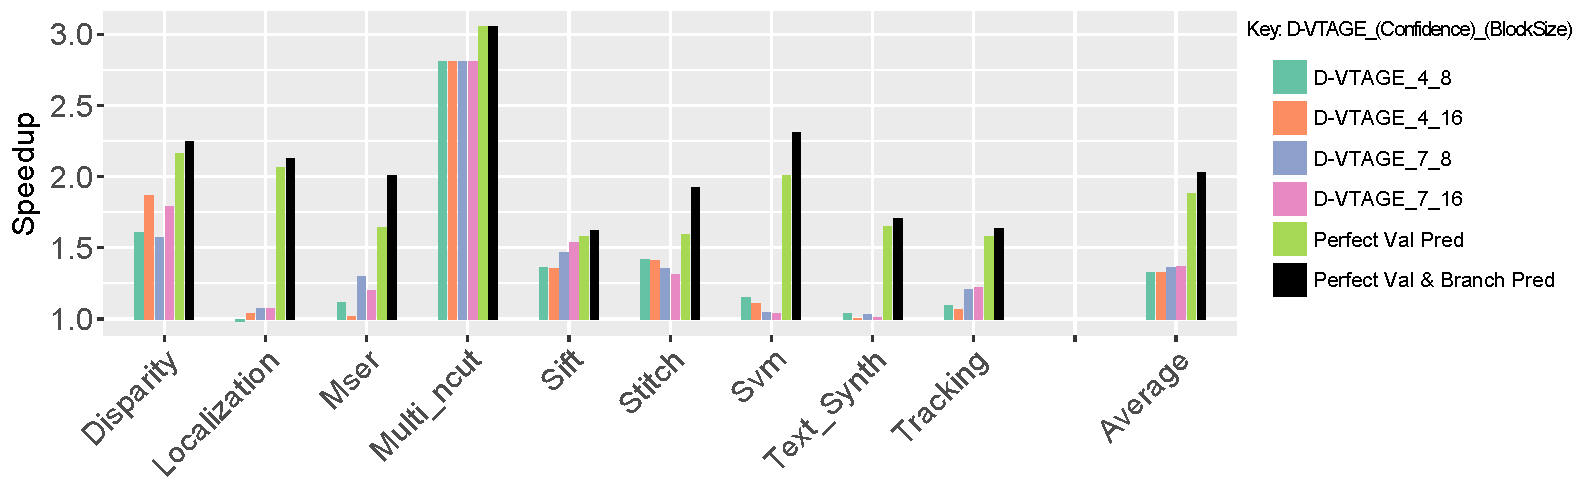
\includegraphics[width=1\textwidth]{chapter3/graphics/with_bpred.pdf}

    \caption{Speedup obtained using a D-VTAGE value predictor and RRF with 16 cores composed. Baseline is 16 cores composed with SF and without value prediction. Both use a non-perfect branch predictor. Higher is better.}
	\vspace{1em}
    \label{fig:bpred}
\end{figure}
Finally, this section studies how non-perfect branch prediction affects the performance of the applications with RRF and value prediction.
To conduct this analysis, the perfect branch predictor was modified to randomly mis-predict given a certain accuracy requirement.
For each of the benchmarks, the branch prediction accuracies recorded in Chapter~\ref{chp:cases} are used.
These accuracies can be found in Table~\ref{tab:sd-vbsbpred2}.

Figure~\ref{fig:bpred} reports the speedup obtained with the different configurations using a non-perfect branch predictor.
In this scenario, the baseline is a 16 core composition with SF and no value prediction, using the branch prediction accuracies defined in Table~\ref{tab:sd-vbsbpred2}.
The figure shows an extra configuration that shows the results of the perfect value prediction with perfect branch prediction, to give perspective of how branch prediction affects performance.
As the figure shows, the new configuration still performs well, due to the fact that most benchmarks had either high enough branch prediction accuracies, or blocks large enough to sustain 16 composed cores.
This confirms that even without perfect branch and value prediction, performance can be improved by up to 2.8x, with an average of 1.30x.



%\subsubsection{Size of stride}

%\begin{figure}[t]
%    \centering
%    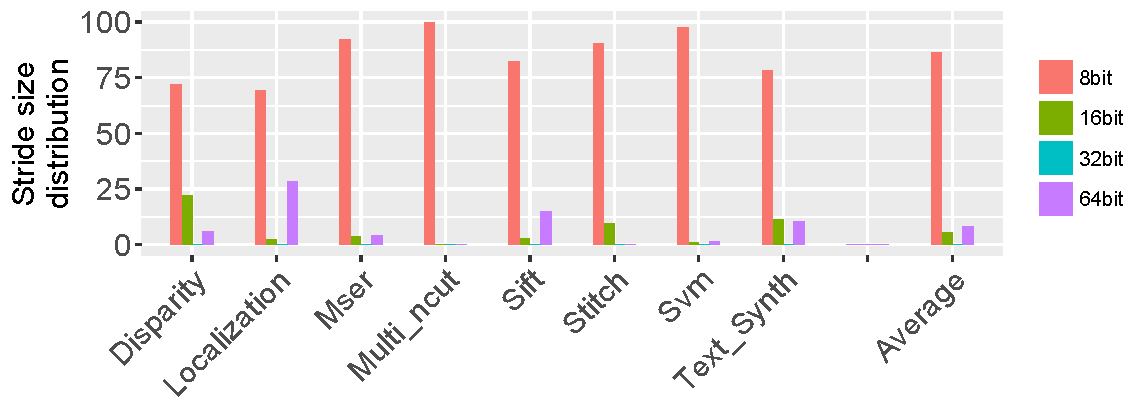
\includegraphics[width=1\textwidth]{chapter3/graphics/strides.pdf}
%    \caption{Distribution of the size of strides for each benchmark.}
%    \label{fig:strides}%
%	\vspace{1em}
%\end{figure}

%Whilst 64 bit strides are used throughout the experiments to capture all the potential performance, 64 bits per entries may not be necessary.
%Figure~\ref{fig:strides} shows the average number of valid predictions whose strides could fit in either an 8, 16, 32 or 64 bit signed integer for each of the benchmarks.
%The data was taken from the D-VTAGE configuration that led to the highest performance overall for each of the benchmarks.
%In Perais' et al'.s work they recommend that a medium-sized D-VTAGE predictor use 8-bit strides.
%Overall, Figure~\ref{fig:strides} shows that using 8 bit strides should be sufficient for most benchmarks, however \bm{Disparity}, one of the benchmarks which benefits most from value prediction, would lose almost 25\% of its coverage.
%Therefore, for these set of applications, a stride of at least 16 bits is necessary, as it captures 91\% of the total strides found in all the benchmarks.

%\subsection{Putting it all together}
%This section has demonstrated that a real value predictor can sometimes perform as well as a perfect predictor, resulting in a speedup of up to 2.7x for \bm{MSER} and 2x \bm{Disparity}, when paired with the round robin fetching scheme.
%The section also showed that whilst a lower confidence rate does increase the coverage, it does lead to a higher misprediction.
%As core composition is sensitive to any kind of misprediction that causes a flush, the predictor with confidence value 4 performs less well than confidence value 7 with FPC.
%Finally, the analysis of stride size shows that for this set of benchmarks, a 16 bit stride is sufficient to capture 91\% of the strides for the benchmarks.
%Using this information, a recommended D-VTAGE configuration for the dynamic multicore processor would take up 39kB of memory, which is slightly larger than an L1 cache.
\label{chp:chp3:sec:analysis2}
\section{Conclusion}
This chapter has investigated how the current hardware used for core composition can be modified in order to improve performance.
Due to the fact that blocks are fetched in a serial fashion, when a large number of cores is composed this can severely reduce the amount of time that all cores are actively executing blocks.
Therefore, finding a way of allowing cores to fetch in parallel can help increase the effectiveness of a composition.
However, another issue arises, inter-block communication via register reads and writes can cause potential data-dependencies, which serialises the execution of blocks.
As register files are shared between cores when they are composed, cores may have to send read requests to cores that are physically far away, increasing the latency of read instructions.
Finding a way to predict data can potentially aleviate data dependencies and reduce the effect of high latency reads, thus further improve the performance of core composition.

This chapter proposed a round-robin fetching mechanism, where cores do not fetch sequential blocks, but rather fetch blocks in strides.
This enables cores to fetch independently from one another, without having to submit fetch requests to other cores.
Using such a scheme can potentially increase the performance of large core compositions on small blocks by a factor of 2 to 3x.

After covering the fetching scheme, the idea of using a block-based value predictor was covered.
This value predictor was initially designed by Perais. et al. in ~\cite{peraisVTAGE2014, peraisBeBop2015}.
The design choices behind the value predictor match some of the architectural features of EDGE, mainly to do predictions at the granularity of a block.

To understand how these two modification can impact performance, the same set of benchmarks used in Chapter~\ref{chp:cases} are explored here.
First, the performance of a perfect value predictor with the round robin fetching scheme is explored and shows that it can improve the performance of core composition by up to 3x, with an average of 1.88x.
The analysis demonstrated that without value prediction, the new round robin fetching scheme cannot improve performance on its own, due to the higher stress on the NoC and data-dependencies not resolving quickly enough.
This was followed by an analysis of the performance of using different configurations of the D-VTAGE value predictor.
Overall, using state-of-the art value prediction with round-robin fetching scheme leads to a performance improvement of up to 2.7x with an average of 1.3x.
To summarise, the main contributions of the chapter are:

\begin{itemize}
\item The proposal of a round robin fetching scheme where cores fetch in parallel, out of order, and dispatch in order, allowing for an average improvement of 50\% over the serial fetching scheme when considering value prediction.
\item Demonstration that by only predicting register read instructions, the performance of compositions can be improved by up to 1.5x with serial fetching and 3x with round robin as it alleviates data dependencies between blocks and reduces the impact of the network on chip.
\item An exploration of different configurations for a block based D-VTAGE value predictor with the new round robin fetching scheme, resulting in an average 1.33x speedup compared to the current composition mechanism, and up to a 2.7x performance increase.
\end{itemize}

This Chapter demonstrates that there is potential for more hardware support to make dynamic multicore processors more practical.

%% !TEX TS-program = pdflatex
% !TEX encoding = UTF-8 Unicode

% This is a simple template for a LaTeX document using the "article" class.
% See "book", "report", "letter" for other types of document.

\title{Understanding fetching performance on a core-fusion enabled processor}

\section{Setup}
In this section we will use a 16 core EDGE CPU and vary the number of segment lanes it can have.
Lanes define the number of blocks that can be in flight in parallel on a single core.
As an EDGE block can be a maximum of 128 instructions, each lane in a core will only be able to fetch a block which is 128/number of lanes large.
In the rest of the report I will use $E\textit{i}_n$ where i is the number of fused cores and n is the number of segments.

Throughout the rest of the report we assume a perfect L1 cache, so a block can be fetched in 1 or 2 cycles.

In this report we will see how having more lanes is, at least for a single core, advantageous due to the average size of a block.
However, as we will discover, this increases the overhead when it comes to core fusion, at least in its current form.

\section{Fetching overhead}
\subsection{On a single core}

The fetching procedure in a single core, $E1_4$ the fetching procedure behaves like this:

In a $E1_4$, as long as the core has a block in flight, it will attempt to fetch a new block every cycle.
A new block can be fetched as long as the header of the previous block has been decoded, which helps mask the latency of fetching a block from Icache.
With this information in hand, the fetch steps can be described as following:
\begin{itemize}
\item Cycle 1: Fetch block header
\item Cycle 2: Decode block header
\item Cycle 3: Make branch prediction
\item Cycle 4: Fetch new header.
\end{itemize}
A single core therefore requires, at minimum, about 10 cycles to fetch 4 block headers.

\subsection{On a core-composition}

When fusing cores, the current model used is defined as followed: Core $C_n$ will fetch blocks until it has filled all its segments; once this has been satisfied, it sends a prediction to $C_{n+1}$.
If $C_{n+1}$ currently has no blocks it will simply wait until it is sent a prediction.

To illustrate how this can become a problem I have profiled the twolf\_1 microbenchmark described here bellow:
\begin{lstlisting}
for (i = 0; i < loopcount; i ++)
{
    delta_cost = 10 - i * 100 /loopcount;
    fred =  ((double) delta_cost * cost_scale_factor ) / T ; 
    if( fred >= 0.0 ) 
        truth = 1 ;
    else if( fred < -80.0 )  
        truth = 0 ;
    else if( fred > -0.0001 ) 
    {
        if( 1.0 + fred > ( (double) RAND / (double)0x7fffffff ) )  
            truth = 1 ;
        else 
	 truth = 0 ;
    }
   else 
   {
         fract = (int)( -fred * 8388608.0 ) ;

          if((table1[ (fract >> 20) & MASK ] * 
              table2[ (fract >> 10) & MASK] * 
              table3[ fract & MASK ]) > 
              ( (double) RAND / (double)0x7fffffff ) ) 

                  truth = 1 ;
         else 
            truth = 0 ;
    }
}
\end{lstlisting}

The reason I chose this benchmark is due to the small blocks it will generate.

\begin{figure}
\center
  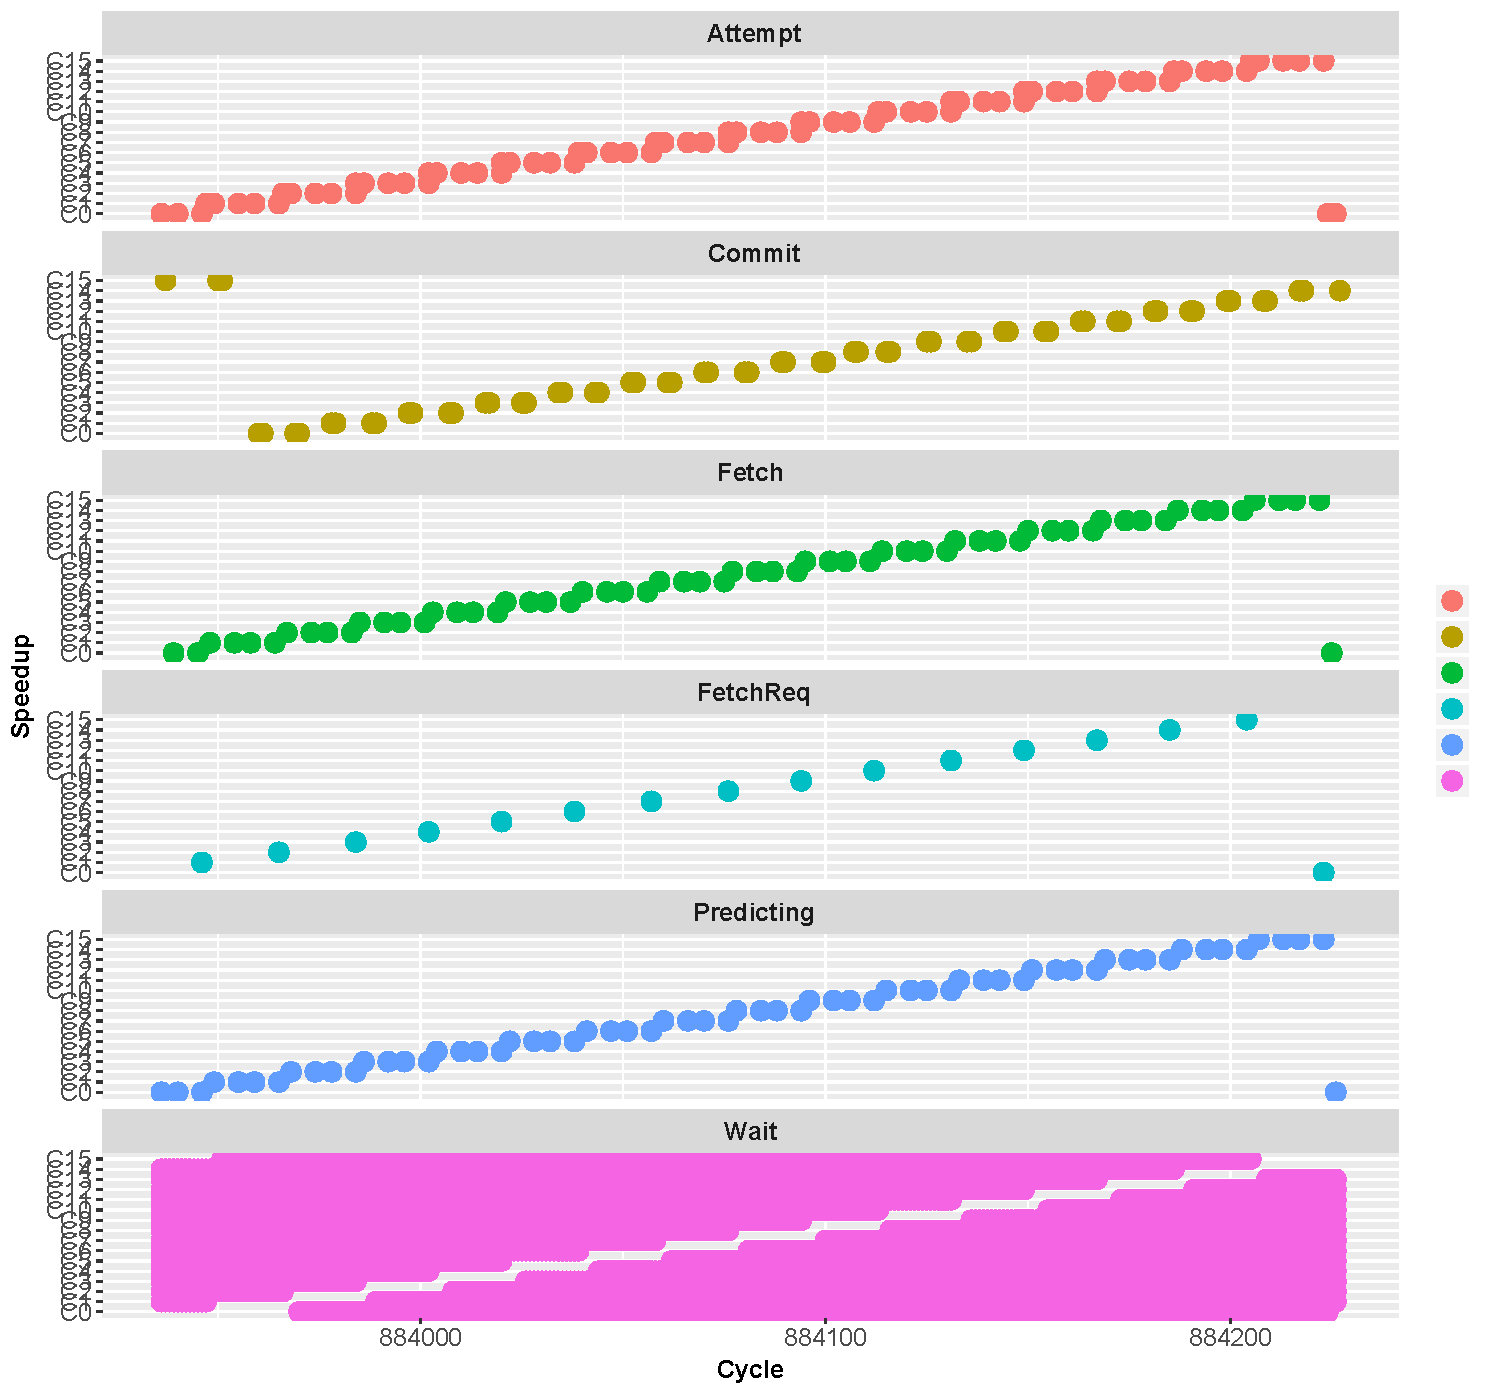
\includegraphics[width=1\textwidth]{chapter3/graphics/twolf_16.pdf}
  \caption{TWOLF on 16 cores fused, 4 segments each}\label{fig:16step}
\end{figure}

\begin{figure}
\center
  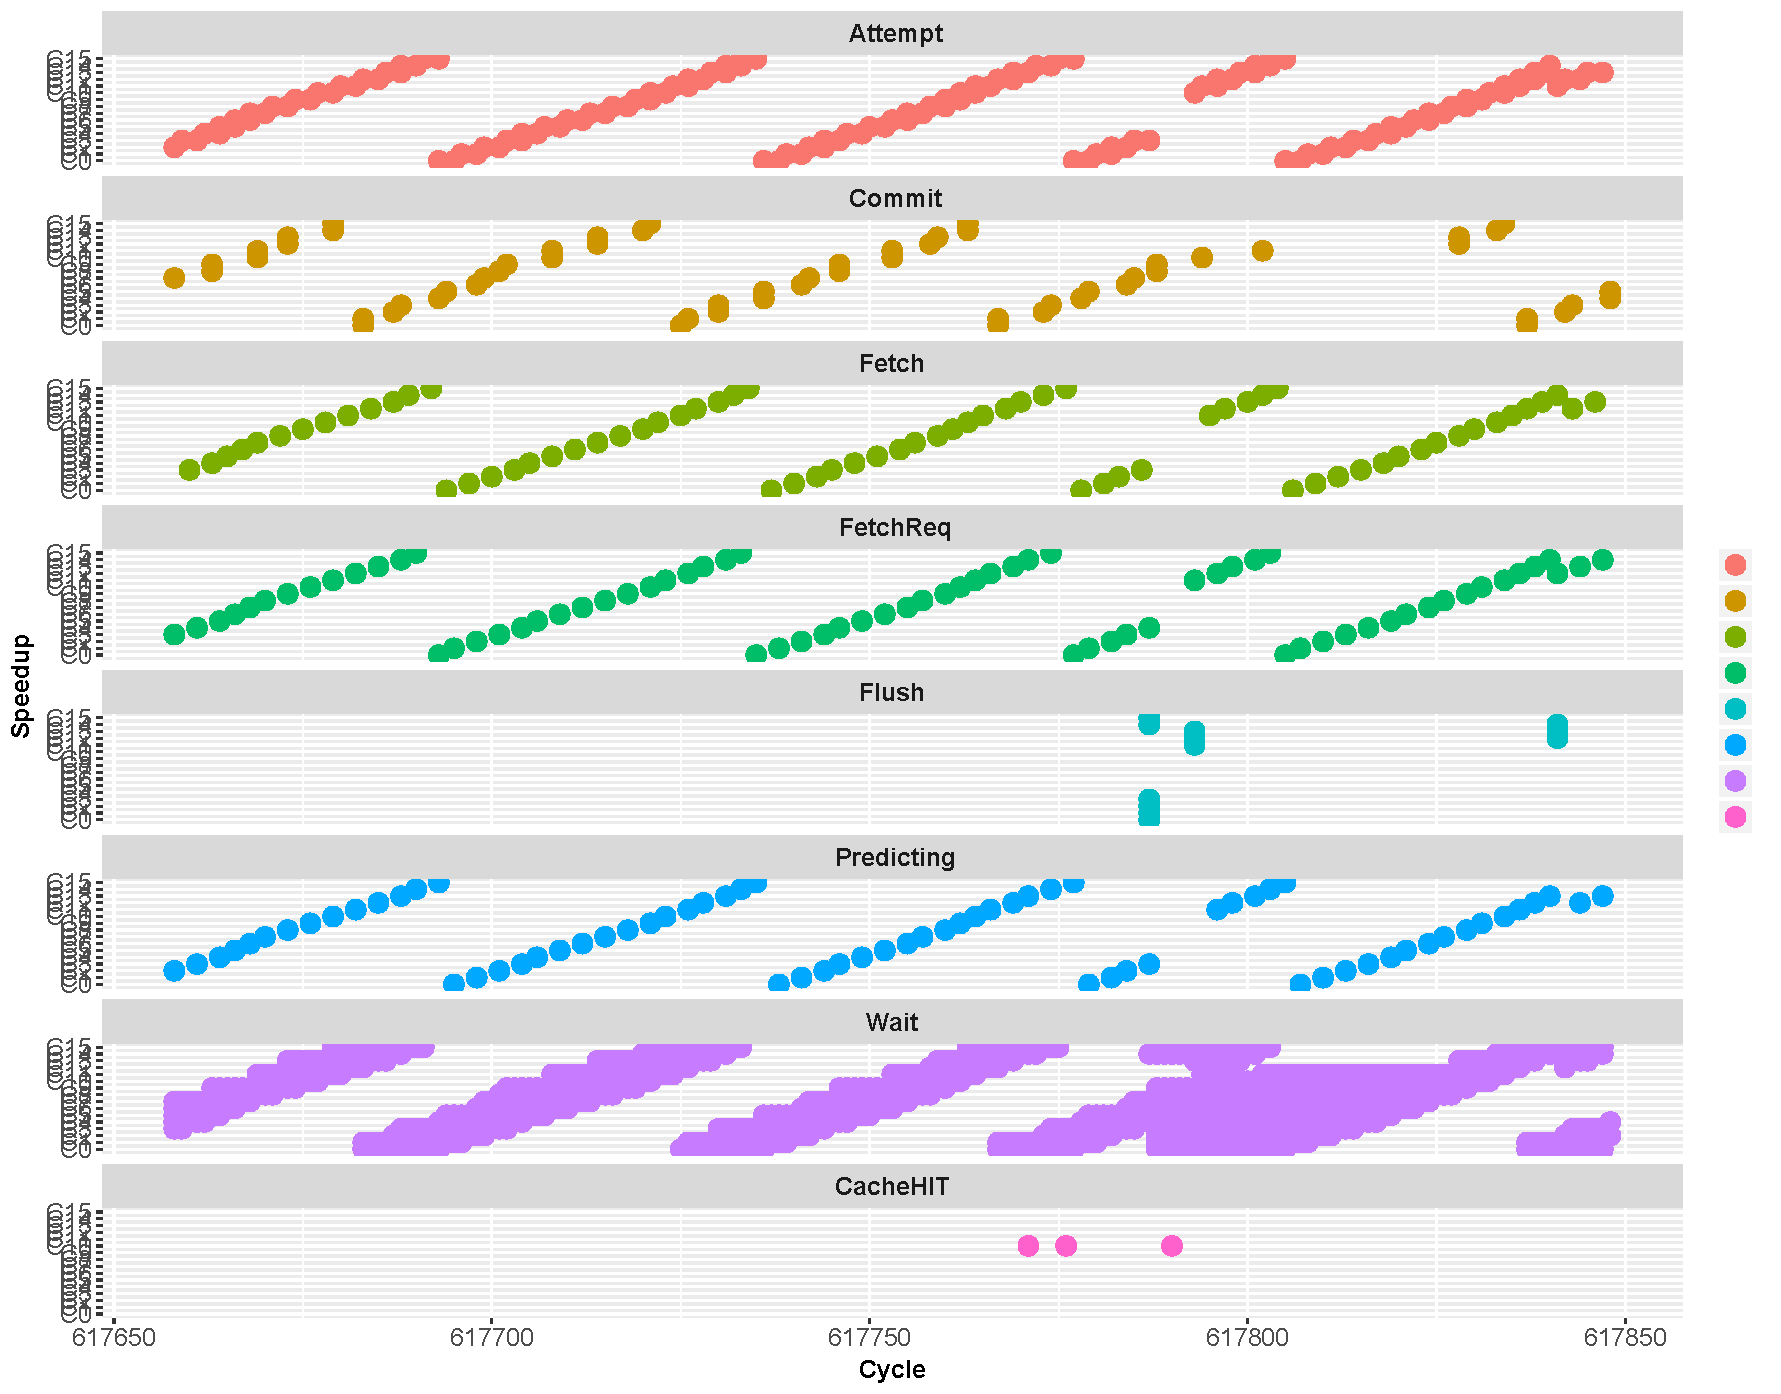
\includegraphics[width=1\textwidth]{chapter3/graphics/twolf_16_1.pdf}
  \caption{TWOLF on 16 cores fused, 1 segments each}\label{fig:16step1}
\end{figure}

\begin{figure}
\center
  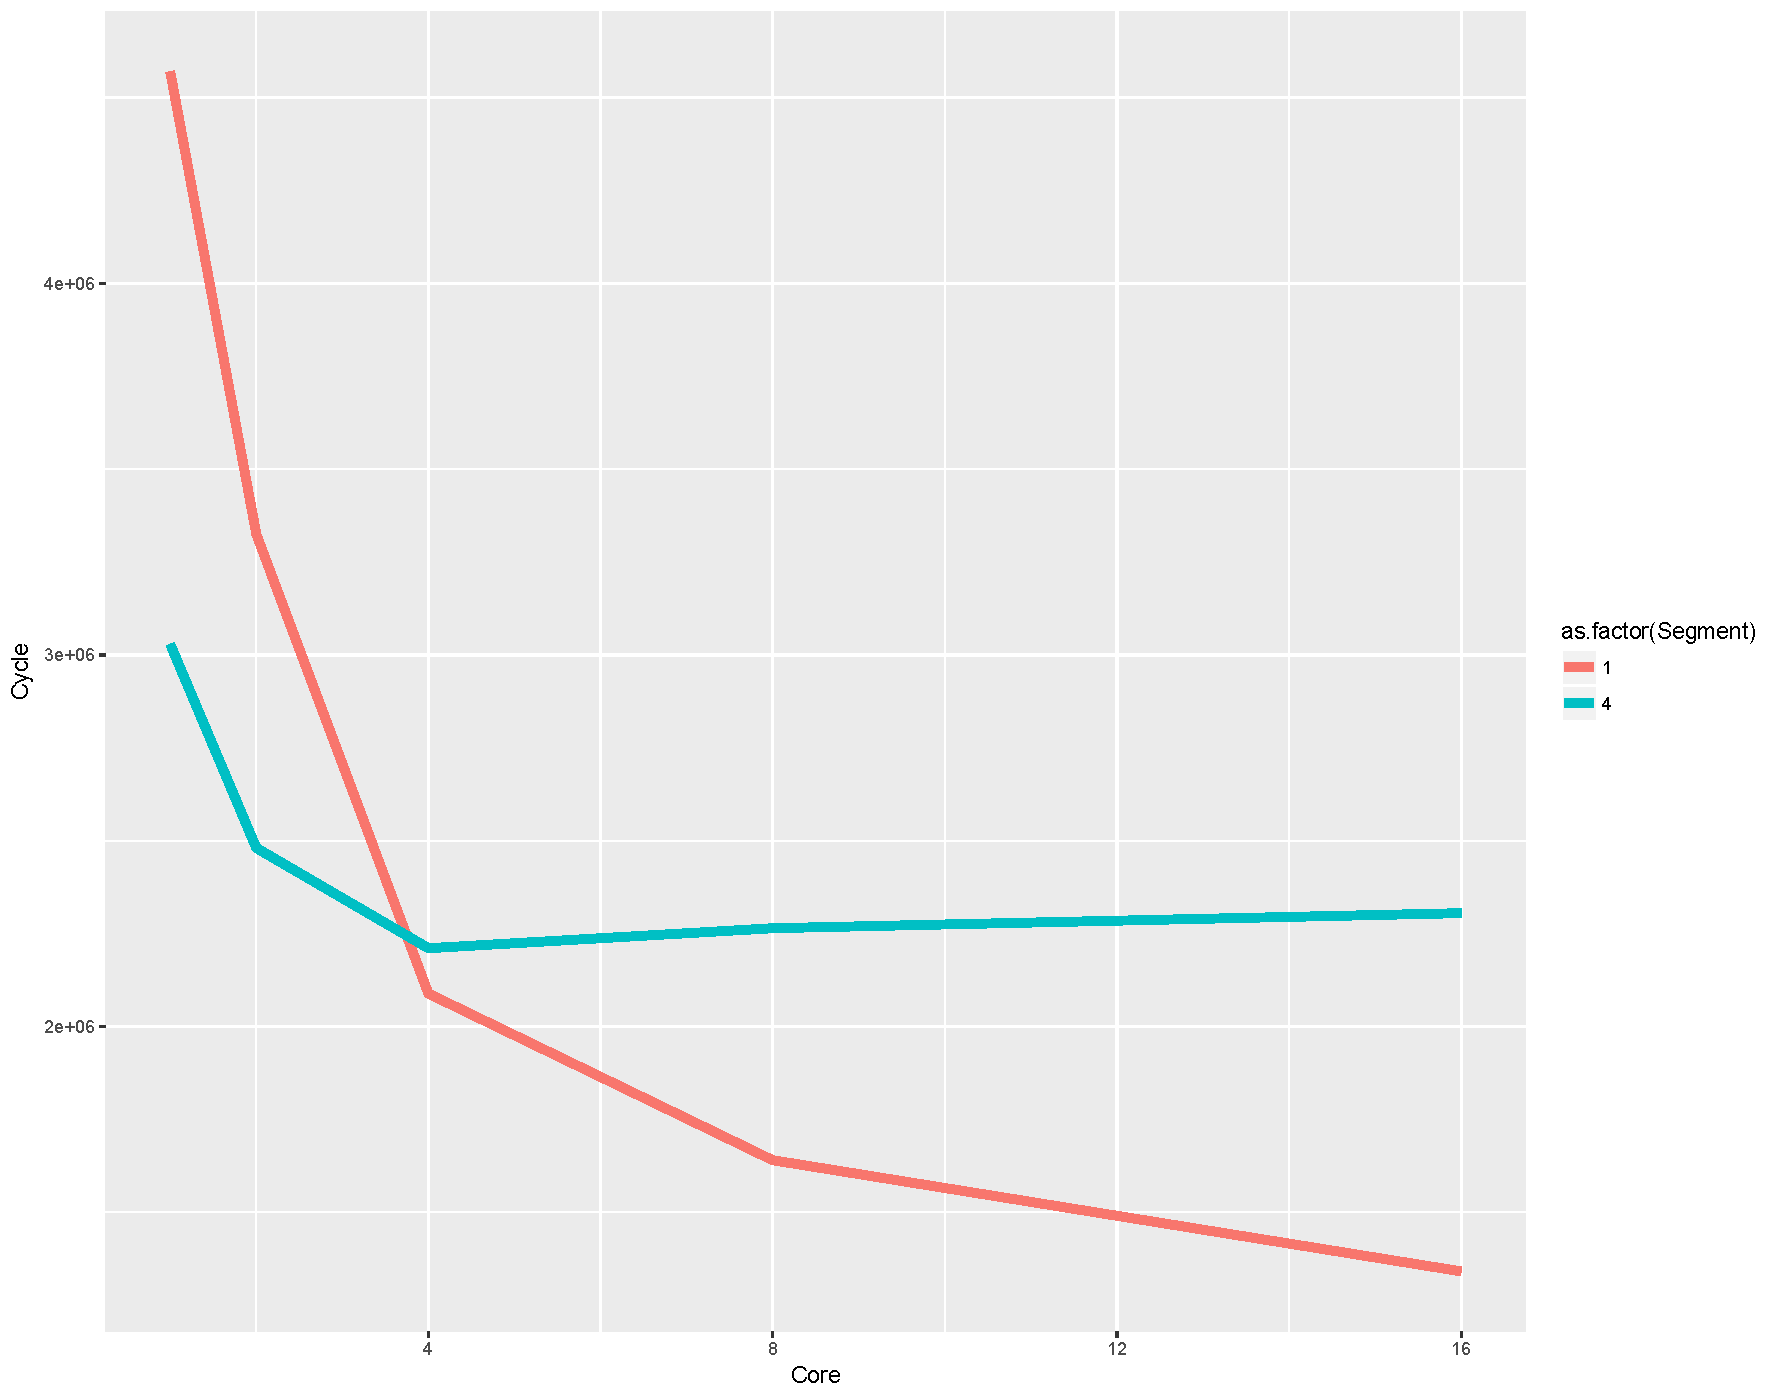
\includegraphics[width=1\textwidth]{chapter3/graphics/twolf_perf.pdf}
  \caption{Cycle comparison for 1 or 4 segments}\label{fig:4v1}
\end{figure}
Figure~\ref{fig:16step} represents the execution of 64 blocks for 16 cores fused, the Y axis represents each core, and the X axis is the cycle.
Each of the facets of the graph are defined here:
\begin{itemize}
\item Attempt: Block is attempting to allocate a new block
\item Commit:  Cycle where a block is being commited
\item Fetch: Cycle where a new block is being fetched
\item FetchReq: Cycle where a core is receiving a fetch request from another block.
\item Predicting: Cycle where a core makes a block prediction.
\item Wait: Cycle where core is in execution stage but there are no blocks in its segments.
\end{itemize}

We can clearly see how inefficient this is simply by looking at how, for almost 90% of the execution of the 64 cores, each core is simply waiting.
In fact, when looking at when cores are not waiting around, we can clearly see almost no overlap of execution between cores, meaning that the cores are never actually executing in parallel.
Since the blocks are not long enough, the overhead of fetching and dispatching blocks to multiple cores is clearly overtaking the usefulness of having this many cores.

In Figure~\ref{fig:16step1} we have an $E16_1$ running a similar section of TWOLF (getting the extact section is hard due to the difference in branching), and we can see that, when executing a single segment, the cores will have more execution time being interleaved. This is to be expected as the overhead of fetching and dispatching a single block for each core is less than 4 blocks per core.
In fact, Figure~\ref{fig:4v1} we can see that having only a single segment will outperform 4 segment cores after 4 fused cores.
The reason is once again due to how blocks are scheduled: in a single segment core, we know that each block will be executed in parallel, and each core will have a block fairly quickly.
Naturally, on a smaller cluster having 4 segments can be more advantageous as the fetch latency wont be as high.

\newpage
\subsection{Comparing segment performance}

Bear with me on this one.
In this section I want to demonstrate how average cycle count of a block affects potential speedup based on the number of segments and number of cores fused.
Unlike in CASES paper where I simply wrote a small math equation to measure maximum IPC, here I ran a small microbenchmark which contained a single instruction.
In this scenario, I could run a simulation where I could define the execution time of that instruction in cycles.
Using this, I ran a set of experiments where I modified the number of segments, 1 or 4, number of cores fused (1,2,4,8,16) and the length of the block (10,20,40,80,160,320).
I've generated 2 figures here, Figure~\ref{fig:lss} represents the speedup relative to segments.
In other words I grouped executions with the same segments to calculate the speedup.
As we can see, for a core fusion of 16 cores with 1 segment to get a 16x speedup compared to 1 core with 1 segment, we would need independent blocks of at least 40 cycles in length.
By logging fetch requests for each core, I've noticed it takes 39 cycles for 16 cores to have their blocks (in this example).
Since each block takes 40 cycles, this means that by the time Core 1 will have finished executing its block, Core 15 will have fetched and submitted a prediction.
This is an ideal situation as cores are therefore always executing blocks, leading to a full utilisation.

On 4 segment cores, the picture is much less appealing; it takes blocks of length 160 to get a 14x speedup.
By doing the same kind of logging as I did before, I see that with four segments, we take about 180 cycles to fill up all cores, so that means each block would at least have to be 180 cycles to be useful. 
Whilst this may come to no surprise, it shows that we need blocks to be at least 4x longer on a 4 segment machine compared to single segment.

So what's the point of 4 segment cores then ? It's easier to demonstrate the usefulness of core-fusion on single segment CPUs.
This may be correct, but as we can see in Figure~\ref{fig:ts} where I compare the cycle counts of all executions to 1 Core 1 Segment; having 4 segments can be very beneficial.
Indeed, on longer blocks, (160 and beyond) we could, in theory, be getting up to a 64x speedup with 16 cores and a 4x speedup with just one core!
Naturally this is purely theoretical, but there coudl be cases where this happens.
Having more segments not only should allow us to accomodate for smaller blocks, but also enables us to ensure that the cores can issue instructions at a more steady rate, as they can look for any available instruction from 4 blocks instead of a single 1.
Ironically this also shows that larger isn't always better, if we could generate 4 blocks that are perfectly independent and populate 16 cores with those blocks, we would technically get a better speedup than if we had 1 large block!

\subsubsection{Small caveat}

In this example, the block is only 1 instruction large, which makes the fetching extremeley quick.
Even though I use a perfect ICache, we have a single cycle here to fetch all the instructions needed.
I think that if the blocks are larger this will affect fetching performances (making them slower) and increasing the required length of a block.

\begin{figure}
\center
  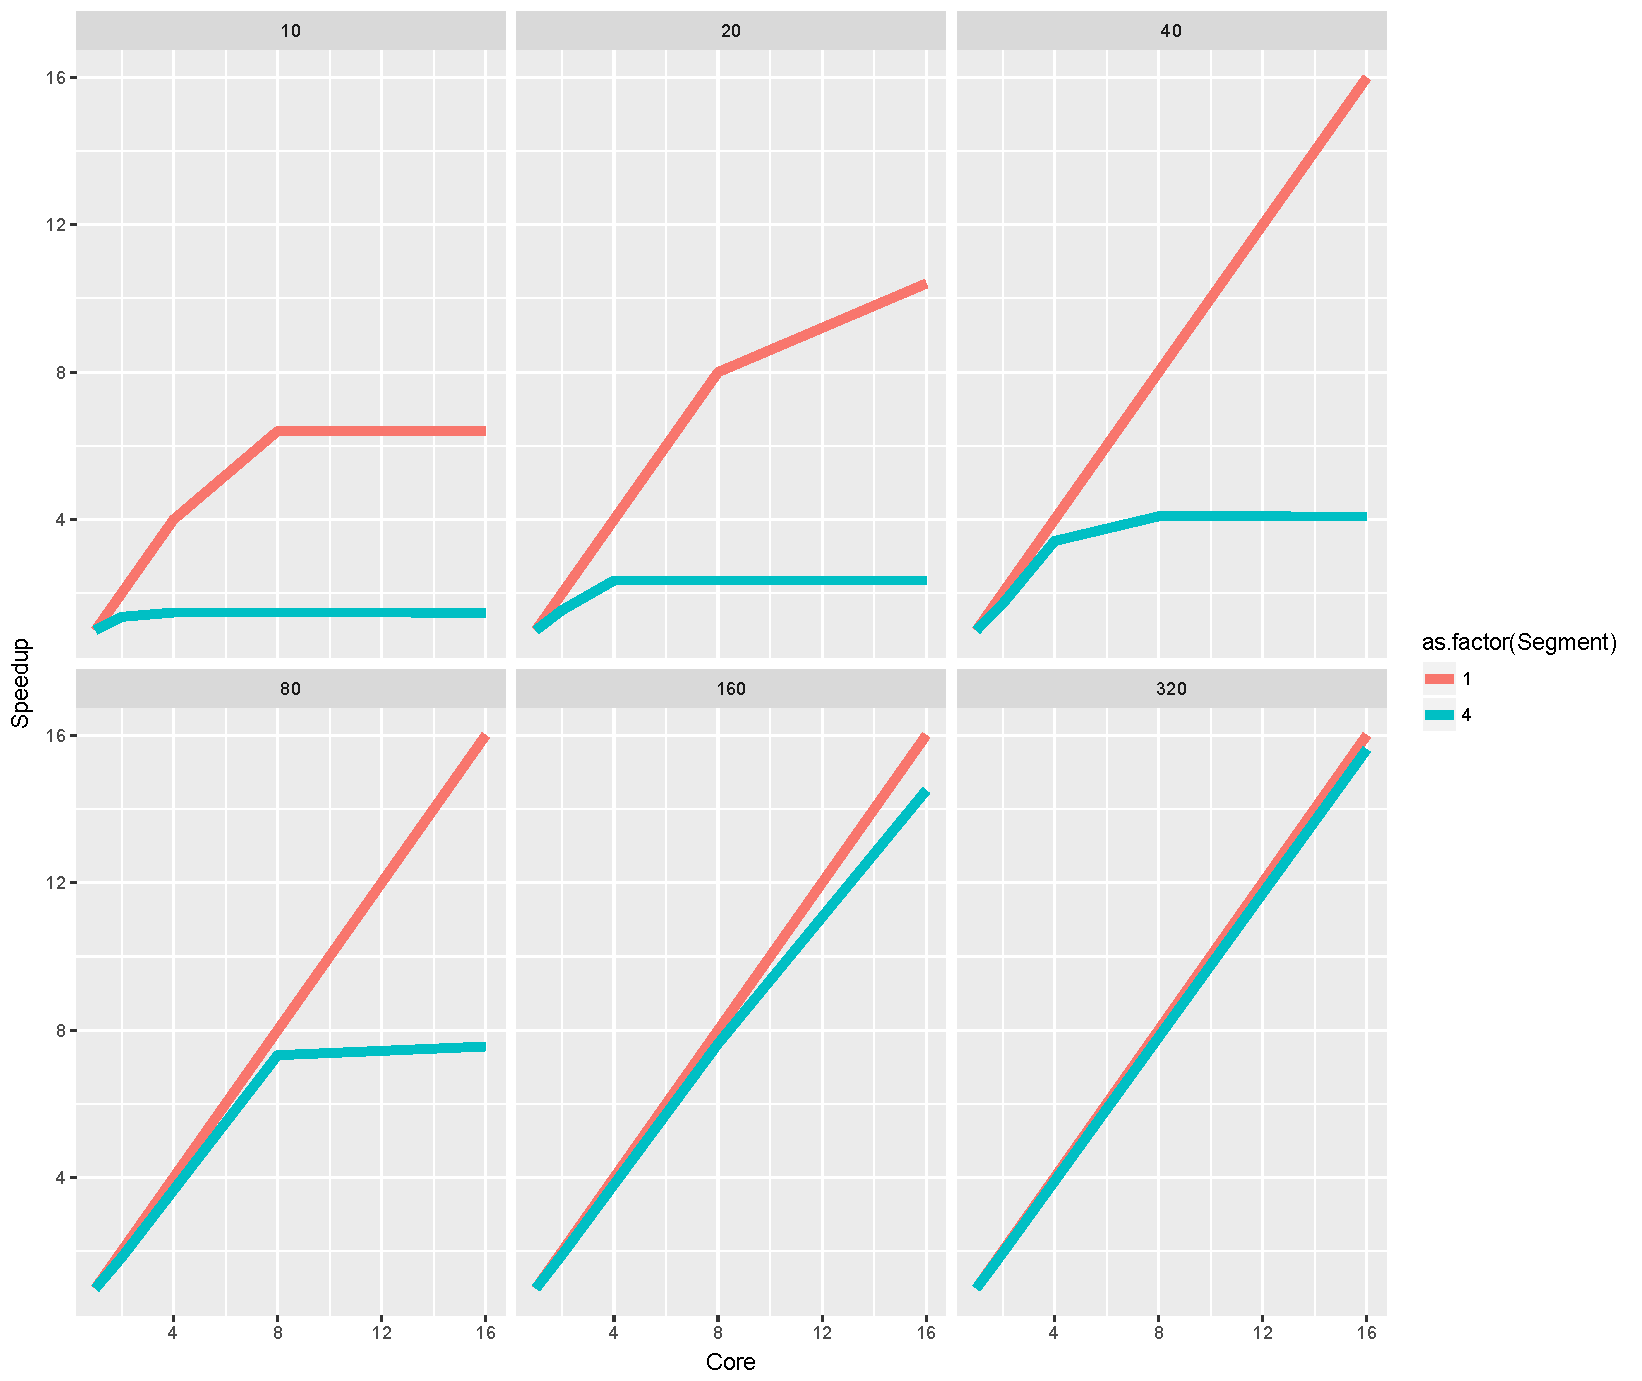
\includegraphics[width=1\textwidth]{chapter3/graphics/lengths_segment_speed.pdf}
  \caption{Speedup by segments.}\label{fig:lss}
\end{figure}

\begin{figure}
\center
  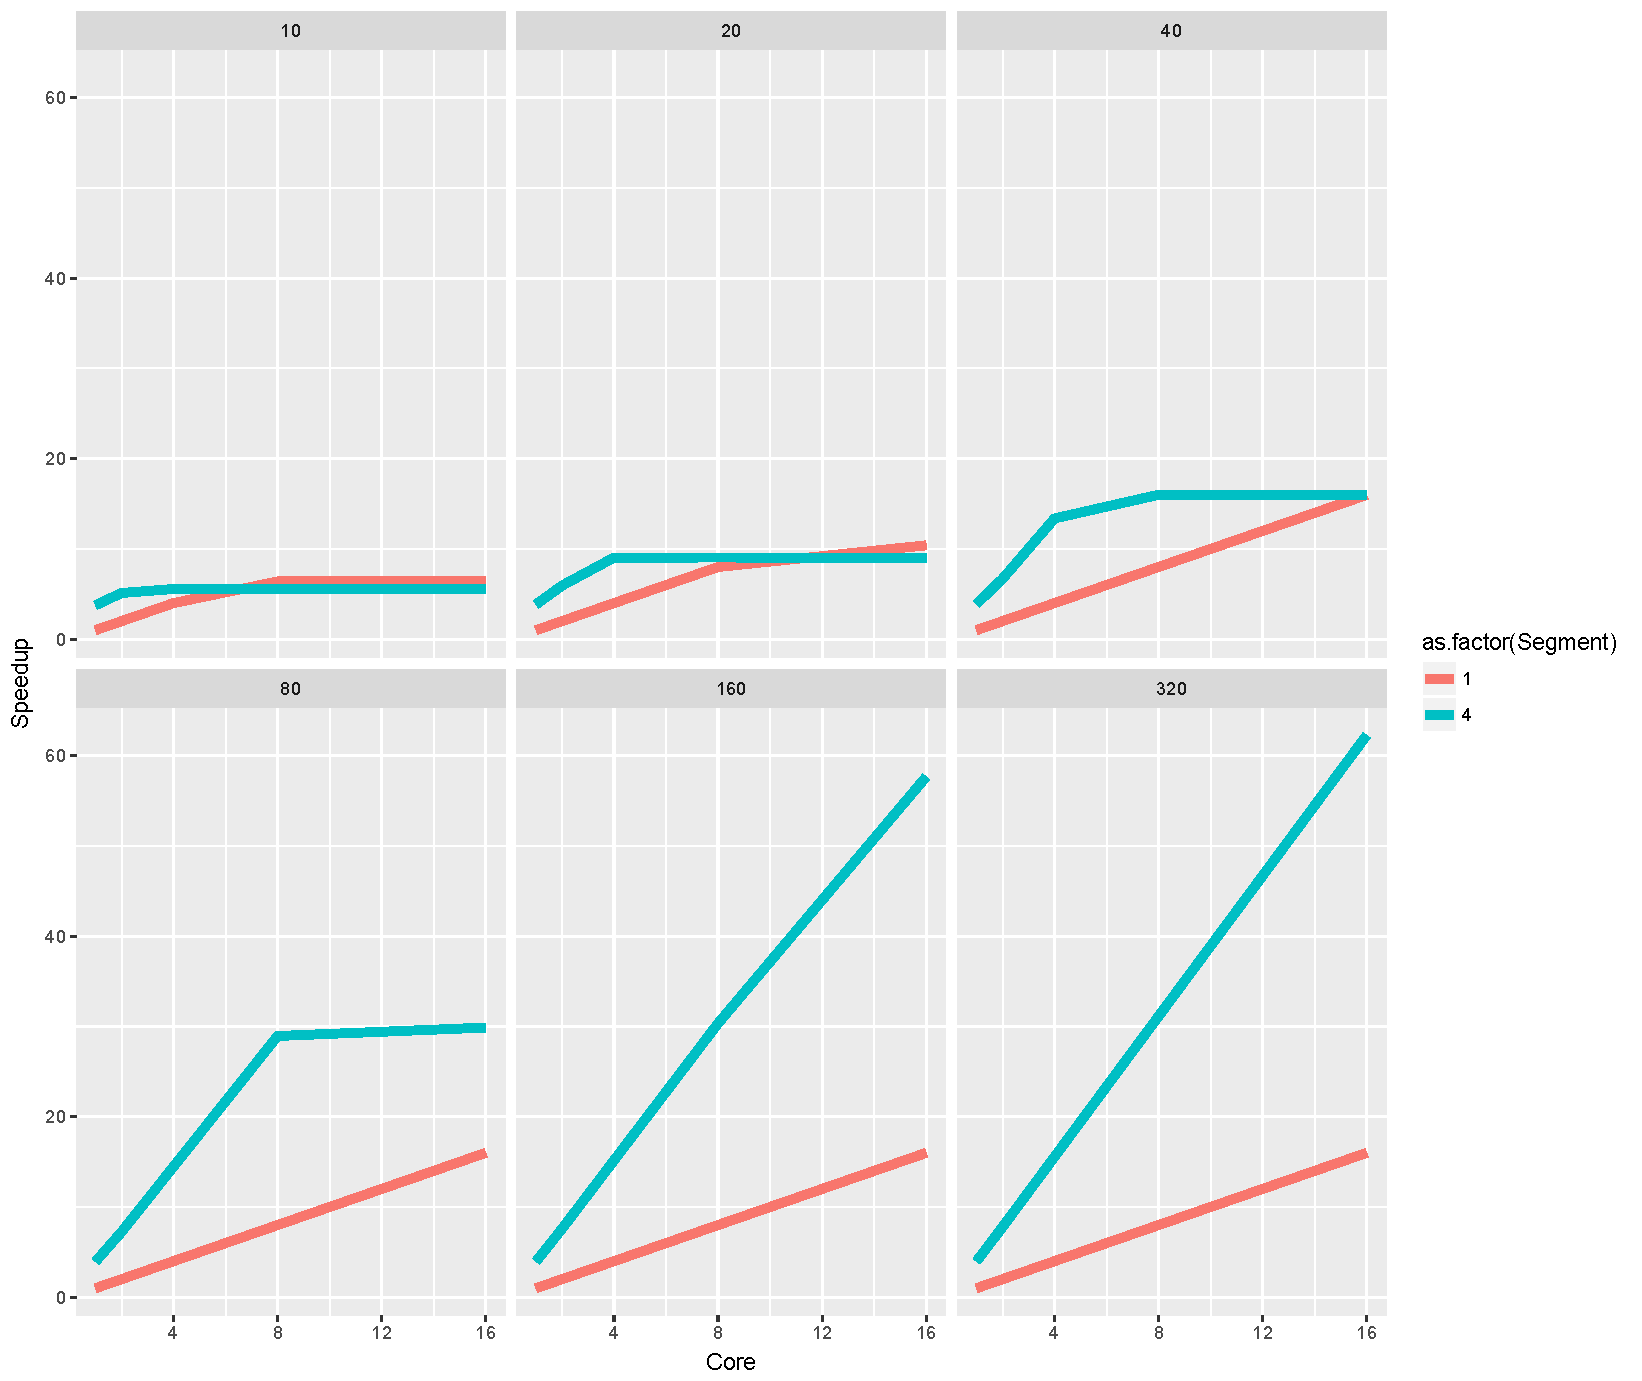
\includegraphics[width=1\textwidth]{chapter3/graphics/total_speed.pdf}
  \caption{Maximum speedup compared to 1 Core 1 Segment}\label{fig:ts}
\end{figure}


\section{How core-fusion models do it}
\subsection{EDGE}
We just described it, but again here it is:
As it exists now, each core in a composition will fetch blocks until they're full, and then submit the subsequent block to another core.
When a core no longer has the youngest segment it will wait for a core in the composition to send it a block.

\subsection{Core-Fusion, Ipek et. al}

Core-Fusion has a Fetch Management Unit (FMU) that allows it to dispatch instructions to cores in a composition.
An FMU will receive information from a core and resends relevent fetch information to other cores in the composition.
Usually the latency from 1 core to another via the FMU is 2 cycles.

In Core-Fusion, the cores independently fetch instructions from their Icache. They can fetch, at best, 2 instructions per cycle and have a max capacitiy of 8 instructions.
The cores in a fusion will be dependent on Core-Zero for fetch alignment.
When a fetch-stall occurs, such as an i-cache miss or i-tlb miss, all cores must stall to ensure correct alignment.
Each core can conduct a single prediction per cycle, it will send those predictions/mispredictions to the FMU which selects the correct PC to inform all cores about where to fetch.
A mispeculation will cause flushing of all cores, naturally.

In their situation, the overhead of fetching is supposedly negligeable, for example on an 8 Core system it's only 3\% on SPECINT/SPECFP.
However most of their time is spent in pipeline stalls, which most likely isn't alieviated by the fact that, at best, each core can only have 8 instructions running at any point.

\subsection{Baharupi, Pricopi et. al}
This is similar to EDGE but it doesn't use the block structure.
Instead, there's a "Sentinel Instruction" which acts like a block header, informing the core on whether or not the basic block ends with a branch/fallthrough.
When a core fetches a sentinel instruction it will execute a branch and submit it to the next core in the composition.
So this is similar to EDGE with single segment.
It's slightly less efficient due to the fact that the cores do live register renaming and depend on a shared General Program Counter (GPC).
Cores can't submit blocks in parallel, instead they need to lock in the GPC when they hit a sentinel instruction.
The GPC will be locked until register renaming is finished and the branch prediction is done.
This adds an extra latency as cores will simply have to wait for these procedures to be done to get ahold of the GPC.

\subsection{Conclusion}
Most core-fusion models operate in a similar manner, that is to say cores communicate with each other via some form of branch prediction / fetch manager to determine which instructions to fetch.
Baharupi introduces a lock on a General Program Counter which can cause extra latency due to cores needing to get the lock.
Core-Fusion claims to have a very small overhead, but this is also due to the fact that each core is only ever fetching a maximum of 2 instructions per cycle.
Given that they worked with an 8 core system that means they have a maximum of 64 instructions in flight at any point.
Since cores don't require a new branch prediction to fetch instructions, this can considerably reduce the overhead of the fetching model.
This is nothing compared to what EDGE can potentially do; on an 8 Core fusion we could have 1024 instructions being fetched, which could be a result of 8 to 32 fetch requests.

Ultimately EDGE requires branch predictions like Baharupi but doesn't suffer from lock-acquiring stalls.
However, unlike Core-Fusion, we cannot simply fetch instructions in parallel as we require to have decoded headers and made predictions as to what the next block will be, which increases the latency when we have more segments and cores.

\section{What can we do about it?}

\subsection{Unlocking block dispatch}

Currently a core cannot issue a new block if its youngest segment has already submitted a fetch request.
This current restriction means that blocks have to be submitted to cores in a sequential fashion, in other words, if we have 2 cores in a fusion, then C1 cannot fetch a block, send another block to C2 and then fetch a 3rd block. Instead, once it has submitted a block to C2 it will \textbf{have} to wait for C2 to send a new block.
This is what is currently causing cores to wait. Once they have submitted a block to another core, even if their youngest segment commits, they must wait for all other cores in the composition to have fetched blocks so that the fetching wraps back to it.

What I propose as a first step is to try and explore new fetching mechanisms for core-fusion, mainly pipelining fetches.
Instead of "fetching until you're full", a core should start off by making 1 prediction for itself and 1 prediction for the next core in the fusion.
Once it has executed this step it can continue fetching 3 other blocks whilst the next core repeats the process.
This should ensure all cores are fetching 4 blocks almost in parallel.
A paper from 1996 by Andre Seznec et al. from INRIA proposed a multi-block branch predictor that can generate 2 predictions in a single cycle.
We could use this work to do predictions for number of blocks.

Currently, if we have 16 cores, each fetching 4 blocks, if we assume that it takes at least 4 cycles to fetch a block and send a prediction, we have
$fetchlat=(16 * 4)*4$  so 256 cycles before each core has filled up.
By pipelining we can reduce this down to $fetchlat=4+(15*4)+4$  so 68 cycles which is a 3.7x speedup.
Refering back to Figure~\ref{fig:lss}, having an overhed of 68 cycles would place us between the 40 and 80 cycles facet, which means that if we are able to maximize speedup around those facets, that's a 2.6x speedup for a 16 core, 4 segment fusion.
This should, in theory, allow us to better utilise core-fusion as it decreases the restrictions on how long a block should take to execute for a given core-composition size.
Let's recall in the previous report that the overall speedup of a loop, when we only have a single segment can be measured by:
\begin{equation}\label{eq:avspeed}
\frac{Average Execution Time}{\frac{4+4*(Cores -1)+ Average Execution Time + Dependencies  * Cores}{ Cores}}
\end{equation}

In this formula, $4+4*(Cores-1)$ represents the fetch overhead when we have a single segment.
Currently, on 4 segments this would be $4+4*(Cores-1)*4$ which reduces the potential speedup window.

\subsection{Improving branch prediction requirements}

We can use this oportunity of exploring how blocks are fetched to improve overall core-utilisation by ordering the blocks in a different manner.
As we state in the CASES paper, for a core to be useful in a core-fusion, all previous blocks must have been accurately predicted, which can be a huge strain on the branch predictor.
If, instead, we were to send the first prediction made by a core to the following core, we can reduce the stress on the branch predictor.
For example if we had 4 Cores, C1 would have blocks [1,5,9,13] C2:[2,6,10,14], C3:[3,7,11,15] and C4:[4,8,12,16].
In this case, we only need to make 3 predictions to ensure that C4 has at least been somewhat useful.
Previously, in a 16 core composition, if we had 64 blocks in flight, the 16th core could only be considered useful if 60 out of the 64 blocks were considered correct.
This implied at least a 93.7\% accuracy just to ensure that all cores were running some correct code whereas in this new model, only 15 predictions would ensure a utilisation of the core, so dropping it to a mere 23\%.
In Core-Fusion by Ipek et al. Figure 9 shows the distribution of fetch cycles for SPECINT and SPECFP benchmarks.
They define 4 categories: pipeline stalls (cores are busy executing), wrong path (misprediction), FMU stalls (stalls caused by communicating to FMU) and true fetch, which I assume is cycles spent doing actual fetch work.
Whilst they claim that the FMU only causes a 3\% overhead in fetch cycles, they fail to address the fact that, for some benchmarks in SPECINT, mispeculation can caust them up to 50\% of their fetch cycles which is huge.
In these cases they percieve no speedup since they're getting branches wrong almost half the time.
By changing the scheme we can claim that we maintain a higher number of live blocks whilst allowing cores to be useful more frequently.

\subsection{Exploring smarter schedulers}

A lot of the talk in this report is somewhat focused on trying to tackle fetching overhead when we assume blocks are small and take no time to execute.
This most often will only occur in integer heavy blocks, or situations where all data is in cache and blocks are small due to heavy control flow.
However this isn't always the case, and blocks can take a long time to execute.
In these situations, the overhead of fetching isn't the problem but rather which blocks are being fetched and dispatched.
Since we're playing around with how blocks are dispatched we may use this oportunity to look at loops 

%% !TEX TS-program = pdflatex
% !TEX encoding = UTF-8 Unicode

% This is a simple template for a LaTeX document using the "article" class.
% See "book", "report", "letter" for other types of document.

\title{Understanding fetching performance on a core-fusion enabled processor}
\section{Introduction}
I want to discuss what affects overall performance in a core-fusion based on how cores fetch blocks in a core-fusion.
I'll start by describing how fetching works on core-fusion when there's only a single segment, this will be followed by how this is expanded on when we enable 4 segments per core.
Next I'll cover 2 different processors that also use core-fusion; Ipek et al.'s original Core-Fusion processor and Pricopi et al.'s Baharupi.
Once the background is all covered I'll demonstrate how different instruction block parameters will influence the overall performance of a core composition.
This involves discussing block size in terms of bytes, instructions and cycle lengths.
We'll also see how the number of segments will require different types of blocks to be maximize performance.
With all this information at hand we then pose the question of how scheduling blocks in a different order may improve performane (getting lower cycle counts), but also may help alleviate  branch prediction requirements.

\section{Setup}
In this article we assume a 16 core processor with either 1 or 4 segments per core.
A segment represents the number of blocks a core can fetch and execute in parallel, which, in EDGE will be: $128/NumberOfSegments$.
The information in the rest of the article is based on the simulator implementation, some of this can be potentially changed, but for now we're focussing on what's implemented.
To facilitate the explanations I assume a perfect instruction cache.

\section{Understanding the fetching procedure}
The fetch procedure can be broken up into 4 steps.

\begin{itemize}
\item Step 1: Fetch block header and decode it. This will give us block size, number of instructions and the address needed to make prediction.
\item Step 2: Make ICache fetch requests to fetch block.
\item Step 3: Make branch prediction.
\item Step 4: Once the branch prediction is done, see if we can make a request for a new block.
\end{itemize}

In the simulator, steps 2, 3 and 4 can potentially be done in the same cycle. We need at least 1 cycle to fetch and decode the header, and step 4 has to be done at least 1 cycle after the prediction.

\textbf{SIMULATOR NOTE}: In the simulator, there is a current condition that states that a new block can only be fetched once a previous block has finished fetching. We will discuss later on in the report how this affects performance.
The original E2 paper does not specify that blocks will be fetched in parallel and a comment in the code claims that they don't track segment fetches in parallel (hence the waiting condition).

\subsection{Fetching on a core composition}.

When cores are fused, this changes the fetching mechanics slightly.
To simplify the explanation I will redefine every step, this time when cores are fused.


\begin{itemize}
\item Step 1: Fetch block header and decode it. This will give us block size, number of instructions and the address needed to make prediction.
\item Step 2: Make ICache fetch requests to fetch block.
\item Step 3: Make branch prediction.
\item Step 4: Once the branch prediction is done, see if we can make a request for a new block.
\item Step 5: If we cannot fit the newly predicted block on our core, send a fetch request in the composition.
\end{itemize}

There is only one new step in the composition version, however, in the current setup we will see a new restriction.
The new restriction is: If you do not hold the youngest block in one of your segments then you may no longer make fetch requests.
This means that cores in a composition are not fully autonomous, they will have to wait for another core in the composition to send them a fetch signal before being able to fetch blocks.
We will see later on how that affects performance.

\section{Related architectures}

\subsection{Core-Fusion, Ipek et. al}

Core-Fusion has a Fetch Management Unit (FMU) that allows it to dispatch instructions to cores in a composition.
An FMU will receive information from a core and resends relevent fetch information to other cores in the composition.
Usually the latency from 1 core to another via the FMU is 2 cycles.

In Core-Fusion, the cores independently fetch instructions from their Icache. They can fetch, at best, 2 instructions per cycle and have a max capacitiy of 8 instructions.
The cores in a fusion will be dependent on Core-Zero for fetch alignment.
When a fetch-stall occurs, such as an i-cache miss or i-tlb miss, all cores must stall to ensure correct alignment.
Each core can conduct a single prediction per cycle, it will send those predictions/mispredictions to the FMU which selects the correct PC to inform all cores about where to fetch.
A mispeculation will cause flushing of all cores, naturally.

In their situation, the overhead of fetching is supposedly negligeable, for example on an 8 Core system it's only 3\% on SPECINT/SPECFP.
However most of their time is spent in pipeline stalls, which most likely isn't alieviated by the fact that, at best, each core can only have 8 instructions running at any point.

\subsection{Baharupi, Pricopi et. al}
This is similar to EDGE but it doesn't use the block structure.
Instead, there's a "Sentinel Instruction" which acts like a block header, informing the core on whether or not the basic block ends with a branch/fallthrough.
When a core fetches a sentinel instruction it will execute a branch and submit it to the next core in the composition.
So this is similar to EDGE with single segment.
It's slightly less efficient due to the fact that the cores do live register renaming and depend on a shared General Program Counter (GPC).
Cores can't submit blocks in parallel, instead they need to lock in the GPC when they hit a sentinel instruction.
The GPC will be locked until register renaming is finished and the branch prediction is done.
This adds an extra latency as cores will simply have to wait for these procedures to be done to get ahold of the GPC.

\subsection{Conclusion}
Most core-fusion models operate in a similar manner, that is to say cores communicate with each other via some form of branch prediction / fetch manager to determine which instructions to fetch.
Baharupi introduces a lock on a General Program Counter which can cause extra latency due to cores needing to get the lock.
Core-Fusion claims to have a very small overhead, but this is also due to the fact that each core is only ever fetching a maximum of 2 instructions per cycle.
Given that they worked with an 8 core system that means they have a maximum of 64 instructions in flight at any point.
Since cores don't require a new branch prediction to fetch instructions, this can considerably reduce the overhead of the fetching model.
This is nothing compared to what EDGE can potentially do; on an 8 Core fusion we could have 1024 instructions being fetched, which could be a result of 8 to 32 fetch requests.

Ultimately EDGE requires branch predictions like Baharupi but doesn't suffer from lock-acquiring stalls.
However, unlike Core-Fusion, we cannot simply fetch instructions in parallel as we require to have decoded headers and made predictions as to what the next block will be, which increases the latency when we have more segments and cores.

\section{On Performance}
\subsection{Motivating example}
To start things off, I want to motivate how crucial a good fetching policy is, and how the current policies regarding fetching in a core composition can penalise performance.
In this subsection I am executing a twolf\_1 microbenchmark, which involves a loop with a set of very small blocks. 
This ensures that for the most part, each core can fetch 4 blocks.
To understand how the current fetching policy affects composition performance I track specific events that happen in the processor.
These events are:
\begin{itemize}
\item The first cycle that we fetch a new block \textbf{Fetch}.
\item The cycle at which we make a prediction for the next block \textbf{Predict}.
\item The cycle at which we make an attempt to allocate a new block \textbf{Attempt}.
\item The cycle at which a core makes a fetch request to  another core \textbf{FetchReq}.
\item The cycle at which we have to flush blocks \textbf{Flush}.
\item Cycle in which the core has no blocks and is waiting \textbf{Wait}.
\end{itemize}
Figure~\ref{fig:16step} represents a slice of the twolf\_1 execution on a 16 core, 4 segment processor.
The X axis represents the cycle count and the Y axis represents a core in the composition.
Each facet represents one of the previously mentioned events, and thus, a dot represents when one of the cores in the composition logged an event, and which cycle that happened on.

The important aspects to notice are: how the fetch requests form a stair shape, which shows how long it takes for every core to be full.
This stair shape is, of course, caused by the serialisation of the block fetches and the fact that a core only starts fetching blocks once the previous core has made a request.
The second crucial bit of information is noticing how dense the Wait facet is.
As we can see, cores spend far more time waiting than they do actualy executing code.
This is due to the fact that once they have committed their blocks, they won't be provided new blocks until its parent core submits a request.
Also, looking at when cores \textbf{do} execute code, we can see that this is barely done in parallel. 
This means that the improvements expected of core-fusion are not present in this example, as the work is serialised.


Figure~\ref{fig:16step1} represents a similar slice of the twolf\_1 microbenchmark, except this time we have 16 cores fused with a single segment.
We can ignore the CacheHit event as this is not relevant in this section.
As we can see, when each core only has a single segment, it takes less time for the composition to fill up with blocks, and thus, when looking at the Wait facet, more code is being executed in parallel.
Naturally, this is due to the fact that in a single segment processor, we can only have 16 blocks in flight, compared to the 4 segment's 64, thus the overhead of fetching is reduced.
Whilst this facilitates the motivation of core fusion, having a single segment core is a waste of resources as often times the compiler will never generate blocks of 96 instructions or more.

\begin{figure}
\center
  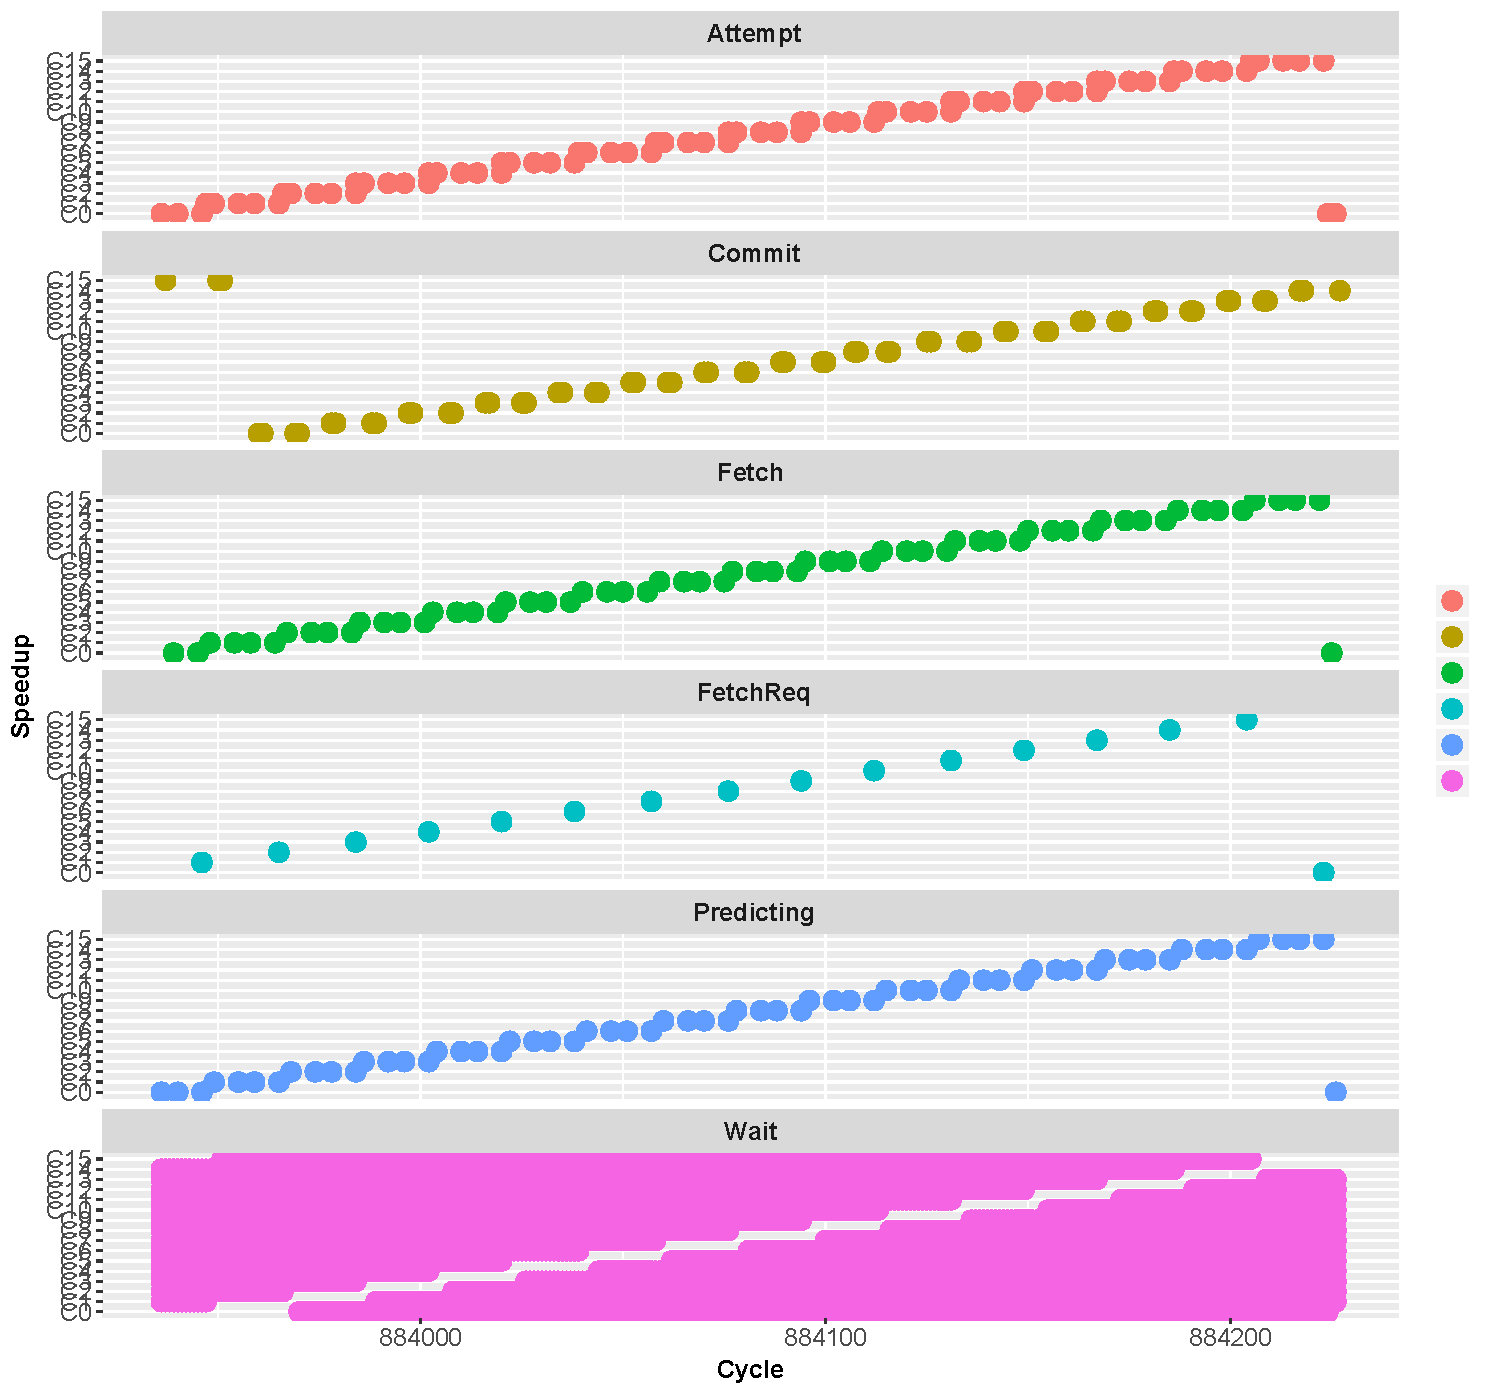
\includegraphics[width=1\textwidth]{chapter3/graphics/twolf_16.pdf}
  \caption{TWOLF on 16 cores fused, 4 segments each}\label{fig:16step}
\end{figure}

\begin{figure}
\center
  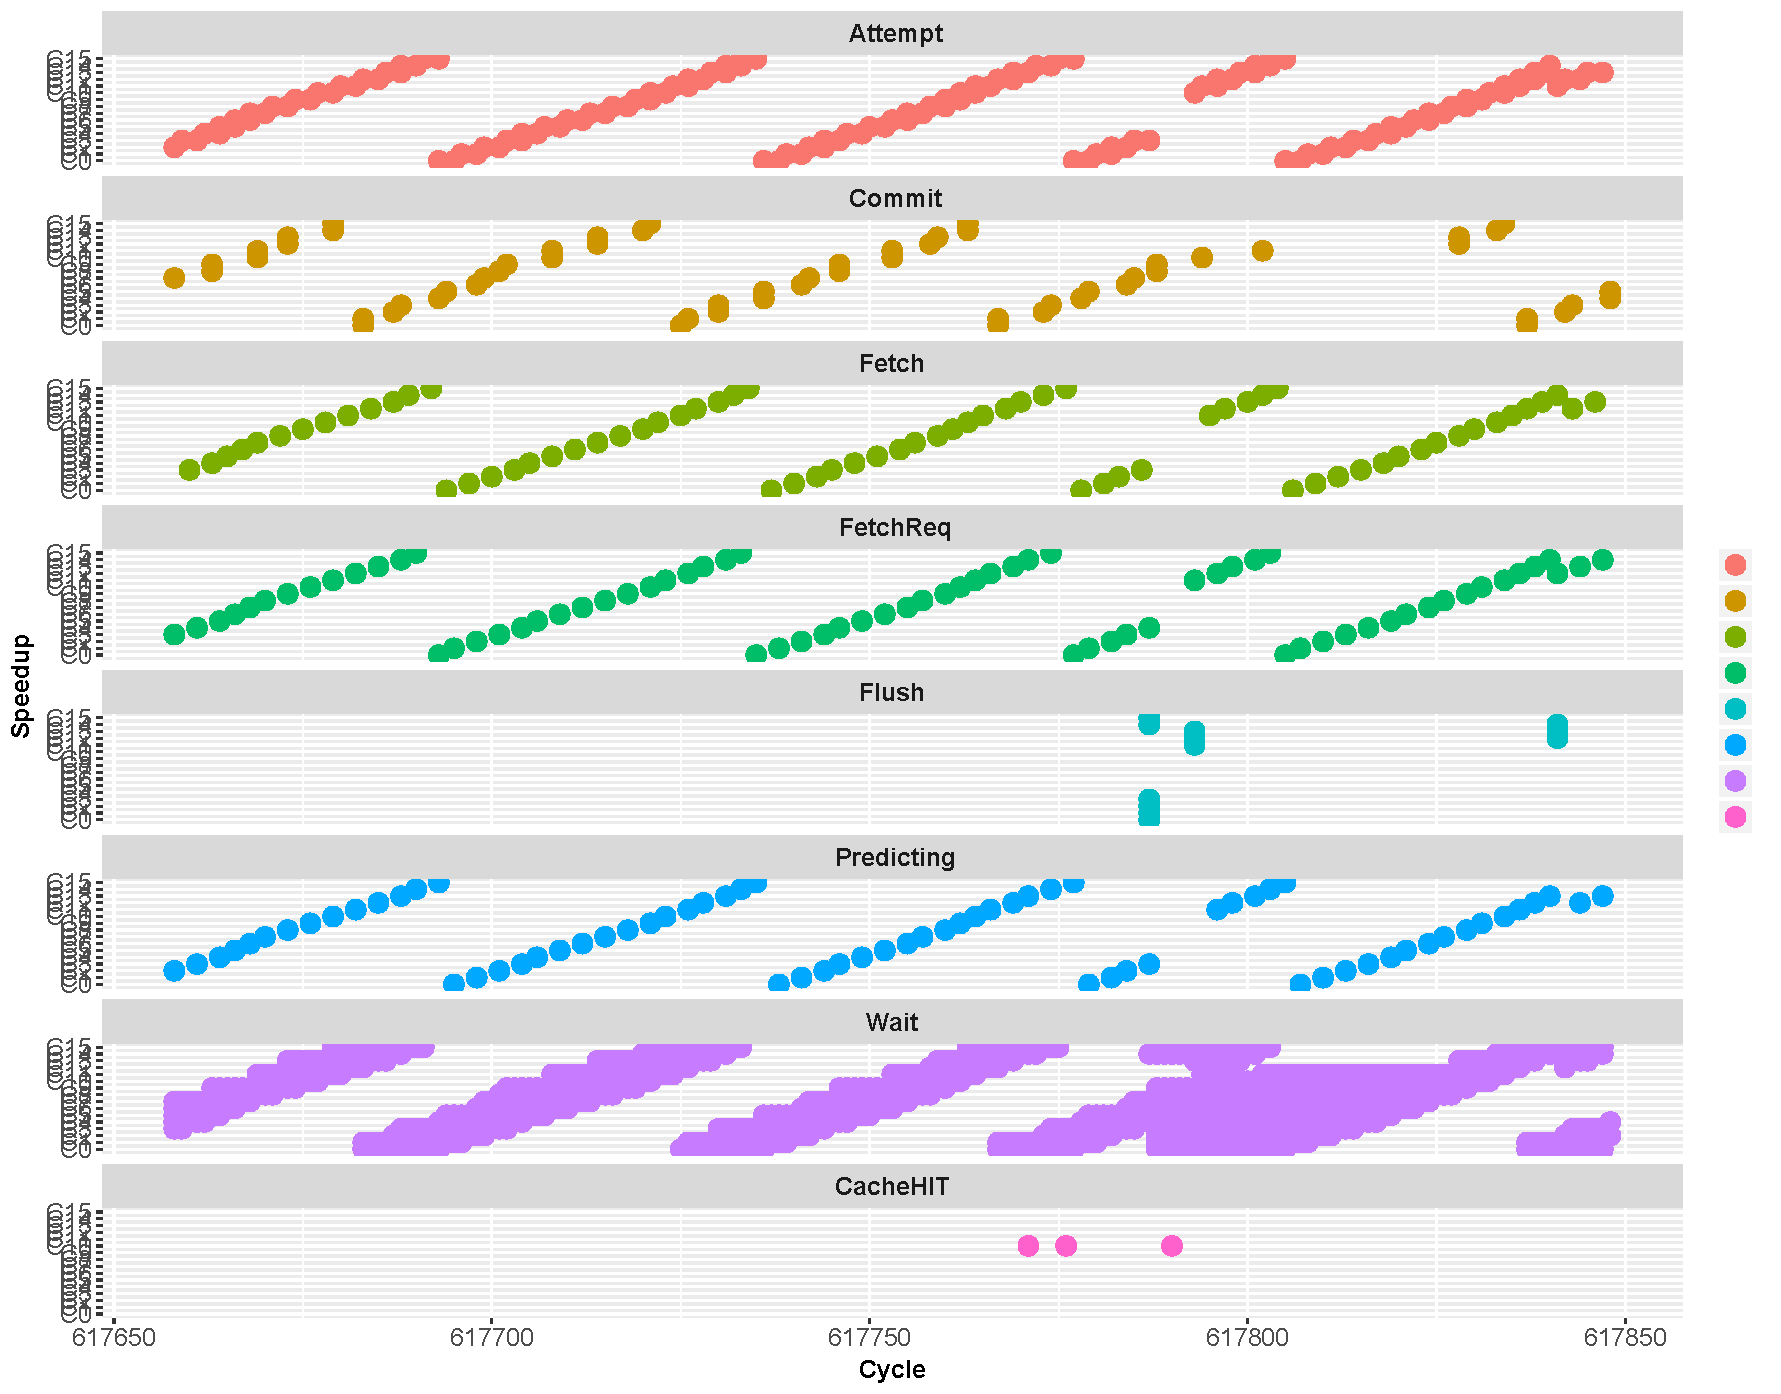
\includegraphics[width=1\textwidth]{chapter3/graphics/twolf_16_1.pdf}
  \caption{TWOLF on 16 cores fused, 1 segments each}\label{fig:16step1}
\end{figure}
\newpage
\subsection{Using synthetic benchmarks}
In the CASES paper I provided a small model to try and understand when a composition could be fully utilised in terms of IPC through the study of instructions per block.
Here we will do a study based on the actual cycle counts from different synthetic benchmarks.

\subsection{Comparing segment performance based on small blocks}
In this section I want to demonstrate how the average time it takes to execute a block in cycles affects potential speedup based on the number of segments and number of cores fused. 
In this scenario, I run a simulation where I define a block with a single instruction and manually assign the execution time of that instruction.
The blocks are independent, allowing for cores in a composition to execute in parallel.
I ran a set of experiments where I modified the number of segments, 1 or 4, number of cores fused (1,2,4,8,16) and the execution time of the block of the block (10,20,40,80,160,320 cycles).
Figure~\ref{fig:lss} represents the speedup obtained via core-fusion fusion relative to their segment count (so comparing cycle count of 1 core 1 segment with 16 core 1 segment for example).

As we can see, for a core fusion of 16 cores with 1 segment to get a 16x speedup we need independent blocks of at least 40 cycles in length.
By logging fetch requests for each core, I've noticed it takes 39 cycles for 16 cores to have a block to execute (in this example).
This is due to the fact that it takes 2 cycles to fetch header, make prediction, and send a request to another core + some extra cycles to fully fetch the block.
Since each block takes 40 cycles, this means that by the time Core 1 will have finished executing its block, Core 16 will have fetched its block and submitted a prediction and therefore Core 1 can immediately fetch a new block.
This is an ideal situation as cores are therefore always executing blocks, leading to a full utilisation.

On 4 segment cores, the picture is much less appealing; it requires blocks to take at least 160 cycles to get a 14x speedup compared to 1 Core with 4 segments.
By doing the same kind of logging as I did before, I see that with four segments, we take about 180 cycles to fill up all cores, so that means each block would at least have to be 180 cycles to be fully useful. 
Whilst this may come to no surprise, it shows that we need blocks to be at least 4x longer on a 4 segment machine compared to single segment.

So what's the point of 4 segment cores then ? It's easier to demonstrate the usefulness of core-fusion on single segment processors than it is on 4 segments.
This may be correct, but as we can see in Figure~\ref{fig:ts} where I compare the cycle counts of all executions to 1 Core 1 Segment; having 4 segments can be very beneficial.
Indeed, on longer blocks, (160 and beyond) we could, in theory, be getting up to a 64x speedup with 16 cores and a 4x speedup with just one core!
Naturally this test is synthetic, but there coudl be cases where this happens.
Having more segments not only should allow us to accomodate for smaller blocks, but also enables us to ensure that the cores can issue instructions at a more steady rate, as they can look for any available instruction from 4 blocks instead of a single 1.
Ironically this also shows that larger isn't always better, if we could generate 4 blocks that are perfectly independent and populate 16 cores with those blocks, we would technically get a better speedup than if we had 1 large block!

\begin{figure}
\center
  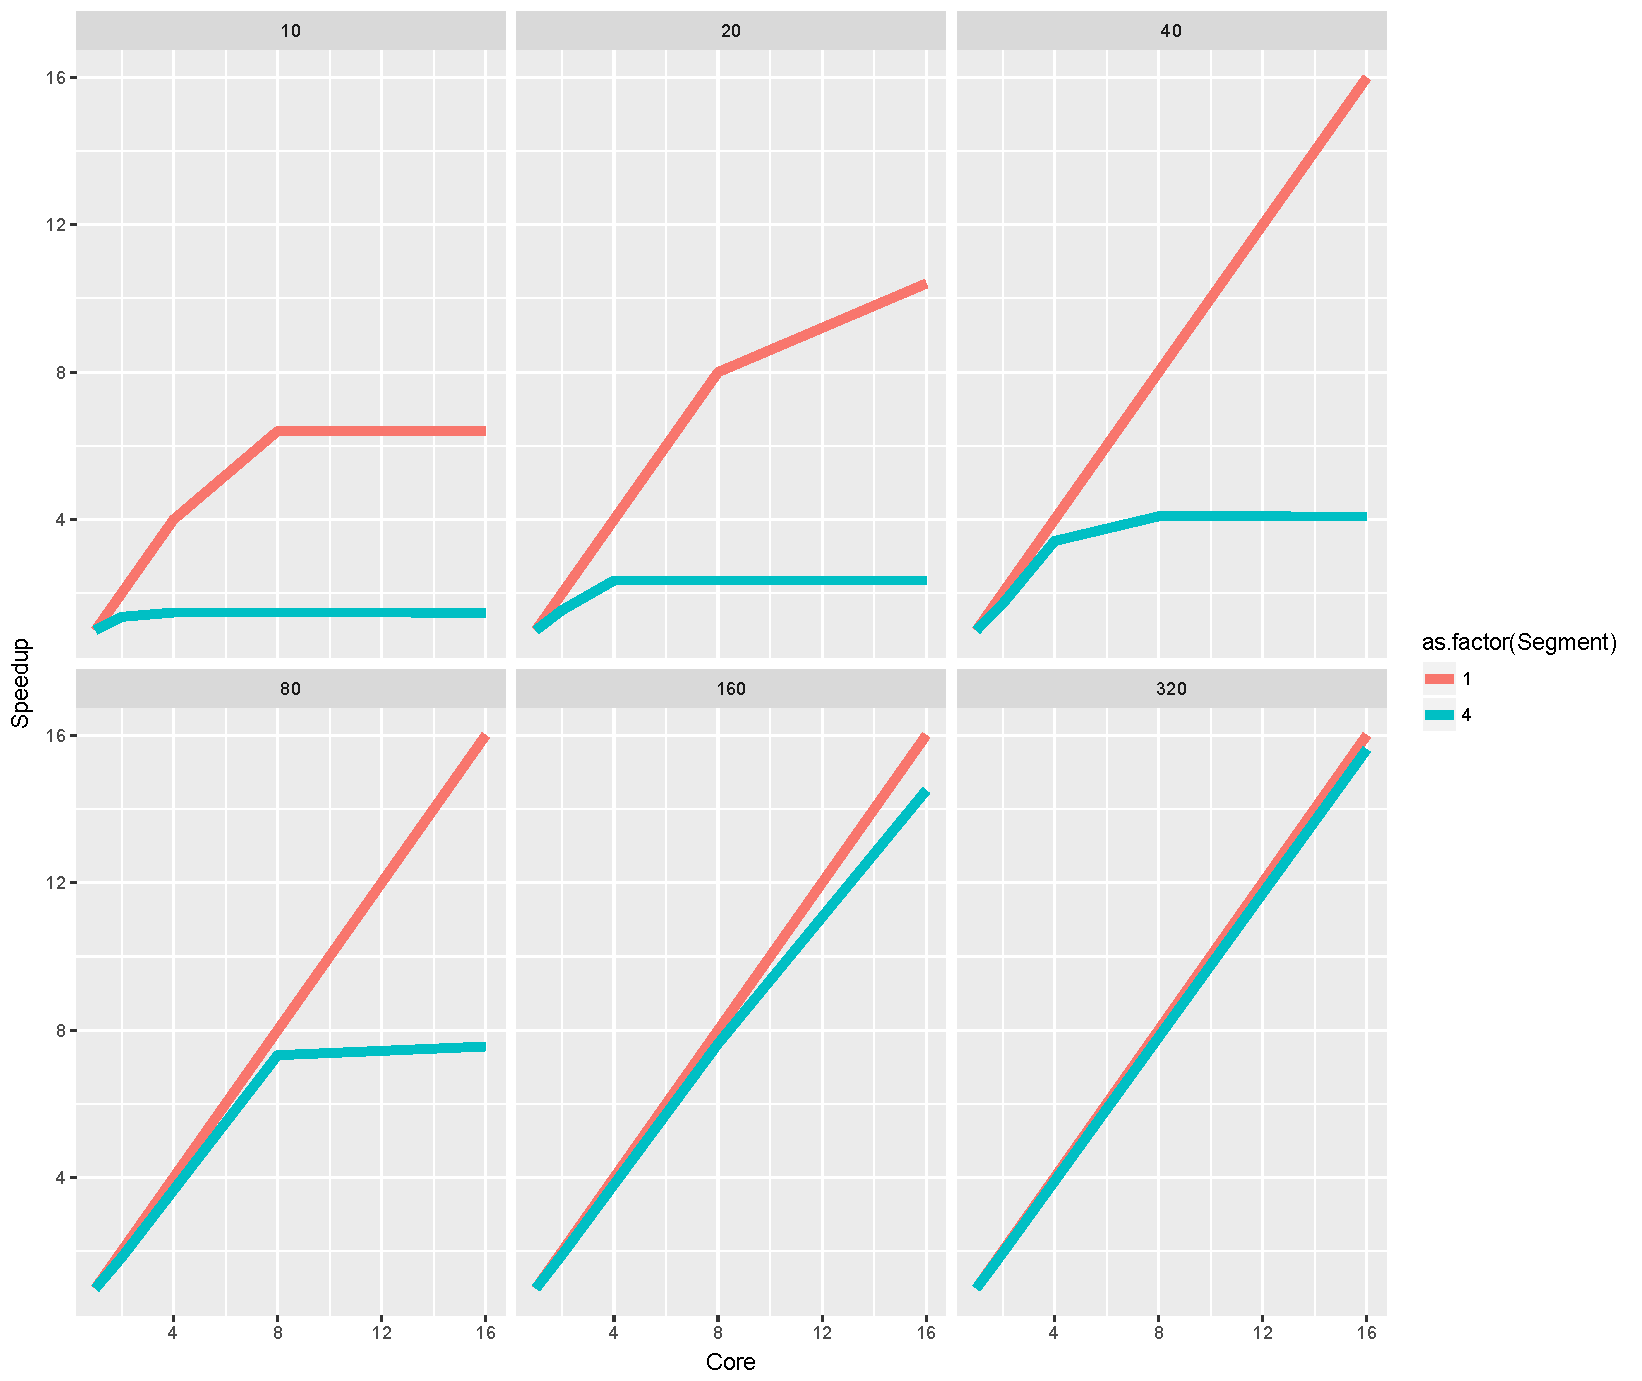
\includegraphics[width=1\textwidth]{chapter3/graphics/lengths_segment_speed.pdf}
  \caption{Speedup by segments.}\label{fig:lss}
\end{figure}

\begin{figure}
\center
  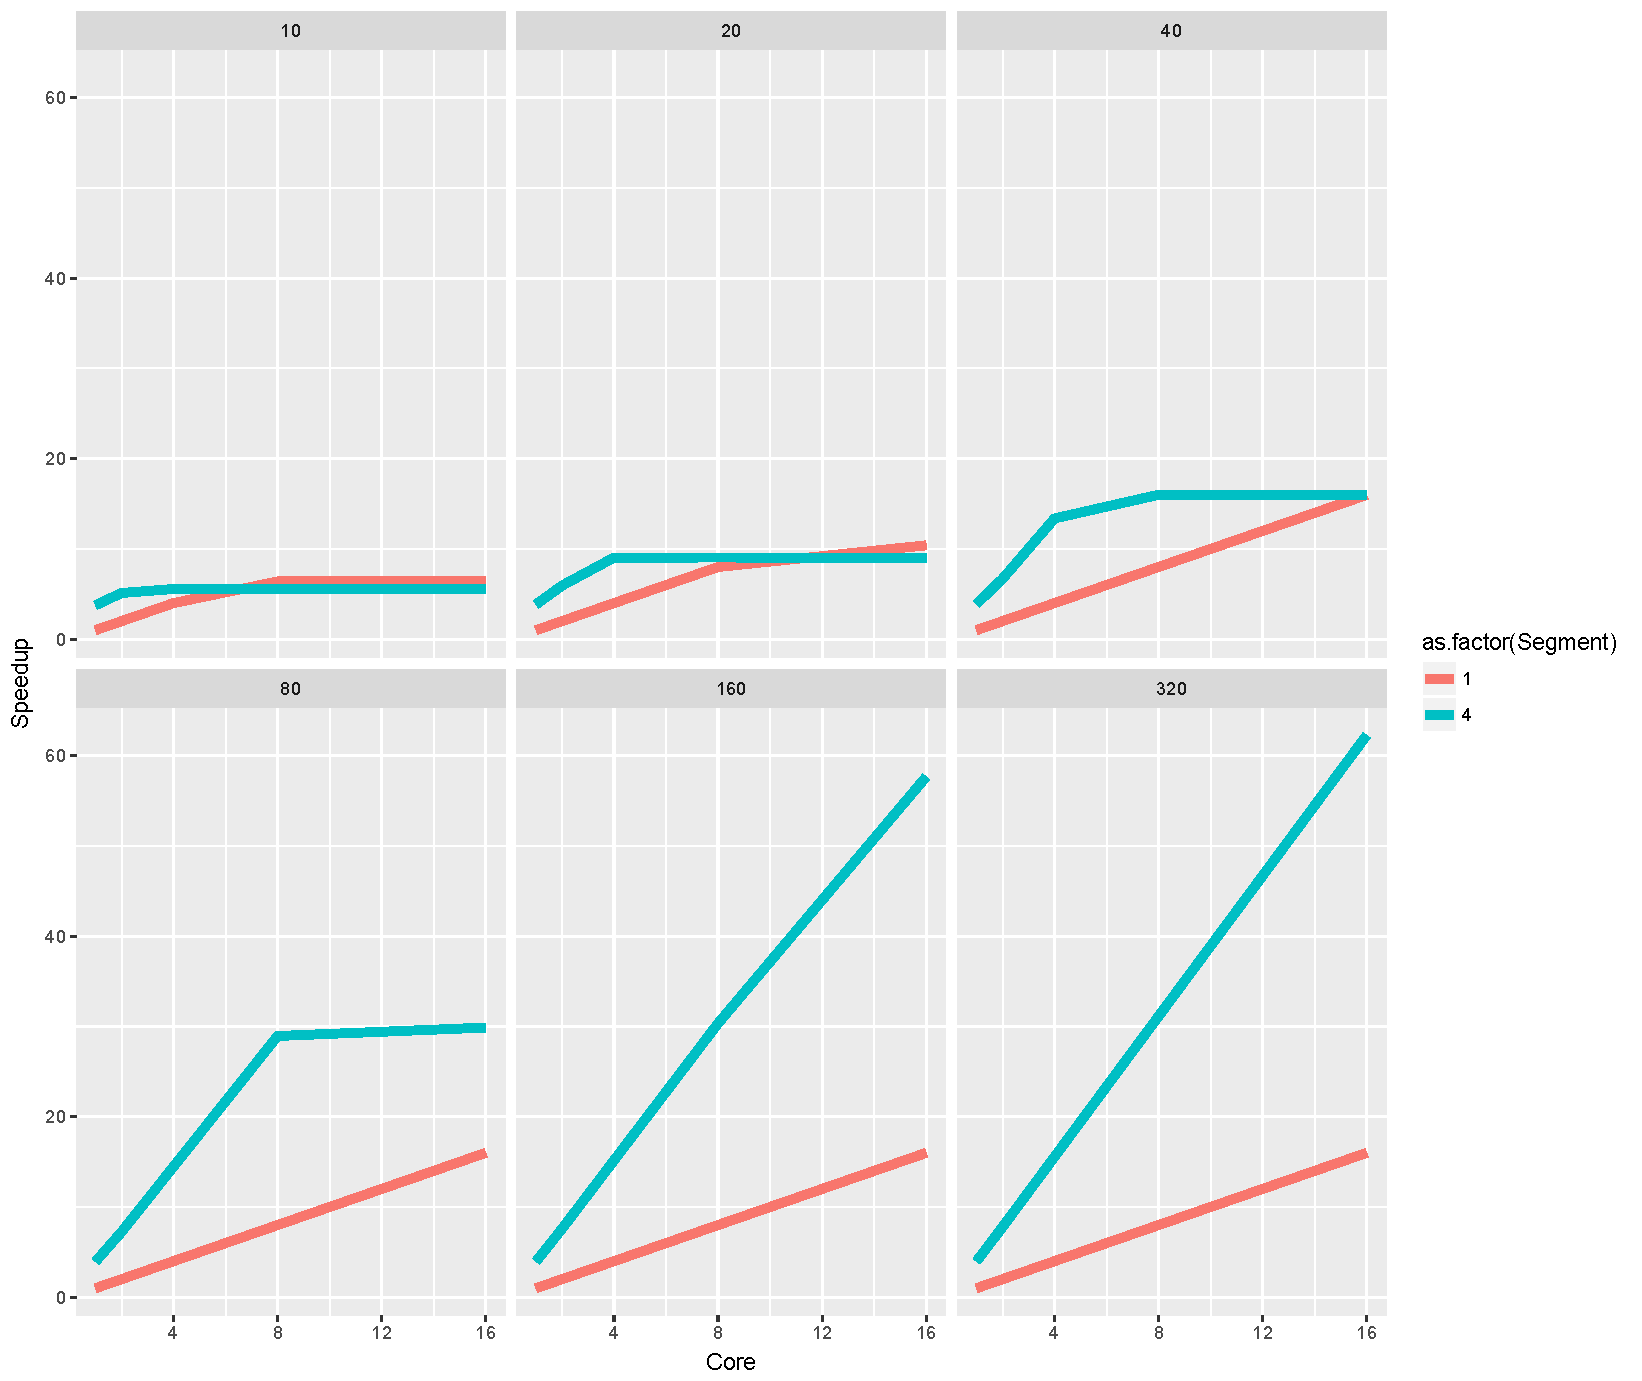
\includegraphics[width=1\textwidth]{chapter3/graphics/total_speed.pdf}
  \caption{Maximum speedup compared to 1 Core 1 Segment}\label{fig:ts}
\end{figure}

\subsection{Comparing segment performanced based on block size (in bytes)}

When blocks are larger than a single icache line, they must be fetched in multime cycles (according to the simulator implementation).
Naturally, we are not always likely to find blocks that fit in a single cache line, even when they are under 25 instructions.
For example we can have floating point instructions with immediates that take up the full 64 bits.
In this section, we look at how changing the size of a 25 or less instructions block will affect performance based on the segments. 
To run experiments, I created blocks of different sizes by injecting floating point operations that use immediates.
This ensures that the blocks can be large whilst staying 25 instructions or less.

Figure~\ref{fig:svl} shows the results of changing the size (in bytes) of a block, given a number of cores fused, the execution time in cycles of a block and the number of segments.
The speedups are obtained in the same fashion as in Figure~\ref{fig:lss}, that is to say I compared 1 Core 1 Segment with 16 Cores 1 Segment or 1 Core 4 Segments with 4 Core 4 Segments (I pair by segment).
In Figure~\ref{fig:svl} the X-Axis facet represents the block size, in this case either 16,40,84,172 or 228 bytes, given that an Icache line in this scenario is 32 bytes.
The Y-axis facet represents the execution time in cycles of a single block, just like in the previous examples.

As we can see from Figure~\ref{fig:svl}, the size of a block does not affect the speedup of single segment cores.
This is to be expected as a fetch request can be sent to another core before the fetch completion of a current block.
Therefore on a single segment, the number of i-cache line requests will not affect the actual performance scaling of adding more cores to a composition.
On the other hand this is clearly not the case for multi-segment cores.
This is simply due to the current limitations of the implementation of the fetching system in the simulator.
Since a core cannot fetch more than a single block at a time for itself, it will have to wait for the current block to finish before fetching the next block.
This does not stop it from sending a fetch request, but it means that it wont act upon that request before the current block is fully fetched.
Because of this, having larger blocks (in bytes) will increase the fetch length drastically.

Now, if the simulator implementation is not the correct implementation (and thus has been incorrect since forever), this would not necessarily fix every problem.
Instead, we would simply end up with the results from Figure~\ref{fig:lss} where we require blocks with long execution time to fully utilise the cores.
This is due to the fact that predictions are still serialised and also happen in a Core-order fashion.
\subsection{Branch Prediction}
In the CASES paper I make the claim that, for a core composition of \textit{X} number of cores, with \text{Y} number of segments must predict $(X*Y)-1$ blocks to ensure every core is fully utilised.
This is due to the fact that there is always a non-speculative block being executed in the chain, so this requires 1 less block to be predicted.
Naturally, this is to ensure full utilisation of every core; in a 4 segmented core, if we are able to correctly predict the first block of the 16th core, then we know that it will at least be used correctly to a certain extent.
Following the equation, I make the claim that we require a certain branch prediction rate to ensure the full utilisation of a core composition.
This equation is simply the number of blocks predicted over the total number of blocks in flight.
For example if we have a 16 core composition with 4 segmented cores, that's 63 divided by 64 so 98\%.
The phrasing I chose in the paper is actually somewhat awkward, as this percentage is a very precise number.
Instead of it being the branch prediction accuracy over the entire application it's actually the branch prediction for a specific \textit{string} of predictions.
Indeed, with a 98\% branch prediction accuracy, if the 1 mispredicted block is the second block in the chain, then the rest of the fetched blocks will still be useless.
So only specifying a percentage is not an accurate representation of what I was trying to convey.
I therefore need to reformulate this percentage of branch prediction accuracy to better describe the problem at hand (and errata it from the previous paper).

\subsection{Conclusion}

Overall we have seen how sensitive 4 segment cores can be; currently they require longer blocks but also require these blocks to not have such a heavy size footprint.
Whilst this may be the case, 4 segments can help alleviate the work from the compiler side as we can fit more blocks onto a single core.
They also provide flexibility, as when blocks grow in terms of instruction size, they become more and more like single-segmented cores.
Since we know that large blocks often require some form of hyper-block formation, which, without profiling information may lead to blocks that contain a lot of wasted space, having the opportunity to fetch more blocks should be much more beneficial.
More segments should also provide more interesting opportunities for scheduling blocks as they allow for more blocks in flight.

\begin{figure}
\center
  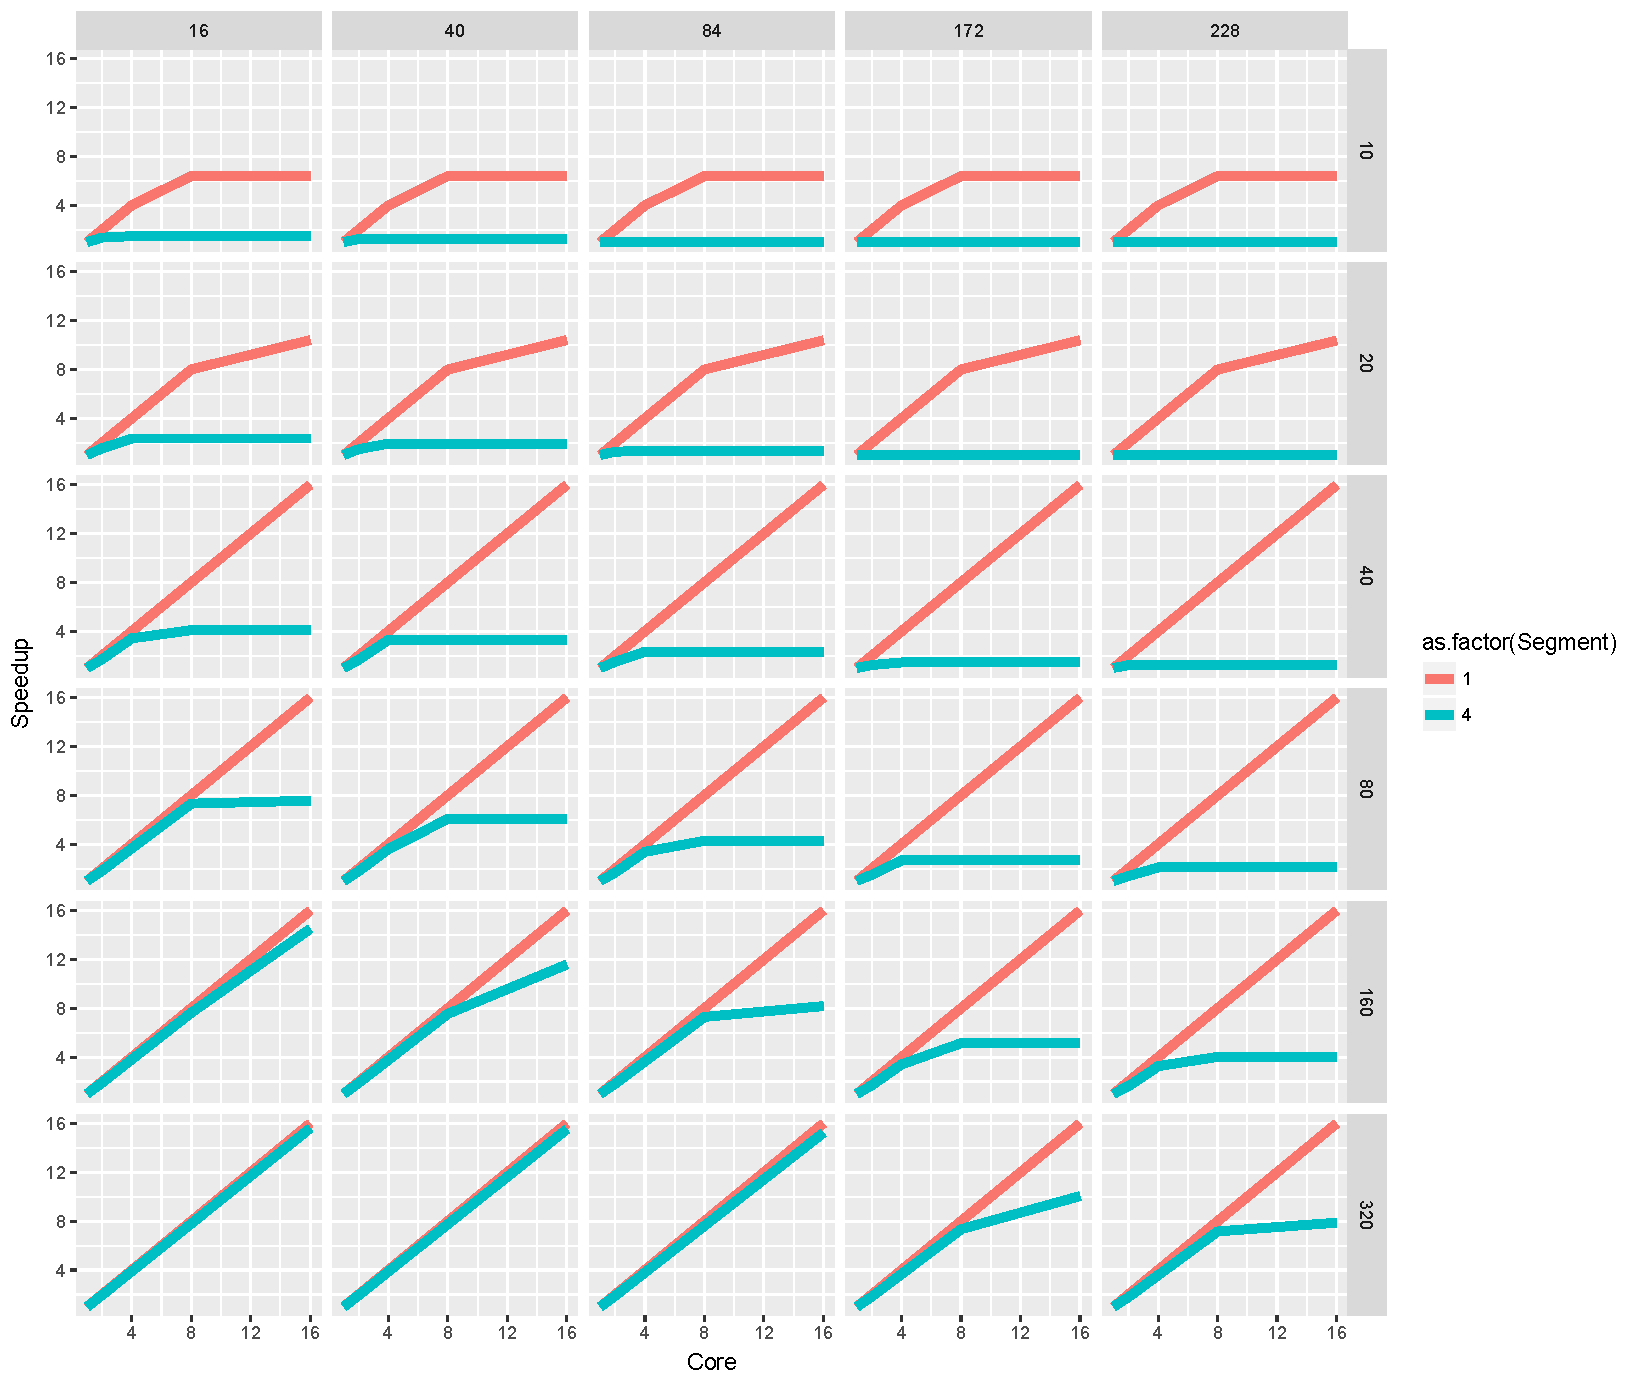
\includegraphics[width=1\textwidth]{chapter3/graphics/size_vs_length.pdf}
  \caption{Speedup by segments.}\label{fig:svl}
\end{figure}

\newpage
\section{What can we do about it?}

\subsection{Unlocking block dispatch}

Currently a core cannot issue a new block if its youngest segment has already submitted a fetch request.
This current restriction means that blocks have to be submitted to cores in a sequential fashion, in other words, if we have 2 cores in a fusion, then C1 cannot fetch a block, send another block to C2 and then fetch a 3rd block. Instead, once it has submitted a block to C2 it will \textbf{have} to wait for C2 to send a new block.
This is what is currently causing cores to wait. Once they have submitted a block to another core, even if their youngest segment commits, they must wait for all other cores in the composition to have fetched blocks so that the fetching wraps back to it.

What I propose as a first step is to try and explore new fetching mechanisms for core-fusion, mainly pipelining fetches.
Instead of "fetching until you're full", a core should start off by making 1 prediction for itself and 1 prediction for the next core in the fusion.
Once it has executed this step it can continue fetching 3 other blocks whilst the next core repeats the process.
This should ensure all cores are fetching 4 blocks almost in parallel.
A paper from 1996 by Andre Seznec et al. from INRIA proposed a multi-block branch predictor that can generate 2 predictions in a single cycle.
We could use this work to do predictions for number of blocks.

Currently, if we have 16 cores, each fetching 4 blocks, if we assume that it takes at least 4 cycles to fetch a block and send a prediction, we have
$fetchlat=(16 * 4)*4$  so 256 cycles before each core has filled up.
By pipelining we can reduce this down to $fetchlat=4+(15*4)+4$  so 68 cycles which is a 3.7x speedup.
Refering back to Figure~\ref{fig:lss}, having an overhed of 68 cycles would place us between the 40 and 80 cycles facet, which means that if we are able to maximize speedup around those facets, that's a 2.6x speedup for a 16 core, 4 segment fusion.
This should, in theory, allow us to better utilise core-fusion as it decreases the restrictions on how long a block should take to execute for a given core-composition size.
Let's recall in the previous report that the overall speedup of a loop, when we only have a single segment can be measured by:
\begin{equation}\label{eq:avspeed}
\frac{Average Execution Time}{\frac{4+4*(Cores -1)+ Average Execution Time + Dependencies  * Cores}{ Cores}}
\end{equation}

In this formula, $4+4*(Cores-1)$ represents the fetch overhead when we have a single segment.
Currently, on 4 segments this would be $4+4*(Cores-1)*4$ which reduces the potential speedup window.

\subsection{Improving branch prediction requirements}

We can use this oportunity of exploring how blocks are fetched to improve overall core-utilisation by ordering the blocks in a different manner.
As we state in the CASES paper, for a core to be useful in a core-fusion, all previous blocks must have been accurately predicted, which can be a huge strain on the branch predictor.
If, instead, we were to send the first prediction made by a core to the following core, we can reduce the stress on the branch predictor.
For example if we had 4 Cores, C1 would have blocks [1,5,9,13] C2:[2,6,10,14], C3:[3,7,11,15] and C4:[4,8,12,16].
In this case, we only need to make 3 predictions to ensure that C4 has at least been somewhat useful.
Previously, in a 16 core composition, if we had 64 blocks in flight, the 16th core could only be considered useful if 60 out of the 64 blocks were considered correct.
This implied at least a 93.7\% accuracy just to ensure that all cores were running some correct code whereas in this new model, only 15 predictions would ensure a utilisation of the core, so dropping it to a mere 23\%.
In Core-Fusion by Ipek et al. Figure 9 shows the distribution of fetch cycles for SPECINT and SPECFP benchmarks.
They define 4 categories: pipeline stalls (cores are busy executing), wrong path (misprediction), FMU stalls (stalls caused by communicating to FMU) and true fetch, which I assume is cycles spent doing actual fetch work.
Whilst they claim that the FMU only causes a 3\% overhead in fetch cycles, they fail to address the fact that, for some benchmarks in SPECINT, mispeculation can caust them up to 50\% of their fetch cycles which is huge.
In these cases they percieve no speedup since they're getting branches wrong almost half the time.
By changing the scheme we can claim that we maintain a higher number of live blocks whilst allowing cores to be useful more frequently.

\subsection{Exploring smarter schedulers}

A lot of the talk in this report is somewhat focused on trying to tackle fetching overhead when we assume blocks are small and take no time to execute.
This most often will only occur in integer heavy blocks, or situations where all data is in cache and blocks are small due to heavy control flow.
However this isn't always the case, and blocks can take a long time to execute.
In these situations, the overhead of fetching isn't the problem but rather which blocks are being fetched and dispatched.
Since we're playing around with how blocks are dispatched we may use this oportunity to look at loops 

\subsection{Introduce a new architecture module}

My plan is to introduce a small module to the architecture which can handle fetch requests made by different cores.
Instead of having a round-robin model, where cores only make fetch requests to other cores once they're full, I intend on having cores submit fetch requests to a module which every core can ping when they are empty.
Using a branch predictor that can make 2 predictions per cycle, we can have each core fetch a block for themselves and send another one to this new module.

The module would simply be a queue that contains a block address and, maybe, the size of the block (in instructions).
The size of the block could be taken from some very small cache, since we don't expect to ever have hundreds of fetch requests being made.
Having the block size in instructions will help avoid situations in which cores pop a request from the module but can't service it due to insufficient segments.
The size should be counted in segments rather than instructions as this reduces the space to a 3 bit field.
I also think we could extend this module to contain a field for scheduling blocks on specific cores.
This way if we, for example, want to schedule blocks in a specific order, we can use this module to filter blocks.
If we can have up to 16 cores in a composition, then that leads to a 4 bit field identifier.
So overall we would only need to cache 7 bits, + some tag to make sure we're pulling the right information (since we can use the address as way to find a cacheline).

\section{How we should evaluate}

\subsection{Simulator}

There are some modifications that have been made and will need to be made to get the results we need.
As of now I have these things implemented:

\begin{itemize}
\item Define custom cycle counts for specific instructions
\item Define a custom branch-prediction accuracy
\item An ITTAGE branch predictor that can be customised to potentially generate 2 predictions per cycle
\item A high-level L2 cache simulation (not very accurate as far as banks or signals go)
\end{itemize}

\subsection{Synthetic Benchmarks}

The first and quickest method of evaluating how block fetching can impact performance is through synthetic benchmarks.
As of now I can think of 3 important parameters for synthetic benchmarks: block size (bytes), block length (cycle), and branch prediction.
By changing these parameters we can determine the most "resilient" method.
Ultimately we want to demonstrate that the current method is ineffective for a large variety of blocks, and also has very little resistance to sequential branch misprediction.

\subsection{Actual benchmarks}

I want to focus on single threaded benchmarks that can help us demonstrate how new block-fetching and block-scheduling algorithms can outperform a more traditional straight forward serial implementation that we have currently.
We essentially want to focus on loops that have a combination of these features:
\begin{itemize}
\item A lot of if-statements (to stress-test branch prediction)
\item Data dependencies
\item Independent iterations
\end{itemize}
I can't think of many more things right now but these can easily come later.